\pdfoutput=1
\def\year{2021}\relax
\documentclass[letterpaper]{article}
\usepackage{aaai21}
\usepackage{times}
\usepackage{helvet}
\usepackage{courier}
\usepackage{url}
\usepackage{graphicx}
\frenchspacing
\setlength{\pdfpagewidth}{8.5in}
\setlength{\pdfpageheight}{11in}
  \pdfinfo{
/Title (A SAT-based Resolution of Lam's Problem: Online Appendix)
}
\usepackage{tikz}
\usepackage{caption}
\newcommand*\elide{\textup{[\,\dots]}}
\nocopyright
\usepackage{amsthm}
\newtheorem{theorem}{Theorem}
\begin{document}
\title{A SAT-based Resolution of Lam's Problem: Online Appendix}
\author{}
\date{}
\maketitle
\addtocounter{table}{1}

\begin{figure}[h!]
\centering
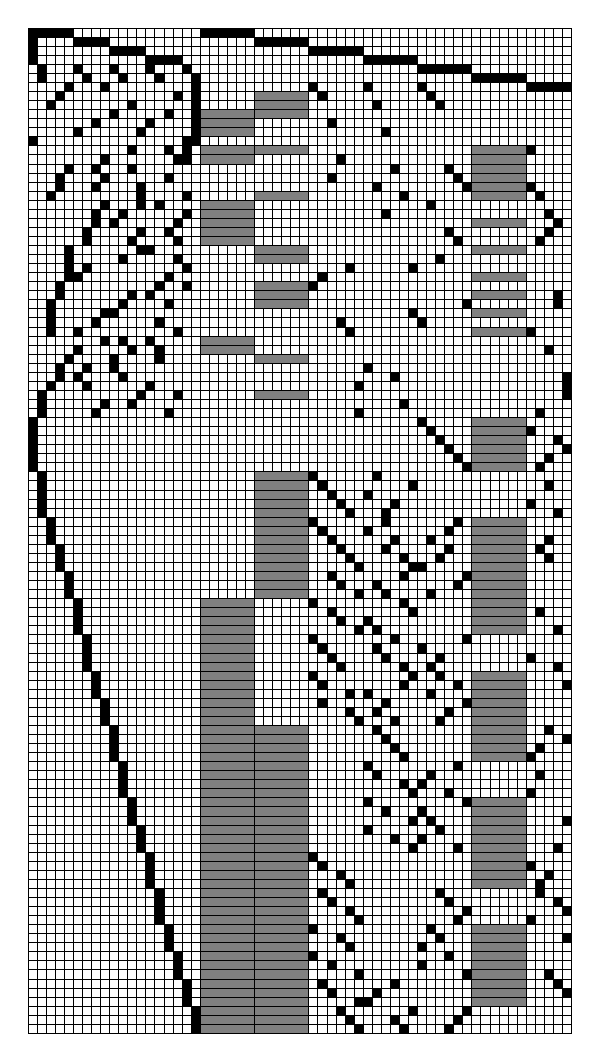
\begin{tikzpicture}[scale=0.115, every node/.style={scale=1}, baseline=(current bounding box.center),ultra thin]
\draw [fill=black] (0,0) rectangle (1,-1);
\draw [fill=black] (1,0) rectangle (2,-1);
\draw [fill=black] (2,0) rectangle (3,-1);
\draw [fill=black] (3,0) rectangle (4,-1);
\draw [fill=black] (4,0) rectangle (5,-1);
\draw (5,0) rectangle (6,-1);
\draw (6,0) rectangle (7,-1);
\draw (7,0) rectangle (8,-1);
\draw (8,0) rectangle (9,-1);
\draw (9,0) rectangle (10,-1);
\draw (10,0) rectangle (11,-1);
\draw (11,0) rectangle (12,-1);
\draw (12,0) rectangle (13,-1);
\draw (13,0) rectangle (14,-1);
\draw (14,0) rectangle (15,-1);
\draw (15,0) rectangle (16,-1);
\draw (16,0) rectangle (17,-1);
\draw (17,0) rectangle (18,-1);
\draw (18,0) rectangle (19,-1);
\draw [fill=black] (19,0) rectangle (20,-1);
\draw [fill=black] (20,0) rectangle (21,-1);
\draw [fill=black] (21,0) rectangle (22,-1);
\draw [fill=black] (22,0) rectangle (23,-1);
\draw [fill=black] (23,0) rectangle (24,-1);
\draw [fill=black] (24,0) rectangle (25,-1);
\draw (25,0) rectangle (26,-1);
\draw (26,0) rectangle (27,-1);
\draw (27,0) rectangle (28,-1);
\draw (28,0) rectangle (29,-1);
\draw (29,0) rectangle (30,-1);
\draw (30,0) rectangle (31,-1);
\draw (31,0) rectangle (32,-1);
\draw (32,0) rectangle (33,-1);
\draw (33,0) rectangle (34,-1);
\draw (34,0) rectangle (35,-1);
\draw (35,0) rectangle (36,-1);
\draw (36,0) rectangle (37,-1);
\draw (37,0) rectangle (38,-1);
\draw (38,0) rectangle (39,-1);
\draw (39,0) rectangle (40,-1);
\draw (40,0) rectangle (41,-1);
\draw (41,0) rectangle (42,-1);
\draw (42,0) rectangle (43,-1);
\draw (43,0) rectangle (44,-1);
\draw (44,0) rectangle (45,-1);
\draw (45,0) rectangle (46,-1);
\draw (46,0) rectangle (47,-1);
\draw (47,0) rectangle (48,-1);
\draw (48,0) rectangle (49,-1);
\draw (49,0) rectangle (50,-1);
\draw (50,0) rectangle (51,-1);
\draw (51,0) rectangle (52,-1);
\draw (52,0) rectangle (53,-1);
\draw (53,0) rectangle (54,-1);
\draw (54,0) rectangle (55,-1);
\draw (55,0) rectangle (56,-1);
\draw (56,0) rectangle (57,-1);
\draw (57,0) rectangle (58,-1);
\draw (58,0) rectangle (59,-1);
\draw (59,0) rectangle (60,-1);
\draw [fill=black] (0,-1) rectangle (1,-2);
\draw (1,-1) rectangle (2,-2);
\draw (2,-1) rectangle (3,-2);
\draw (3,-1) rectangle (4,-2);
\draw (4,-1) rectangle (5,-2);
\draw [fill=black] (5,-1) rectangle (6,-2);
\draw [fill=black] (6,-1) rectangle (7,-2);
\draw [fill=black] (7,-1) rectangle (8,-2);
\draw [fill=black] (8,-1) rectangle (9,-2);
\draw (9,-1) rectangle (10,-2);
\draw (10,-1) rectangle (11,-2);
\draw (11,-1) rectangle (12,-2);
\draw (12,-1) rectangle (13,-2);
\draw (13,-1) rectangle (14,-2);
\draw (14,-1) rectangle (15,-2);
\draw (15,-1) rectangle (16,-2);
\draw (16,-1) rectangle (17,-2);
\draw (17,-1) rectangle (18,-2);
\draw (18,-1) rectangle (19,-2);
\draw (19,-1) rectangle (20,-2);
\draw (20,-1) rectangle (21,-2);
\draw (21,-1) rectangle (22,-2);
\draw (22,-1) rectangle (23,-2);
\draw (23,-1) rectangle (24,-2);
\draw (24,-1) rectangle (25,-2);
\draw [fill=black] (25,-1) rectangle (26,-2);
\draw [fill=black] (26,-1) rectangle (27,-2);
\draw [fill=black] (27,-1) rectangle (28,-2);
\draw [fill=black] (28,-1) rectangle (29,-2);
\draw [fill=black] (29,-1) rectangle (30,-2);
\draw [fill=black] (30,-1) rectangle (31,-2);
\draw (31,-1) rectangle (32,-2);
\draw (32,-1) rectangle (33,-2);
\draw (33,-1) rectangle (34,-2);
\draw (34,-1) rectangle (35,-2);
\draw (35,-1) rectangle (36,-2);
\draw (36,-1) rectangle (37,-2);
\draw (37,-1) rectangle (38,-2);
\draw (38,-1) rectangle (39,-2);
\draw (39,-1) rectangle (40,-2);
\draw (40,-1) rectangle (41,-2);
\draw (41,-1) rectangle (42,-2);
\draw (42,-1) rectangle (43,-2);
\draw (43,-1) rectangle (44,-2);
\draw (44,-1) rectangle (45,-2);
\draw (45,-1) rectangle (46,-2);
\draw (46,-1) rectangle (47,-2);
\draw (47,-1) rectangle (48,-2);
\draw (48,-1) rectangle (49,-2);
\draw (49,-1) rectangle (50,-2);
\draw (50,-1) rectangle (51,-2);
\draw (51,-1) rectangle (52,-2);
\draw (52,-1) rectangle (53,-2);
\draw (53,-1) rectangle (54,-2);
\draw (54,-1) rectangle (55,-2);
\draw (55,-1) rectangle (56,-2);
\draw (56,-1) rectangle (57,-2);
\draw (57,-1) rectangle (58,-2);
\draw (58,-1) rectangle (59,-2);
\draw (59,-1) rectangle (60,-2);
\draw [fill=black] (0,-2) rectangle (1,-3);
\draw (1,-2) rectangle (2,-3);
\draw (2,-2) rectangle (3,-3);
\draw (3,-2) rectangle (4,-3);
\draw (4,-2) rectangle (5,-3);
\draw (5,-2) rectangle (6,-3);
\draw (6,-2) rectangle (7,-3);
\draw (7,-2) rectangle (8,-3);
\draw (8,-2) rectangle (9,-3);
\draw [fill=black] (9,-2) rectangle (10,-3);
\draw [fill=black] (10,-2) rectangle (11,-3);
\draw [fill=black] (11,-2) rectangle (12,-3);
\draw [fill=black] (12,-2) rectangle (13,-3);
\draw (13,-2) rectangle (14,-3);
\draw (14,-2) rectangle (15,-3);
\draw (15,-2) rectangle (16,-3);
\draw (16,-2) rectangle (17,-3);
\draw (17,-2) rectangle (18,-3);
\draw (18,-2) rectangle (19,-3);
\draw (19,-2) rectangle (20,-3);
\draw (20,-2) rectangle (21,-3);
\draw (21,-2) rectangle (22,-3);
\draw (22,-2) rectangle (23,-3);
\draw (23,-2) rectangle (24,-3);
\draw (24,-2) rectangle (25,-3);
\draw (25,-2) rectangle (26,-3);
\draw (26,-2) rectangle (27,-3);
\draw (27,-2) rectangle (28,-3);
\draw (28,-2) rectangle (29,-3);
\draw (29,-2) rectangle (30,-3);
\draw (30,-2) rectangle (31,-3);
\draw [fill=black] (31,-2) rectangle (32,-3);
\draw [fill=black] (32,-2) rectangle (33,-3);
\draw [fill=black] (33,-2) rectangle (34,-3);
\draw [fill=black] (34,-2) rectangle (35,-3);
\draw [fill=black] (35,-2) rectangle (36,-3);
\draw [fill=black] (36,-2) rectangle (37,-3);
\draw (37,-2) rectangle (38,-3);
\draw (38,-2) rectangle (39,-3);
\draw (39,-2) rectangle (40,-3);
\draw (40,-2) rectangle (41,-3);
\draw (41,-2) rectangle (42,-3);
\draw (42,-2) rectangle (43,-3);
\draw (43,-2) rectangle (44,-3);
\draw (44,-2) rectangle (45,-3);
\draw (45,-2) rectangle (46,-3);
\draw (46,-2) rectangle (47,-3);
\draw (47,-2) rectangle (48,-3);
\draw (48,-2) rectangle (49,-3);
\draw (49,-2) rectangle (50,-3);
\draw (50,-2) rectangle (51,-3);
\draw (51,-2) rectangle (52,-3);
\draw (52,-2) rectangle (53,-3);
\draw (53,-2) rectangle (54,-3);
\draw (54,-2) rectangle (55,-3);
\draw (55,-2) rectangle (56,-3);
\draw (56,-2) rectangle (57,-3);
\draw (57,-2) rectangle (58,-3);
\draw (58,-2) rectangle (59,-3);
\draw (59,-2) rectangle (60,-3);
\draw [fill=black] (0,-3) rectangle (1,-4);
\draw (1,-3) rectangle (2,-4);
\draw (2,-3) rectangle (3,-4);
\draw (3,-3) rectangle (4,-4);
\draw (4,-3) rectangle (5,-4);
\draw (5,-3) rectangle (6,-4);
\draw (6,-3) rectangle (7,-4);
\draw (7,-3) rectangle (8,-4);
\draw (8,-3) rectangle (9,-4);
\draw (9,-3) rectangle (10,-4);
\draw (10,-3) rectangle (11,-4);
\draw (11,-3) rectangle (12,-4);
\draw (12,-3) rectangle (13,-4);
\draw [fill=black] (13,-3) rectangle (14,-4);
\draw [fill=black] (14,-3) rectangle (15,-4);
\draw [fill=black] (15,-3) rectangle (16,-4);
\draw [fill=black] (16,-3) rectangle (17,-4);
\draw (17,-3) rectangle (18,-4);
\draw (18,-3) rectangle (19,-4);
\draw (19,-3) rectangle (20,-4);
\draw (20,-3) rectangle (21,-4);
\draw (21,-3) rectangle (22,-4);
\draw (22,-3) rectangle (23,-4);
\draw (23,-3) rectangle (24,-4);
\draw (24,-3) rectangle (25,-4);
\draw (25,-3) rectangle (26,-4);
\draw (26,-3) rectangle (27,-4);
\draw (27,-3) rectangle (28,-4);
\draw (28,-3) rectangle (29,-4);
\draw (29,-3) rectangle (30,-4);
\draw (30,-3) rectangle (31,-4);
\draw (31,-3) rectangle (32,-4);
\draw (32,-3) rectangle (33,-4);
\draw (33,-3) rectangle (34,-4);
\draw (34,-3) rectangle (35,-4);
\draw (35,-3) rectangle (36,-4);
\draw (36,-3) rectangle (37,-4);
\draw [fill=black] (37,-3) rectangle (38,-4);
\draw [fill=black] (38,-3) rectangle (39,-4);
\draw [fill=black] (39,-3) rectangle (40,-4);
\draw [fill=black] (40,-3) rectangle (41,-4);
\draw [fill=black] (41,-3) rectangle (42,-4);
\draw [fill=black] (42,-3) rectangle (43,-4);
\draw (43,-3) rectangle (44,-4);
\draw (44,-3) rectangle (45,-4);
\draw (45,-3) rectangle (46,-4);
\draw (46,-3) rectangle (47,-4);
\draw (47,-3) rectangle (48,-4);
\draw (48,-3) rectangle (49,-4);
\draw (49,-3) rectangle (50,-4);
\draw (50,-3) rectangle (51,-4);
\draw (51,-3) rectangle (52,-4);
\draw (52,-3) rectangle (53,-4);
\draw (53,-3) rectangle (54,-4);
\draw (54,-3) rectangle (55,-4);
\draw (55,-3) rectangle (56,-4);
\draw (56,-3) rectangle (57,-4);
\draw (57,-3) rectangle (58,-4);
\draw (58,-3) rectangle (59,-4);
\draw (59,-3) rectangle (60,-4);
\draw (0,-4) rectangle (1,-5);
\draw [fill=black] (1,-4) rectangle (2,-5);
\draw (2,-4) rectangle (3,-5);
\draw (3,-4) rectangle (4,-5);
\draw (4,-4) rectangle (5,-5);
\draw [fill=black] (5,-4) rectangle (6,-5);
\draw (6,-4) rectangle (7,-5);
\draw (7,-4) rectangle (8,-5);
\draw (8,-4) rectangle (9,-5);
\draw [fill=black] (9,-4) rectangle (10,-5);
\draw (10,-4) rectangle (11,-5);
\draw (11,-4) rectangle (12,-5);
\draw (12,-4) rectangle (13,-5);
\draw [fill=black] (13,-4) rectangle (14,-5);
\draw (14,-4) rectangle (15,-5);
\draw (15,-4) rectangle (16,-5);
\draw (16,-4) rectangle (17,-5);
\draw [fill=black] (17,-4) rectangle (18,-5);
\draw (18,-4) rectangle (19,-5);
\draw (19,-4) rectangle (20,-5);
\draw (20,-4) rectangle (21,-5);
\draw (21,-4) rectangle (22,-5);
\draw (22,-4) rectangle (23,-5);
\draw (23,-4) rectangle (24,-5);
\draw (24,-4) rectangle (25,-5);
\draw (25,-4) rectangle (26,-5);
\draw (26,-4) rectangle (27,-5);
\draw (27,-4) rectangle (28,-5);
\draw (28,-4) rectangle (29,-5);
\draw (29,-4) rectangle (30,-5);
\draw (30,-4) rectangle (31,-5);
\draw (31,-4) rectangle (32,-5);
\draw (32,-4) rectangle (33,-5);
\draw (33,-4) rectangle (34,-5);
\draw (34,-4) rectangle (35,-5);
\draw (35,-4) rectangle (36,-5);
\draw (36,-4) rectangle (37,-5);
\draw (37,-4) rectangle (38,-5);
\draw (38,-4) rectangle (39,-5);
\draw (39,-4) rectangle (40,-5);
\draw (40,-4) rectangle (41,-5);
\draw (41,-4) rectangle (42,-5);
\draw (42,-4) rectangle (43,-5);
\draw [fill=black] (43,-4) rectangle (44,-5);
\draw [fill=black] (44,-4) rectangle (45,-5);
\draw [fill=black] (45,-4) rectangle (46,-5);
\draw [fill=black] (46,-4) rectangle (47,-5);
\draw [fill=black] (47,-4) rectangle (48,-5);
\draw [fill=black] (48,-4) rectangle (49,-5);
\draw (49,-4) rectangle (50,-5);
\draw (50,-4) rectangle (51,-5);
\draw (51,-4) rectangle (52,-5);
\draw (52,-4) rectangle (53,-5);
\draw (53,-4) rectangle (54,-5);
\draw (54,-4) rectangle (55,-5);
\draw (55,-4) rectangle (56,-5);
\draw (56,-4) rectangle (57,-5);
\draw (57,-4) rectangle (58,-5);
\draw (58,-4) rectangle (59,-5);
\draw (59,-4) rectangle (60,-5);
\draw (0,-5) rectangle (1,-6);
\draw [fill=black] (1,-5) rectangle (2,-6);
\draw (2,-5) rectangle (3,-6);
\draw (3,-5) rectangle (4,-6);
\draw (4,-5) rectangle (5,-6);
\draw (5,-5) rectangle (6,-6);
\draw [fill=black] (6,-5) rectangle (7,-6);
\draw (7,-5) rectangle (8,-6);
\draw (8,-5) rectangle (9,-6);
\draw (9,-5) rectangle (10,-6);
\draw [fill=black] (10,-5) rectangle (11,-6);
\draw (11,-5) rectangle (12,-6);
\draw (12,-5) rectangle (13,-6);
\draw (13,-5) rectangle (14,-6);
\draw [fill=black] (14,-5) rectangle (15,-6);
\draw (15,-5) rectangle (16,-6);
\draw (16,-5) rectangle (17,-6);
\draw (17,-5) rectangle (18,-6);
\draw [fill=black] (18,-5) rectangle (19,-6);
\draw (19,-5) rectangle (20,-6);
\draw (20,-5) rectangle (21,-6);
\draw (21,-5) rectangle (22,-6);
\draw (22,-5) rectangle (23,-6);
\draw (23,-5) rectangle (24,-6);
\draw (24,-5) rectangle (25,-6);
\draw (25,-5) rectangle (26,-6);
\draw (26,-5) rectangle (27,-6);
\draw (27,-5) rectangle (28,-6);
\draw (28,-5) rectangle (29,-6);
\draw (29,-5) rectangle (30,-6);
\draw (30,-5) rectangle (31,-6);
\draw (31,-5) rectangle (32,-6);
\draw (32,-5) rectangle (33,-6);
\draw (33,-5) rectangle (34,-6);
\draw (34,-5) rectangle (35,-6);
\draw (35,-5) rectangle (36,-6);
\draw (36,-5) rectangle (37,-6);
\draw (37,-5) rectangle (38,-6);
\draw (38,-5) rectangle (39,-6);
\draw (39,-5) rectangle (40,-6);
\draw (40,-5) rectangle (41,-6);
\draw (41,-5) rectangle (42,-6);
\draw (42,-5) rectangle (43,-6);
\draw (43,-5) rectangle (44,-6);
\draw (44,-5) rectangle (45,-6);
\draw (45,-5) rectangle (46,-6);
\draw (46,-5) rectangle (47,-6);
\draw (47,-5) rectangle (48,-6);
\draw (48,-5) rectangle (49,-6);
\draw [fill=black] (49,-5) rectangle (50,-6);
\draw [fill=black] (50,-5) rectangle (51,-6);
\draw [fill=black] (51,-5) rectangle (52,-6);
\draw [fill=black] (52,-5) rectangle (53,-6);
\draw [fill=black] (53,-5) rectangle (54,-6);
\draw [fill=black] (54,-5) rectangle (55,-6);
\draw (55,-5) rectangle (56,-6);
\draw (56,-5) rectangle (57,-6);
\draw (57,-5) rectangle (58,-6);
\draw (58,-5) rectangle (59,-6);
\draw (59,-5) rectangle (60,-6);
\draw (0,-6) rectangle (1,-7);
\draw (1,-6) rectangle (2,-7);
\draw (2,-6) rectangle (3,-7);
\draw (3,-6) rectangle (4,-7);
\draw [fill=black] (4,-6) rectangle (5,-7);
\draw (5,-6) rectangle (6,-7);
\draw (6,-6) rectangle (7,-7);
\draw (7,-6) rectangle (8,-7);
\draw [fill=black] (8,-6) rectangle (9,-7);
\draw (9,-6) rectangle (10,-7);
\draw (10,-6) rectangle (11,-7);
\draw (11,-6) rectangle (12,-7);
\draw (12,-6) rectangle (13,-7);
\draw (13,-6) rectangle (14,-7);
\draw (14,-6) rectangle (15,-7);
\draw (15,-6) rectangle (16,-7);
\draw (16,-6) rectangle (17,-7);
\draw (17,-6) rectangle (18,-7);
\draw [fill=black] (18,-6) rectangle (19,-7);
\draw (19,-6) rectangle (20,-7);
\draw (20,-6) rectangle (21,-7);
\draw (21,-6) rectangle (22,-7);
\draw (22,-6) rectangle (23,-7);
\draw (23,-6) rectangle (24,-7);
\draw (24,-6) rectangle (25,-7);
\draw (25,-6) rectangle (26,-7);
\draw (26,-6) rectangle (27,-7);
\draw (27,-6) rectangle (28,-7);
\draw (28,-6) rectangle (29,-7);
\draw (29,-6) rectangle (30,-7);
\draw (30,-6) rectangle (31,-7);
\draw [fill=black] (31,-6) rectangle (32,-7);
\draw (32,-6) rectangle (33,-7);
\draw (33,-6) rectangle (34,-7);
\draw (34,-6) rectangle (35,-7);
\draw (35,-6) rectangle (36,-7);
\draw (36,-6) rectangle (37,-7);
\draw [fill=black] (37,-6) rectangle (38,-7);
\draw (38,-6) rectangle (39,-7);
\draw (39,-6) rectangle (40,-7);
\draw (40,-6) rectangle (41,-7);
\draw (41,-6) rectangle (42,-7);
\draw (42,-6) rectangle (43,-7);
\draw [fill=black] (43,-6) rectangle (44,-7);
\draw (44,-6) rectangle (45,-7);
\draw (45,-6) rectangle (46,-7);
\draw (46,-6) rectangle (47,-7);
\draw (47,-6) rectangle (48,-7);
\draw (48,-6) rectangle (49,-7);
\draw (49,-6) rectangle (50,-7);
\draw (50,-6) rectangle (51,-7);
\draw (51,-6) rectangle (52,-7);
\draw (52,-6) rectangle (53,-7);
\draw (53,-6) rectangle (54,-7);
\draw (54,-6) rectangle (55,-7);
\draw [fill=black] (55,-6) rectangle (56,-7);
\draw [fill=black] (56,-6) rectangle (57,-7);
\draw [fill=black] (57,-6) rectangle (58,-7);
\draw [fill=black] (58,-6) rectangle (59,-7);
\draw [fill=black] (59,-6) rectangle (60,-7);
\draw (0,-7) rectangle (1,-8);
\draw (1,-7) rectangle (2,-8);
\draw (2,-7) rectangle (3,-8);
\draw [fill=black] (3,-7) rectangle (4,-8);
\draw (4,-7) rectangle (5,-8);
\draw (5,-7) rectangle (6,-8);
\draw (6,-7) rectangle (7,-8);
\draw (7,-7) rectangle (8,-8);
\draw (8,-7) rectangle (9,-8);
\draw (9,-7) rectangle (10,-8);
\draw (10,-7) rectangle (11,-8);
\draw (11,-7) rectangle (12,-8);
\draw (12,-7) rectangle (13,-8);
\draw (13,-7) rectangle (14,-8);
\draw (14,-7) rectangle (15,-8);
\draw (15,-7) rectangle (16,-8);
\draw [fill=black] (16,-7) rectangle (17,-8);
\draw (17,-7) rectangle (18,-8);
\draw [fill=black] (18,-7) rectangle (19,-8);
\draw (19,-7) rectangle (20,-8);
\draw (20,-7) rectangle (21,-8);
\draw (21,-7) rectangle (22,-8);
\draw (22,-7) rectangle (23,-8);
\draw (23,-7) rectangle (24,-8);
\draw (24,-7) rectangle (25,-8);
\draw [fill=gray] (25,-7) rectangle (31,-8);
\draw (31,-7) rectangle (32,-8);
\draw [fill=black] (32,-7) rectangle (33,-8);
\draw (33,-7) rectangle (34,-8);
\draw (34,-7) rectangle (35,-8);
\draw (35,-7) rectangle (36,-8);
\draw (36,-7) rectangle (37,-8);
\draw (37,-7) rectangle (38,-8);
\draw (38,-7) rectangle (39,-8);
\draw (39,-7) rectangle (40,-8);
\draw (40,-7) rectangle (41,-8);
\draw (41,-7) rectangle (42,-8);
\draw (42,-7) rectangle (43,-8);
\draw (43,-7) rectangle (44,-8);
\draw [fill=black] (44,-7) rectangle (45,-8);
\draw (45,-7) rectangle (46,-8);
\draw (46,-7) rectangle (47,-8);
\draw (47,-7) rectangle (48,-8);
\draw (48,-7) rectangle (49,-8);
\draw (49,-7) rectangle (50,-8);
\draw (50,-7) rectangle (51,-8);
\draw (51,-7) rectangle (52,-8);
\draw (52,-7) rectangle (53,-8);
\draw (53,-7) rectangle (54,-8);
\draw (54,-7) rectangle (55,-8);
\draw (55,-7) rectangle (56,-8);
\draw (56,-7) rectangle (57,-8);
\draw (57,-7) rectangle (58,-8);
\draw (58,-7) rectangle (59,-8);
\draw (59,-7) rectangle (60,-8);
\draw (0,-8) rectangle (1,-9);
\draw (1,-8) rectangle (2,-9);
\draw [fill=black] (2,-8) rectangle (3,-9);
\draw (3,-8) rectangle (4,-9);
\draw (4,-8) rectangle (5,-9);
\draw (5,-8) rectangle (6,-9);
\draw (6,-8) rectangle (7,-9);
\draw (7,-8) rectangle (8,-9);
\draw (8,-8) rectangle (9,-9);
\draw (9,-8) rectangle (10,-9);
\draw (10,-8) rectangle (11,-9);
\draw [fill=black] (11,-8) rectangle (12,-9);
\draw (12,-8) rectangle (13,-9);
\draw (13,-8) rectangle (14,-9);
\draw (14,-8) rectangle (15,-9);
\draw (15,-8) rectangle (16,-9);
\draw (16,-8) rectangle (17,-9);
\draw (17,-8) rectangle (18,-9);
\draw [fill=black] (18,-8) rectangle (19,-9);
\draw (19,-8) rectangle (20,-9);
\draw (20,-8) rectangle (21,-9);
\draw (21,-8) rectangle (22,-9);
\draw (22,-8) rectangle (23,-9);
\draw (23,-8) rectangle (24,-9);
\draw (24,-8) rectangle (25,-9);
\draw [fill=gray] (25,-8) rectangle (31,-9);
\draw (31,-8) rectangle (32,-9);
\draw (32,-8) rectangle (33,-9);
\draw (33,-8) rectangle (34,-9);
\draw (34,-8) rectangle (35,-9);
\draw (35,-8) rectangle (36,-9);
\draw (36,-8) rectangle (37,-9);
\draw (37,-8) rectangle (38,-9);
\draw [fill=black] (38,-8) rectangle (39,-9);
\draw (39,-8) rectangle (40,-9);
\draw (40,-8) rectangle (41,-9);
\draw (41,-8) rectangle (42,-9);
\draw (42,-8) rectangle (43,-9);
\draw (43,-8) rectangle (44,-9);
\draw (44,-8) rectangle (45,-9);
\draw [fill=black] (45,-8) rectangle (46,-9);
\draw (46,-8) rectangle (47,-9);
\draw (47,-8) rectangle (48,-9);
\draw (48,-8) rectangle (49,-9);
\draw (49,-8) rectangle (50,-9);
\draw (50,-8) rectangle (51,-9);
\draw (51,-8) rectangle (52,-9);
\draw (52,-8) rectangle (53,-9);
\draw (53,-8) rectangle (54,-9);
\draw (54,-8) rectangle (55,-9);
\draw (55,-8) rectangle (56,-9);
\draw (56,-8) rectangle (57,-9);
\draw (57,-8) rectangle (58,-9);
\draw (58,-8) rectangle (59,-9);
\draw (59,-8) rectangle (60,-9);
\draw (0,-9) rectangle (1,-10);
\draw (1,-9) rectangle (2,-10);
\draw (2,-9) rectangle (3,-10);
\draw (3,-9) rectangle (4,-10);
\draw (4,-9) rectangle (5,-10);
\draw (5,-9) rectangle (6,-10);
\draw (6,-9) rectangle (7,-10);
\draw (7,-9) rectangle (8,-10);
\draw (8,-9) rectangle (9,-10);
\draw [fill=black] (9,-9) rectangle (10,-10);
\draw (10,-9) rectangle (11,-10);
\draw (11,-9) rectangle (12,-10);
\draw (12,-9) rectangle (13,-10);
\draw (13,-9) rectangle (14,-10);
\draw (14,-9) rectangle (15,-10);
\draw [fill=black] (15,-9) rectangle (16,-10);
\draw (16,-9) rectangle (17,-10);
\draw (17,-9) rectangle (18,-10);
\draw [fill=black] (18,-9) rectangle (19,-10);
\draw [fill=gray] (19,-9) rectangle (25,-10);
\draw [fill=gray] (25,-9) rectangle (31,-10);
\draw (31,-9) rectangle (32,-10);
\draw (32,-9) rectangle (33,-10);
\draw (33,-9) rectangle (34,-10);
\draw (34,-9) rectangle (35,-10);
\draw (35,-9) rectangle (36,-10);
\draw (36,-9) rectangle (37,-10);
\draw (37,-9) rectangle (38,-10);
\draw (38,-9) rectangle (39,-10);
\draw (39,-9) rectangle (40,-10);
\draw (40,-9) rectangle (41,-10);
\draw (41,-9) rectangle (42,-10);
\draw (42,-9) rectangle (43,-10);
\draw (43,-9) rectangle (44,-10);
\draw (44,-9) rectangle (45,-10);
\draw (45,-9) rectangle (46,-10);
\draw (46,-9) rectangle (47,-10);
\draw (47,-9) rectangle (48,-10);
\draw (48,-9) rectangle (49,-10);
\draw (49,-9) rectangle (50,-10);
\draw (50,-9) rectangle (51,-10);
\draw (51,-9) rectangle (52,-10);
\draw (52,-9) rectangle (53,-10);
\draw (53,-9) rectangle (54,-10);
\draw (54,-9) rectangle (55,-10);
\draw (55,-9) rectangle (56,-10);
\draw (56,-9) rectangle (57,-10);
\draw (57,-9) rectangle (58,-10);
\draw (58,-9) rectangle (59,-10);
\draw (59,-9) rectangle (60,-10);
\draw (0,-10) rectangle (1,-11);
\draw (1,-10) rectangle (2,-11);
\draw (2,-10) rectangle (3,-11);
\draw (3,-10) rectangle (4,-11);
\draw (4,-10) rectangle (5,-11);
\draw (5,-10) rectangle (6,-11);
\draw (6,-10) rectangle (7,-11);
\draw [fill=black] (7,-10) rectangle (8,-11);
\draw (8,-10) rectangle (9,-11);
\draw (9,-10) rectangle (10,-11);
\draw (10,-10) rectangle (11,-11);
\draw (11,-10) rectangle (12,-11);
\draw (12,-10) rectangle (13,-11);
\draw [fill=black] (13,-10) rectangle (14,-11);
\draw (14,-10) rectangle (15,-11);
\draw (15,-10) rectangle (16,-11);
\draw (16,-10) rectangle (17,-11);
\draw (17,-10) rectangle (18,-11);
\draw [fill=black] (18,-10) rectangle (19,-11);
\draw [fill=gray] (19,-10) rectangle (25,-11);
\draw (25,-10) rectangle (26,-11);
\draw (26,-10) rectangle (27,-11);
\draw (27,-10) rectangle (28,-11);
\draw (28,-10) rectangle (29,-11);
\draw (29,-10) rectangle (30,-11);
\draw (30,-10) rectangle (31,-11);
\draw (31,-10) rectangle (32,-11);
\draw (32,-10) rectangle (33,-11);
\draw [fill=black] (33,-10) rectangle (34,-11);
\draw (34,-10) rectangle (35,-11);
\draw (35,-10) rectangle (36,-11);
\draw (36,-10) rectangle (37,-11);
\draw (37,-10) rectangle (38,-11);
\draw (38,-10) rectangle (39,-11);
\draw (39,-10) rectangle (40,-11);
\draw (40,-10) rectangle (41,-11);
\draw (41,-10) rectangle (42,-11);
\draw (42,-10) rectangle (43,-11);
\draw (43,-10) rectangle (44,-11);
\draw (44,-10) rectangle (45,-11);
\draw (45,-10) rectangle (46,-11);
\draw (46,-10) rectangle (47,-11);
\draw (47,-10) rectangle (48,-11);
\draw (48,-10) rectangle (49,-11);
\draw (49,-10) rectangle (50,-11);
\draw (50,-10) rectangle (51,-11);
\draw (51,-10) rectangle (52,-11);
\draw (52,-10) rectangle (53,-11);
\draw (53,-10) rectangle (54,-11);
\draw (54,-10) rectangle (55,-11);
\draw (55,-10) rectangle (56,-11);
\draw (56,-10) rectangle (57,-11);
\draw (57,-10) rectangle (58,-11);
\draw (58,-10) rectangle (59,-11);
\draw (59,-10) rectangle (60,-11);
\draw (0,-11) rectangle (1,-12);
\draw (1,-11) rectangle (2,-12);
\draw (2,-11) rectangle (3,-12);
\draw (3,-11) rectangle (4,-12);
\draw (4,-11) rectangle (5,-12);
\draw [fill=black] (5,-11) rectangle (6,-12);
\draw (6,-11) rectangle (7,-12);
\draw (7,-11) rectangle (8,-12);
\draw (8,-11) rectangle (9,-12);
\draw (9,-11) rectangle (10,-12);
\draw (10,-11) rectangle (11,-12);
\draw (11,-11) rectangle (12,-12);
\draw [fill=black] (12,-11) rectangle (13,-12);
\draw (13,-11) rectangle (14,-12);
\draw (14,-11) rectangle (15,-12);
\draw (15,-11) rectangle (16,-12);
\draw (16,-11) rectangle (17,-12);
\draw (17,-11) rectangle (18,-12);
\draw [fill=black] (18,-11) rectangle (19,-12);
\draw [fill=gray] (19,-11) rectangle (25,-12);
\draw (25,-11) rectangle (26,-12);
\draw (26,-11) rectangle (27,-12);
\draw (27,-11) rectangle (28,-12);
\draw (28,-11) rectangle (29,-12);
\draw (29,-11) rectangle (30,-12);
\draw (30,-11) rectangle (31,-12);
\draw (31,-11) rectangle (32,-12);
\draw (32,-11) rectangle (33,-12);
\draw (33,-11) rectangle (34,-12);
\draw (34,-11) rectangle (35,-12);
\draw (35,-11) rectangle (36,-12);
\draw (36,-11) rectangle (37,-12);
\draw (37,-11) rectangle (38,-12);
\draw (38,-11) rectangle (39,-12);
\draw [fill=black] (39,-11) rectangle (40,-12);
\draw (40,-11) rectangle (41,-12);
\draw (41,-11) rectangle (42,-12);
\draw (42,-11) rectangle (43,-12);
\draw (43,-11) rectangle (44,-12);
\draw (44,-11) rectangle (45,-12);
\draw (45,-11) rectangle (46,-12);
\draw (46,-11) rectangle (47,-12);
\draw (47,-11) rectangle (48,-12);
\draw (48,-11) rectangle (49,-12);
\draw (49,-11) rectangle (50,-12);
\draw (50,-11) rectangle (51,-12);
\draw (51,-11) rectangle (52,-12);
\draw (52,-11) rectangle (53,-12);
\draw (53,-11) rectangle (54,-12);
\draw (54,-11) rectangle (55,-12);
\draw (55,-11) rectangle (56,-12);
\draw (56,-11) rectangle (57,-12);
\draw (57,-11) rectangle (58,-12);
\draw (58,-11) rectangle (59,-12);
\draw (59,-11) rectangle (60,-12);
\draw [fill=black] (0,-12) rectangle (1,-13);
\draw (1,-12) rectangle (2,-13);
\draw (2,-12) rectangle (3,-13);
\draw (3,-12) rectangle (4,-13);
\draw (4,-12) rectangle (5,-13);
\draw (5,-12) rectangle (6,-13);
\draw (6,-12) rectangle (7,-13);
\draw (7,-12) rectangle (8,-13);
\draw (8,-12) rectangle (9,-13);
\draw (9,-12) rectangle (10,-13);
\draw (10,-12) rectangle (11,-13);
\draw (11,-12) rectangle (12,-13);
\draw (12,-12) rectangle (13,-13);
\draw (13,-12) rectangle (14,-13);
\draw (14,-12) rectangle (15,-13);
\draw (15,-12) rectangle (16,-13);
\draw (16,-12) rectangle (17,-13);
\draw [fill=black] (17,-12) rectangle (18,-13);
\draw [fill=black] (18,-12) rectangle (19,-13);
\draw (19,-12) rectangle (20,-13);
\draw (20,-12) rectangle (21,-13);
\draw (21,-12) rectangle (22,-13);
\draw (22,-12) rectangle (23,-13);
\draw (23,-12) rectangle (24,-13);
\draw (24,-12) rectangle (25,-13);
\draw (25,-12) rectangle (26,-13);
\draw (26,-12) rectangle (27,-13);
\draw (27,-12) rectangle (28,-13);
\draw (28,-12) rectangle (29,-13);
\draw (29,-12) rectangle (30,-13);
\draw (30,-12) rectangle (31,-13);
\draw (31,-12) rectangle (32,-13);
\draw (32,-12) rectangle (33,-13);
\draw (33,-12) rectangle (34,-13);
\draw (34,-12) rectangle (35,-13);
\draw (35,-12) rectangle (36,-13);
\draw (36,-12) rectangle (37,-13);
\draw (37,-12) rectangle (38,-13);
\draw (38,-12) rectangle (39,-13);
\draw (39,-12) rectangle (40,-13);
\draw (40,-12) rectangle (41,-13);
\draw (41,-12) rectangle (42,-13);
\draw (42,-12) rectangle (43,-13);
\draw (43,-12) rectangle (44,-13);
\draw (44,-12) rectangle (45,-13);
\draw (45,-12) rectangle (46,-13);
\draw (46,-12) rectangle (47,-13);
\draw (47,-12) rectangle (48,-13);
\draw (48,-12) rectangle (49,-13);
\draw (49,-12) rectangle (50,-13);
\draw (50,-12) rectangle (51,-13);
\draw (51,-12) rectangle (52,-13);
\draw (52,-12) rectangle (53,-13);
\draw (53,-12) rectangle (54,-13);
\draw (54,-12) rectangle (55,-13);
\draw (55,-12) rectangle (56,-13);
\draw (56,-12) rectangle (57,-13);
\draw (57,-12) rectangle (58,-13);
\draw (58,-12) rectangle (59,-13);
\draw (59,-12) rectangle (60,-13);
\draw (0,-13) rectangle (1,-14);
\draw (1,-13) rectangle (2,-14);
\draw (2,-13) rectangle (3,-14);
\draw (3,-13) rectangle (4,-14);
\draw (4,-13) rectangle (5,-14);
\draw (5,-13) rectangle (6,-14);
\draw (6,-13) rectangle (7,-14);
\draw (7,-13) rectangle (8,-14);
\draw (8,-13) rectangle (9,-14);
\draw (9,-13) rectangle (10,-14);
\draw (10,-13) rectangle (11,-14);
\draw [fill=black] (11,-13) rectangle (12,-14);
\draw (12,-13) rectangle (13,-14);
\draw (13,-13) rectangle (14,-14);
\draw (14,-13) rectangle (15,-14);
\draw [fill=black] (15,-13) rectangle (16,-14);
\draw (16,-13) rectangle (17,-14);
\draw [fill=black] (17,-13) rectangle (18,-14);
\draw (18,-13) rectangle (19,-14);
\draw [fill=gray] (19,-13) rectangle (25,-14);
\draw [fill=gray] (25,-13) rectangle (31,-14);
\draw (31,-13) rectangle (32,-14);
\draw (32,-13) rectangle (33,-14);
\draw (33,-13) rectangle (34,-14);
\draw (34,-13) rectangle (35,-14);
\draw (35,-13) rectangle (36,-14);
\draw (36,-13) rectangle (37,-14);
\draw (37,-13) rectangle (38,-14);
\draw (38,-13) rectangle (39,-14);
\draw (39,-13) rectangle (40,-14);
\draw (40,-13) rectangle (41,-14);
\draw (41,-13) rectangle (42,-14);
\draw (42,-13) rectangle (43,-14);
\draw (43,-13) rectangle (44,-14);
\draw (44,-13) rectangle (45,-14);
\draw (45,-13) rectangle (46,-14);
\draw (46,-13) rectangle (47,-14);
\draw (47,-13) rectangle (48,-14);
\draw (48,-13) rectangle (49,-14);
\draw [fill=gray] (49,-13) rectangle (55,-14);
\draw [fill=black] (55,-13) rectangle (56,-14);
\draw (56,-13) rectangle (57,-14);
\draw (57,-13) rectangle (58,-14);
\draw (58,-13) rectangle (59,-14);
\draw (59,-13) rectangle (60,-14);
\draw (0,-14) rectangle (1,-15);
\draw (1,-14) rectangle (2,-15);
\draw (2,-14) rectangle (3,-15);
\draw (3,-14) rectangle (4,-15);
\draw (4,-14) rectangle (5,-15);
\draw (5,-14) rectangle (6,-15);
\draw (6,-14) rectangle (7,-15);
\draw (7,-14) rectangle (8,-15);
\draw [fill=black] (8,-14) rectangle (9,-15);
\draw (9,-14) rectangle (10,-15);
\draw (10,-14) rectangle (11,-15);
\draw (11,-14) rectangle (12,-15);
\draw (12,-14) rectangle (13,-15);
\draw (13,-14) rectangle (14,-15);
\draw (14,-14) rectangle (15,-15);
\draw (15,-14) rectangle (16,-15);
\draw [fill=black] (16,-14) rectangle (17,-15);
\draw [fill=black] (17,-14) rectangle (18,-15);
\draw (18,-14) rectangle (19,-15);
\draw [fill=gray] (19,-14) rectangle (25,-15);
\draw (25,-14) rectangle (26,-15);
\draw (26,-14) rectangle (27,-15);
\draw (27,-14) rectangle (28,-15);
\draw (28,-14) rectangle (29,-15);
\draw (29,-14) rectangle (30,-15);
\draw (30,-14) rectangle (31,-15);
\draw (31,-14) rectangle (32,-15);
\draw (32,-14) rectangle (33,-15);
\draw (33,-14) rectangle (34,-15);
\draw [fill=black] (34,-14) rectangle (35,-15);
\draw (35,-14) rectangle (36,-15);
\draw (36,-14) rectangle (37,-15);
\draw (37,-14) rectangle (38,-15);
\draw (38,-14) rectangle (39,-15);
\draw (39,-14) rectangle (40,-15);
\draw (40,-14) rectangle (41,-15);
\draw (41,-14) rectangle (42,-15);
\draw (42,-14) rectangle (43,-15);
\draw (43,-14) rectangle (44,-15);
\draw (44,-14) rectangle (45,-15);
\draw (45,-14) rectangle (46,-15);
\draw (46,-14) rectangle (47,-15);
\draw (47,-14) rectangle (48,-15);
\draw (48,-14) rectangle (49,-15);
\draw [fill=gray] (49,-14) rectangle (55,-15);
\draw (55,-14) rectangle (56,-15);
\draw (56,-14) rectangle (57,-15);
\draw (57,-14) rectangle (58,-15);
\draw (58,-14) rectangle (59,-15);
\draw (59,-14) rectangle (60,-15);
\draw (0,-15) rectangle (1,-16);
\draw (1,-15) rectangle (2,-16);
\draw (2,-15) rectangle (3,-16);
\draw (3,-15) rectangle (4,-16);
\draw [fill=black] (4,-15) rectangle (5,-16);
\draw (5,-15) rectangle (6,-16);
\draw (6,-15) rectangle (7,-16);
\draw [fill=black] (7,-15) rectangle (8,-16);
\draw (8,-15) rectangle (9,-16);
\draw (9,-15) rectangle (10,-16);
\draw (10,-15) rectangle (11,-16);
\draw [fill=black] (11,-15) rectangle (12,-16);
\draw (12,-15) rectangle (13,-16);
\draw (13,-15) rectangle (14,-16);
\draw (14,-15) rectangle (15,-16);
\draw (15,-15) rectangle (16,-16);
\draw (16,-15) rectangle (17,-16);
\draw (17,-15) rectangle (18,-16);
\draw (18,-15) rectangle (19,-16);
\draw (19,-15) rectangle (20,-16);
\draw (20,-15) rectangle (21,-16);
\draw (21,-15) rectangle (22,-16);
\draw (22,-15) rectangle (23,-16);
\draw (23,-15) rectangle (24,-16);
\draw (24,-15) rectangle (25,-16);
\draw (25,-15) rectangle (26,-16);
\draw (26,-15) rectangle (27,-16);
\draw (27,-15) rectangle (28,-16);
\draw (28,-15) rectangle (29,-16);
\draw (29,-15) rectangle (30,-16);
\draw (30,-15) rectangle (31,-16);
\draw (31,-15) rectangle (32,-16);
\draw (32,-15) rectangle (33,-16);
\draw (33,-15) rectangle (34,-16);
\draw (34,-15) rectangle (35,-16);
\draw (35,-15) rectangle (36,-16);
\draw (36,-15) rectangle (37,-16);
\draw (37,-15) rectangle (38,-16);
\draw (38,-15) rectangle (39,-16);
\draw (39,-15) rectangle (40,-16);
\draw [fill=black] (40,-15) rectangle (41,-16);
\draw (41,-15) rectangle (42,-16);
\draw (42,-15) rectangle (43,-16);
\draw (43,-15) rectangle (44,-16);
\draw (44,-15) rectangle (45,-16);
\draw (45,-15) rectangle (46,-16);
\draw [fill=black] (46,-15) rectangle (47,-16);
\draw (47,-15) rectangle (48,-16);
\draw (48,-15) rectangle (49,-16);
\draw [fill=gray] (49,-15) rectangle (55,-16);
\draw (55,-15) rectangle (56,-16);
\draw (56,-15) rectangle (57,-16);
\draw (57,-15) rectangle (58,-16);
\draw (58,-15) rectangle (59,-16);
\draw (59,-15) rectangle (60,-16);
\draw (0,-16) rectangle (1,-17);
\draw (1,-16) rectangle (2,-17);
\draw (2,-16) rectangle (3,-17);
\draw [fill=black] (3,-16) rectangle (4,-17);
\draw (4,-16) rectangle (5,-17);
\draw (5,-16) rectangle (6,-17);
\draw (6,-16) rectangle (7,-17);
\draw (7,-16) rectangle (8,-17);
\draw [fill=black] (8,-16) rectangle (9,-17);
\draw (9,-16) rectangle (10,-17);
\draw (10,-16) rectangle (11,-17);
\draw (11,-16) rectangle (12,-17);
\draw (12,-16) rectangle (13,-17);
\draw (13,-16) rectangle (14,-17);
\draw (14,-16) rectangle (15,-17);
\draw [fill=black] (15,-16) rectangle (16,-17);
\draw (16,-16) rectangle (17,-17);
\draw (17,-16) rectangle (18,-17);
\draw (18,-16) rectangle (19,-17);
\draw (19,-16) rectangle (20,-17);
\draw (20,-16) rectangle (21,-17);
\draw (21,-16) rectangle (22,-17);
\draw (22,-16) rectangle (23,-17);
\draw (23,-16) rectangle (24,-17);
\draw (24,-16) rectangle (25,-17);
\draw (25,-16) rectangle (26,-17);
\draw (26,-16) rectangle (27,-17);
\draw (27,-16) rectangle (28,-17);
\draw (28,-16) rectangle (29,-17);
\draw (29,-16) rectangle (30,-17);
\draw (30,-16) rectangle (31,-17);
\draw (31,-16) rectangle (32,-17);
\draw (32,-16) rectangle (33,-17);
\draw [fill=black] (33,-16) rectangle (34,-17);
\draw (34,-16) rectangle (35,-17);
\draw (35,-16) rectangle (36,-17);
\draw (36,-16) rectangle (37,-17);
\draw (37,-16) rectangle (38,-17);
\draw (38,-16) rectangle (39,-17);
\draw (39,-16) rectangle (40,-17);
\draw (40,-16) rectangle (41,-17);
\draw (41,-16) rectangle (42,-17);
\draw (42,-16) rectangle (43,-17);
\draw (43,-16) rectangle (44,-17);
\draw (44,-16) rectangle (45,-17);
\draw (45,-16) rectangle (46,-17);
\draw (46,-16) rectangle (47,-17);
\draw [fill=black] (47,-16) rectangle (48,-17);
\draw (48,-16) rectangle (49,-17);
\draw [fill=gray] (49,-16) rectangle (55,-17);
\draw (55,-16) rectangle (56,-17);
\draw (56,-16) rectangle (57,-17);
\draw (57,-16) rectangle (58,-17);
\draw (58,-16) rectangle (59,-17);
\draw (59,-16) rectangle (60,-17);
\draw (0,-17) rectangle (1,-18);
\draw (1,-17) rectangle (2,-18);
\draw (2,-17) rectangle (3,-18);
\draw [fill=black] (3,-17) rectangle (4,-18);
\draw (4,-17) rectangle (5,-18);
\draw (5,-17) rectangle (6,-18);
\draw (6,-17) rectangle (7,-18);
\draw [fill=black] (7,-17) rectangle (8,-18);
\draw (8,-17) rectangle (9,-18);
\draw (9,-17) rectangle (10,-18);
\draw (10,-17) rectangle (11,-18);
\draw (11,-17) rectangle (12,-18);
\draw [fill=black] (12,-17) rectangle (13,-18);
\draw (13,-17) rectangle (14,-18);
\draw (14,-17) rectangle (15,-18);
\draw (15,-17) rectangle (16,-18);
\draw (16,-17) rectangle (17,-18);
\draw (17,-17) rectangle (18,-18);
\draw (18,-17) rectangle (19,-18);
\draw (19,-17) rectangle (20,-18);
\draw (20,-17) rectangle (21,-18);
\draw (21,-17) rectangle (22,-18);
\draw (22,-17) rectangle (23,-18);
\draw (23,-17) rectangle (24,-18);
\draw (24,-17) rectangle (25,-18);
\draw (25,-17) rectangle (26,-18);
\draw (26,-17) rectangle (27,-18);
\draw (27,-17) rectangle (28,-18);
\draw (28,-17) rectangle (29,-18);
\draw (29,-17) rectangle (30,-18);
\draw (30,-17) rectangle (31,-18);
\draw (31,-17) rectangle (32,-18);
\draw (32,-17) rectangle (33,-18);
\draw (33,-17) rectangle (34,-18);
\draw (34,-17) rectangle (35,-18);
\draw (35,-17) rectangle (36,-18);
\draw (36,-17) rectangle (37,-18);
\draw (37,-17) rectangle (38,-18);
\draw [fill=black] (38,-17) rectangle (39,-18);
\draw (39,-17) rectangle (40,-18);
\draw (40,-17) rectangle (41,-18);
\draw (41,-17) rectangle (42,-18);
\draw (42,-17) rectangle (43,-18);
\draw (43,-17) rectangle (44,-18);
\draw (44,-17) rectangle (45,-18);
\draw (45,-17) rectangle (46,-18);
\draw (46,-17) rectangle (47,-18);
\draw (47,-17) rectangle (48,-18);
\draw [fill=black] (48,-17) rectangle (49,-18);
\draw [fill=gray] (49,-17) rectangle (55,-18);
\draw [fill=black] (55,-17) rectangle (56,-18);
\draw (56,-17) rectangle (57,-18);
\draw (57,-17) rectangle (58,-18);
\draw (58,-17) rectangle (59,-18);
\draw (59,-17) rectangle (60,-18);
\draw (0,-18) rectangle (1,-19);
\draw (1,-18) rectangle (2,-19);
\draw [fill=black] (2,-18) rectangle (3,-19);
\draw (3,-18) rectangle (4,-19);
\draw (4,-18) rectangle (5,-19);
\draw (5,-18) rectangle (6,-19);
\draw (6,-18) rectangle (7,-19);
\draw (7,-18) rectangle (8,-19);
\draw (8,-18) rectangle (9,-19);
\draw (9,-18) rectangle (10,-19);
\draw (10,-18) rectangle (11,-19);
\draw (11,-18) rectangle (12,-19);
\draw [fill=black] (12,-18) rectangle (13,-19);
\draw (13,-18) rectangle (14,-19);
\draw (14,-18) rectangle (15,-19);
\draw (15,-18) rectangle (16,-19);
\draw (16,-18) rectangle (17,-19);
\draw [fill=black] (17,-18) rectangle (18,-19);
\draw (18,-18) rectangle (19,-19);
\draw (19,-18) rectangle (20,-19);
\draw (20,-18) rectangle (21,-19);
\draw (21,-18) rectangle (22,-19);
\draw (22,-18) rectangle (23,-19);
\draw (23,-18) rectangle (24,-19);
\draw (24,-18) rectangle (25,-19);
\draw [fill=gray] (25,-18) rectangle (31,-19);
\draw (31,-18) rectangle (32,-19);
\draw (32,-18) rectangle (33,-19);
\draw (33,-18) rectangle (34,-19);
\draw (34,-18) rectangle (35,-19);
\draw (35,-18) rectangle (36,-19);
\draw (36,-18) rectangle (37,-19);
\draw (37,-18) rectangle (38,-19);
\draw (38,-18) rectangle (39,-19);
\draw (39,-18) rectangle (40,-19);
\draw (40,-18) rectangle (41,-19);
\draw [fill=black] (41,-18) rectangle (42,-19);
\draw (42,-18) rectangle (43,-19);
\draw (43,-18) rectangle (44,-19);
\draw (44,-18) rectangle (45,-19);
\draw (45,-18) rectangle (46,-19);
\draw (46,-18) rectangle (47,-19);
\draw (47,-18) rectangle (48,-19);
\draw (48,-18) rectangle (49,-19);
\draw [fill=gray] (49,-18) rectangle (55,-19);
\draw (55,-18) rectangle (56,-19);
\draw [fill=black] (56,-18) rectangle (57,-19);
\draw (57,-18) rectangle (58,-19);
\draw (58,-18) rectangle (59,-19);
\draw (59,-18) rectangle (60,-19);
\draw (0,-19) rectangle (1,-20);
\draw (1,-19) rectangle (2,-20);
\draw (2,-19) rectangle (3,-20);
\draw (3,-19) rectangle (4,-20);
\draw (4,-19) rectangle (5,-20);
\draw (5,-19) rectangle (6,-20);
\draw (6,-19) rectangle (7,-20);
\draw (7,-19) rectangle (8,-20);
\draw [fill=black] (8,-19) rectangle (9,-20);
\draw (9,-19) rectangle (10,-20);
\draw (10,-19) rectangle (11,-20);
\draw (11,-19) rectangle (12,-20);
\draw [fill=black] (12,-19) rectangle (13,-20);
\draw (13,-19) rectangle (14,-20);
\draw [fill=black] (14,-19) rectangle (15,-20);
\draw (15,-19) rectangle (16,-20);
\draw (16,-19) rectangle (17,-20);
\draw (17,-19) rectangle (18,-20);
\draw (18,-19) rectangle (19,-20);
\draw [fill=gray] (19,-19) rectangle (25,-20);
\draw (25,-19) rectangle (26,-20);
\draw (26,-19) rectangle (27,-20);
\draw (27,-19) rectangle (28,-20);
\draw (28,-19) rectangle (29,-20);
\draw (29,-19) rectangle (30,-20);
\draw (30,-19) rectangle (31,-20);
\draw (31,-19) rectangle (32,-20);
\draw (32,-19) rectangle (33,-20);
\draw (33,-19) rectangle (34,-20);
\draw (34,-19) rectangle (35,-20);
\draw (35,-19) rectangle (36,-20);
\draw (36,-19) rectangle (37,-20);
\draw (37,-19) rectangle (38,-20);
\draw (38,-19) rectangle (39,-20);
\draw (39,-19) rectangle (40,-20);
\draw (40,-19) rectangle (41,-20);
\draw (41,-19) rectangle (42,-20);
\draw (42,-19) rectangle (43,-20);
\draw (43,-19) rectangle (44,-20);
\draw [fill=black] (44,-19) rectangle (45,-20);
\draw (45,-19) rectangle (46,-20);
\draw (46,-19) rectangle (47,-20);
\draw (47,-19) rectangle (48,-20);
\draw (48,-19) rectangle (49,-20);
\draw (49,-19) rectangle (50,-20);
\draw (50,-19) rectangle (51,-20);
\draw (51,-19) rectangle (52,-20);
\draw (52,-19) rectangle (53,-20);
\draw (53,-19) rectangle (54,-20);
\draw (54,-19) rectangle (55,-20);
\draw (55,-19) rectangle (56,-20);
\draw (56,-19) rectangle (57,-20);
\draw (57,-19) rectangle (58,-20);
\draw (58,-19) rectangle (59,-20);
\draw (59,-19) rectangle (60,-20);
\draw (0,-20) rectangle (1,-21);
\draw (1,-20) rectangle (2,-21);
\draw (2,-20) rectangle (3,-21);
\draw (3,-20) rectangle (4,-21);
\draw (4,-20) rectangle (5,-21);
\draw (5,-20) rectangle (6,-21);
\draw (6,-20) rectangle (7,-21);
\draw [fill=black] (7,-20) rectangle (8,-21);
\draw (8,-20) rectangle (9,-21);
\draw (9,-20) rectangle (10,-21);
\draw [fill=black] (10,-20) rectangle (11,-21);
\draw (11,-20) rectangle (12,-21);
\draw (12,-20) rectangle (13,-21);
\draw (13,-20) rectangle (14,-21);
\draw (14,-20) rectangle (15,-21);
\draw (15,-20) rectangle (16,-21);
\draw (16,-20) rectangle (17,-21);
\draw [fill=black] (17,-20) rectangle (18,-21);
\draw (18,-20) rectangle (19,-21);
\draw [fill=gray] (19,-20) rectangle (25,-21);
\draw (25,-20) rectangle (26,-21);
\draw (26,-20) rectangle (27,-21);
\draw (27,-20) rectangle (28,-21);
\draw (28,-20) rectangle (29,-21);
\draw (29,-20) rectangle (30,-21);
\draw (30,-20) rectangle (31,-21);
\draw (31,-20) rectangle (32,-21);
\draw (32,-20) rectangle (33,-21);
\draw (33,-20) rectangle (34,-21);
\draw (34,-20) rectangle (35,-21);
\draw (35,-20) rectangle (36,-21);
\draw (36,-20) rectangle (37,-21);
\draw (37,-20) rectangle (38,-21);
\draw (38,-20) rectangle (39,-21);
\draw [fill=black] (39,-20) rectangle (40,-21);
\draw (40,-20) rectangle (41,-21);
\draw (41,-20) rectangle (42,-21);
\draw (42,-20) rectangle (43,-21);
\draw (43,-20) rectangle (44,-21);
\draw (44,-20) rectangle (45,-21);
\draw (45,-20) rectangle (46,-21);
\draw (46,-20) rectangle (47,-21);
\draw (47,-20) rectangle (48,-21);
\draw (48,-20) rectangle (49,-21);
\draw (49,-20) rectangle (50,-21);
\draw (50,-20) rectangle (51,-21);
\draw (51,-20) rectangle (52,-21);
\draw (52,-20) rectangle (53,-21);
\draw (53,-20) rectangle (54,-21);
\draw (54,-20) rectangle (55,-21);
\draw (55,-20) rectangle (56,-21);
\draw (56,-20) rectangle (57,-21);
\draw [fill=black] (57,-20) rectangle (58,-21);
\draw (58,-20) rectangle (59,-21);
\draw (59,-20) rectangle (60,-21);
\draw (0,-21) rectangle (1,-22);
\draw (1,-21) rectangle (2,-22);
\draw (2,-21) rectangle (3,-22);
\draw (3,-21) rectangle (4,-22);
\draw (4,-21) rectangle (5,-22);
\draw (5,-21) rectangle (6,-22);
\draw (6,-21) rectangle (7,-22);
\draw [fill=black] (7,-21) rectangle (8,-22);
\draw (8,-21) rectangle (9,-22);
\draw [fill=black] (9,-21) rectangle (10,-22);
\draw (10,-21) rectangle (11,-22);
\draw (11,-21) rectangle (12,-22);
\draw (12,-21) rectangle (13,-22);
\draw (13,-21) rectangle (14,-22);
\draw (14,-21) rectangle (15,-22);
\draw (15,-21) rectangle (16,-22);
\draw [fill=black] (16,-21) rectangle (17,-22);
\draw (17,-21) rectangle (18,-22);
\draw (18,-21) rectangle (19,-22);
\draw [fill=gray] (19,-21) rectangle (25,-22);
\draw (25,-21) rectangle (26,-22);
\draw (26,-21) rectangle (27,-22);
\draw (27,-21) rectangle (28,-22);
\draw (28,-21) rectangle (29,-22);
\draw (29,-21) rectangle (30,-22);
\draw (30,-21) rectangle (31,-22);
\draw (31,-21) rectangle (32,-22);
\draw (32,-21) rectangle (33,-22);
\draw (33,-21) rectangle (34,-22);
\draw (34,-21) rectangle (35,-22);
\draw (35,-21) rectangle (36,-22);
\draw (36,-21) rectangle (37,-22);
\draw (37,-21) rectangle (38,-22);
\draw (38,-21) rectangle (39,-22);
\draw (39,-21) rectangle (40,-22);
\draw (40,-21) rectangle (41,-22);
\draw (41,-21) rectangle (42,-22);
\draw (42,-21) rectangle (43,-22);
\draw (43,-21) rectangle (44,-22);
\draw (44,-21) rectangle (45,-22);
\draw (45,-21) rectangle (46,-22);
\draw (46,-21) rectangle (47,-22);
\draw (47,-21) rectangle (48,-22);
\draw (48,-21) rectangle (49,-22);
\draw [fill=gray] (49,-21) rectangle (55,-22);
\draw (55,-21) rectangle (56,-22);
\draw (56,-21) rectangle (57,-22);
\draw (57,-21) rectangle (58,-22);
\draw [fill=black] (58,-21) rectangle (59,-22);
\draw (59,-21) rectangle (60,-22);
\draw (0,-22) rectangle (1,-23);
\draw (1,-22) rectangle (2,-23);
\draw (2,-22) rectangle (3,-23);
\draw (3,-22) rectangle (4,-23);
\draw (4,-22) rectangle (5,-23);
\draw (5,-22) rectangle (6,-23);
\draw [fill=black] (6,-22) rectangle (7,-23);
\draw (7,-22) rectangle (8,-23);
\draw (8,-22) rectangle (9,-23);
\draw (9,-22) rectangle (10,-23);
\draw (10,-22) rectangle (11,-23);
\draw (11,-22) rectangle (12,-23);
\draw [fill=black] (12,-22) rectangle (13,-23);
\draw (13,-22) rectangle (14,-23);
\draw (14,-22) rectangle (15,-23);
\draw [fill=black] (15,-22) rectangle (16,-23);
\draw (16,-22) rectangle (17,-23);
\draw (17,-22) rectangle (18,-23);
\draw (18,-22) rectangle (19,-23);
\draw [fill=gray] (19,-22) rectangle (25,-23);
\draw (25,-22) rectangle (26,-23);
\draw (26,-22) rectangle (27,-23);
\draw (27,-22) rectangle (28,-23);
\draw (28,-22) rectangle (29,-23);
\draw (29,-22) rectangle (30,-23);
\draw (30,-22) rectangle (31,-23);
\draw (31,-22) rectangle (32,-23);
\draw (32,-22) rectangle (33,-23);
\draw (33,-22) rectangle (34,-23);
\draw (34,-22) rectangle (35,-23);
\draw (35,-22) rectangle (36,-23);
\draw (36,-22) rectangle (37,-23);
\draw (37,-22) rectangle (38,-23);
\draw (38,-22) rectangle (39,-23);
\draw (39,-22) rectangle (40,-23);
\draw (40,-22) rectangle (41,-23);
\draw (41,-22) rectangle (42,-23);
\draw (42,-22) rectangle (43,-23);
\draw (43,-22) rectangle (44,-23);
\draw (44,-22) rectangle (45,-23);
\draw (45,-22) rectangle (46,-23);
\draw [fill=black] (46,-22) rectangle (47,-23);
\draw (47,-22) rectangle (48,-23);
\draw (48,-22) rectangle (49,-23);
\draw (49,-22) rectangle (50,-23);
\draw (50,-22) rectangle (51,-23);
\draw (51,-22) rectangle (52,-23);
\draw (52,-22) rectangle (53,-23);
\draw (53,-22) rectangle (54,-23);
\draw (54,-22) rectangle (55,-23);
\draw (55,-22) rectangle (56,-23);
\draw (56,-22) rectangle (57,-23);
\draw [fill=black] (57,-22) rectangle (58,-23);
\draw (58,-22) rectangle (59,-23);
\draw (59,-22) rectangle (60,-23);
\draw (0,-23) rectangle (1,-24);
\draw (1,-23) rectangle (2,-24);
\draw (2,-23) rectangle (3,-24);
\draw (3,-23) rectangle (4,-24);
\draw (4,-23) rectangle (5,-24);
\draw (5,-23) rectangle (6,-24);
\draw [fill=black] (6,-23) rectangle (7,-24);
\draw (7,-23) rectangle (8,-24);
\draw (8,-23) rectangle (9,-24);
\draw (9,-23) rectangle (10,-24);
\draw (10,-23) rectangle (11,-24);
\draw [fill=black] (11,-23) rectangle (12,-24);
\draw (12,-23) rectangle (13,-24);
\draw (13,-23) rectangle (14,-24);
\draw (14,-23) rectangle (15,-24);
\draw (15,-23) rectangle (16,-24);
\draw [fill=black] (16,-23) rectangle (17,-24);
\draw (17,-23) rectangle (18,-24);
\draw (18,-23) rectangle (19,-24);
\draw [fill=gray] (19,-23) rectangle (25,-24);
\draw (25,-23) rectangle (26,-24);
\draw (26,-23) rectangle (27,-24);
\draw (27,-23) rectangle (28,-24);
\draw (28,-23) rectangle (29,-24);
\draw (29,-23) rectangle (30,-24);
\draw (30,-23) rectangle (31,-24);
\draw (31,-23) rectangle (32,-24);
\draw (32,-23) rectangle (33,-24);
\draw (33,-23) rectangle (34,-24);
\draw (34,-23) rectangle (35,-24);
\draw (35,-23) rectangle (36,-24);
\draw (36,-23) rectangle (37,-24);
\draw (37,-23) rectangle (38,-24);
\draw (38,-23) rectangle (39,-24);
\draw (39,-23) rectangle (40,-24);
\draw (40,-23) rectangle (41,-24);
\draw (41,-23) rectangle (42,-24);
\draw (42,-23) rectangle (43,-24);
\draw (43,-23) rectangle (44,-24);
\draw (44,-23) rectangle (45,-24);
\draw (45,-23) rectangle (46,-24);
\draw (46,-23) rectangle (47,-24);
\draw [fill=black] (47,-23) rectangle (48,-24);
\draw (48,-23) rectangle (49,-24);
\draw (49,-23) rectangle (50,-24);
\draw (50,-23) rectangle (51,-24);
\draw (51,-23) rectangle (52,-24);
\draw (52,-23) rectangle (53,-24);
\draw (53,-23) rectangle (54,-24);
\draw (54,-23) rectangle (55,-24);
\draw (55,-23) rectangle (56,-24);
\draw [fill=black] (56,-23) rectangle (57,-24);
\draw (57,-23) rectangle (58,-24);
\draw (58,-23) rectangle (59,-24);
\draw (59,-23) rectangle (60,-24);
\draw (0,-24) rectangle (1,-25);
\draw (1,-24) rectangle (2,-25);
\draw (2,-24) rectangle (3,-25);
\draw (3,-24) rectangle (4,-25);
\draw [fill=black] (4,-24) rectangle (5,-25);
\draw (5,-24) rectangle (6,-25);
\draw (6,-24) rectangle (7,-25);
\draw (7,-24) rectangle (8,-25);
\draw (8,-24) rectangle (9,-25);
\draw (9,-24) rectangle (10,-25);
\draw (10,-24) rectangle (11,-25);
\draw (11,-24) rectangle (12,-25);
\draw [fill=black] (12,-24) rectangle (13,-25);
\draw [fill=black] (13,-24) rectangle (14,-25);
\draw (14,-24) rectangle (15,-25);
\draw (15,-24) rectangle (16,-25);
\draw (16,-24) rectangle (17,-25);
\draw (17,-24) rectangle (18,-25);
\draw (18,-24) rectangle (19,-25);
\draw (19,-24) rectangle (20,-25);
\draw (20,-24) rectangle (21,-25);
\draw (21,-24) rectangle (22,-25);
\draw (22,-24) rectangle (23,-25);
\draw (23,-24) rectangle (24,-25);
\draw (24,-24) rectangle (25,-25);
\draw [fill=gray] (25,-24) rectangle (31,-25);
\draw (31,-24) rectangle (32,-25);
\draw (32,-24) rectangle (33,-25);
\draw (33,-24) rectangle (34,-25);
\draw (34,-24) rectangle (35,-25);
\draw (35,-24) rectangle (36,-25);
\draw (36,-24) rectangle (37,-25);
\draw (37,-24) rectangle (38,-25);
\draw (38,-24) rectangle (39,-25);
\draw (39,-24) rectangle (40,-25);
\draw (40,-24) rectangle (41,-25);
\draw (41,-24) rectangle (42,-25);
\draw (42,-24) rectangle (43,-25);
\draw (43,-24) rectangle (44,-25);
\draw (44,-24) rectangle (45,-25);
\draw (45,-24) rectangle (46,-25);
\draw (46,-24) rectangle (47,-25);
\draw (47,-24) rectangle (48,-25);
\draw (48,-24) rectangle (49,-25);
\draw [fill=gray] (49,-24) rectangle (55,-25);
\draw (55,-24) rectangle (56,-25);
\draw (56,-24) rectangle (57,-25);
\draw (57,-24) rectangle (58,-25);
\draw (58,-24) rectangle (59,-25);
\draw (59,-24) rectangle (60,-25);
\draw (0,-25) rectangle (1,-26);
\draw (1,-25) rectangle (2,-26);
\draw (2,-25) rectangle (3,-26);
\draw (3,-25) rectangle (4,-26);
\draw [fill=black] (4,-25) rectangle (5,-26);
\draw (5,-25) rectangle (6,-26);
\draw (6,-25) rectangle (7,-26);
\draw (7,-25) rectangle (8,-26);
\draw (8,-25) rectangle (9,-26);
\draw (9,-25) rectangle (10,-26);
\draw [fill=black] (10,-25) rectangle (11,-26);
\draw (11,-25) rectangle (12,-26);
\draw (12,-25) rectangle (13,-26);
\draw (13,-25) rectangle (14,-26);
\draw (14,-25) rectangle (15,-26);
\draw (15,-25) rectangle (16,-26);
\draw [fill=black] (16,-25) rectangle (17,-26);
\draw (17,-25) rectangle (18,-26);
\draw (18,-25) rectangle (19,-26);
\draw (19,-25) rectangle (20,-26);
\draw (20,-25) rectangle (21,-26);
\draw (21,-25) rectangle (22,-26);
\draw (22,-25) rectangle (23,-26);
\draw (23,-25) rectangle (24,-26);
\draw (24,-25) rectangle (25,-26);
\draw [fill=gray] (25,-25) rectangle (31,-26);
\draw (31,-25) rectangle (32,-26);
\draw (32,-25) rectangle (33,-26);
\draw (33,-25) rectangle (34,-26);
\draw (34,-25) rectangle (35,-26);
\draw (35,-25) rectangle (36,-26);
\draw (36,-25) rectangle (37,-26);
\draw (37,-25) rectangle (38,-26);
\draw (38,-25) rectangle (39,-26);
\draw (39,-25) rectangle (40,-26);
\draw (40,-25) rectangle (41,-26);
\draw (41,-25) rectangle (42,-26);
\draw (42,-25) rectangle (43,-26);
\draw (43,-25) rectangle (44,-26);
\draw (44,-25) rectangle (45,-26);
\draw [fill=black] (45,-25) rectangle (46,-26);
\draw (46,-25) rectangle (47,-26);
\draw (47,-25) rectangle (48,-26);
\draw (48,-25) rectangle (49,-26);
\draw (49,-25) rectangle (50,-26);
\draw (50,-25) rectangle (51,-26);
\draw (51,-25) rectangle (52,-26);
\draw (52,-25) rectangle (53,-26);
\draw (53,-25) rectangle (54,-26);
\draw (54,-25) rectangle (55,-26);
\draw (55,-25) rectangle (56,-26);
\draw (56,-25) rectangle (57,-26);
\draw (57,-25) rectangle (58,-26);
\draw (58,-25) rectangle (59,-26);
\draw (59,-25) rectangle (60,-26);
\draw (0,-26) rectangle (1,-27);
\draw (1,-26) rectangle (2,-27);
\draw (2,-26) rectangle (3,-27);
\draw (3,-26) rectangle (4,-27);
\draw [fill=black] (4,-26) rectangle (5,-27);
\draw (5,-26) rectangle (6,-27);
\draw [fill=black] (6,-26) rectangle (7,-27);
\draw (7,-26) rectangle (8,-27);
\draw (8,-26) rectangle (9,-27);
\draw (9,-26) rectangle (10,-27);
\draw (10,-26) rectangle (11,-27);
\draw (11,-26) rectangle (12,-27);
\draw (12,-26) rectangle (13,-27);
\draw (13,-26) rectangle (14,-27);
\draw (14,-26) rectangle (15,-27);
\draw (15,-26) rectangle (16,-27);
\draw (16,-26) rectangle (17,-27);
\draw [fill=black] (17,-26) rectangle (18,-27);
\draw (18,-26) rectangle (19,-27);
\draw (19,-26) rectangle (20,-27);
\draw (20,-26) rectangle (21,-27);
\draw (21,-26) rectangle (22,-27);
\draw (22,-26) rectangle (23,-27);
\draw (23,-26) rectangle (24,-27);
\draw (24,-26) rectangle (25,-27);
\draw (25,-26) rectangle (26,-27);
\draw (26,-26) rectangle (27,-27);
\draw (27,-26) rectangle (28,-27);
\draw (28,-26) rectangle (29,-27);
\draw (29,-26) rectangle (30,-27);
\draw (30,-26) rectangle (31,-27);
\draw (31,-26) rectangle (32,-27);
\draw (32,-26) rectangle (33,-27);
\draw (33,-26) rectangle (34,-27);
\draw (34,-26) rectangle (35,-27);
\draw [fill=black] (35,-26) rectangle (36,-27);
\draw (36,-26) rectangle (37,-27);
\draw (37,-26) rectangle (38,-27);
\draw (38,-26) rectangle (39,-27);
\draw (39,-26) rectangle (40,-27);
\draw (40,-26) rectangle (41,-27);
\draw (41,-26) rectangle (42,-27);
\draw [fill=black] (42,-26) rectangle (43,-27);
\draw (43,-26) rectangle (44,-27);
\draw (44,-26) rectangle (45,-27);
\draw (45,-26) rectangle (46,-27);
\draw (46,-26) rectangle (47,-27);
\draw (47,-26) rectangle (48,-27);
\draw (48,-26) rectangle (49,-27);
\draw (49,-26) rectangle (50,-27);
\draw (50,-26) rectangle (51,-27);
\draw (51,-26) rectangle (52,-27);
\draw (52,-26) rectangle (53,-27);
\draw (53,-26) rectangle (54,-27);
\draw (54,-26) rectangle (55,-27);
\draw (55,-26) rectangle (56,-27);
\draw (56,-26) rectangle (57,-27);
\draw (57,-26) rectangle (58,-27);
\draw (58,-26) rectangle (59,-27);
\draw (59,-26) rectangle (60,-27);
\draw (0,-27) rectangle (1,-28);
\draw (1,-27) rectangle (2,-28);
\draw (2,-27) rectangle (3,-28);
\draw (3,-27) rectangle (4,-28);
\draw [fill=black] (4,-27) rectangle (5,-28);
\draw [fill=black] (5,-27) rectangle (6,-28);
\draw (6,-27) rectangle (7,-28);
\draw (7,-27) rectangle (8,-28);
\draw (8,-27) rectangle (9,-28);
\draw (9,-27) rectangle (10,-28);
\draw (10,-27) rectangle (11,-28);
\draw (11,-27) rectangle (12,-28);
\draw (12,-27) rectangle (13,-28);
\draw (13,-27) rectangle (14,-28);
\draw (14,-27) rectangle (15,-28);
\draw [fill=black] (15,-27) rectangle (16,-28);
\draw (16,-27) rectangle (17,-28);
\draw (17,-27) rectangle (18,-28);
\draw (18,-27) rectangle (19,-28);
\draw (19,-27) rectangle (20,-28);
\draw (20,-27) rectangle (21,-28);
\draw (21,-27) rectangle (22,-28);
\draw (22,-27) rectangle (23,-28);
\draw (23,-27) rectangle (24,-28);
\draw (24,-27) rectangle (25,-28);
\draw (25,-27) rectangle (26,-28);
\draw (26,-27) rectangle (27,-28);
\draw (27,-27) rectangle (28,-28);
\draw (28,-27) rectangle (29,-28);
\draw (29,-27) rectangle (30,-28);
\draw (30,-27) rectangle (31,-28);
\draw (31,-27) rectangle (32,-28);
\draw [fill=black] (32,-27) rectangle (33,-28);
\draw (33,-27) rectangle (34,-28);
\draw (34,-27) rectangle (35,-28);
\draw (35,-27) rectangle (36,-28);
\draw (36,-27) rectangle (37,-28);
\draw (37,-27) rectangle (38,-28);
\draw (38,-27) rectangle (39,-28);
\draw (39,-27) rectangle (40,-28);
\draw (40,-27) rectangle (41,-28);
\draw (41,-27) rectangle (42,-28);
\draw (42,-27) rectangle (43,-28);
\draw (43,-27) rectangle (44,-28);
\draw (44,-27) rectangle (45,-28);
\draw (45,-27) rectangle (46,-28);
\draw (46,-27) rectangle (47,-28);
\draw (47,-27) rectangle (48,-28);
\draw (48,-27) rectangle (49,-28);
\draw [fill=gray] (49,-27) rectangle (55,-28);
\draw (55,-27) rectangle (56,-28);
\draw (56,-27) rectangle (57,-28);
\draw (57,-27) rectangle (58,-28);
\draw (58,-27) rectangle (59,-28);
\draw (59,-27) rectangle (60,-28);
\draw (0,-28) rectangle (1,-29);
\draw (1,-28) rectangle (2,-29);
\draw (2,-28) rectangle (3,-29);
\draw [fill=black] (3,-28) rectangle (4,-29);
\draw (4,-28) rectangle (5,-29);
\draw (5,-28) rectangle (6,-29);
\draw (6,-28) rectangle (7,-29);
\draw (7,-28) rectangle (8,-29);
\draw (8,-28) rectangle (9,-29);
\draw (9,-28) rectangle (10,-29);
\draw (10,-28) rectangle (11,-29);
\draw (11,-28) rectangle (12,-29);
\draw (12,-28) rectangle (13,-29);
\draw (13,-28) rectangle (14,-29);
\draw [fill=black] (14,-28) rectangle (15,-29);
\draw (15,-28) rectangle (16,-29);
\draw (16,-28) rectangle (17,-29);
\draw [fill=black] (17,-28) rectangle (18,-29);
\draw (18,-28) rectangle (19,-29);
\draw (19,-28) rectangle (20,-29);
\draw (20,-28) rectangle (21,-29);
\draw (21,-28) rectangle (22,-29);
\draw (22,-28) rectangle (23,-29);
\draw (23,-28) rectangle (24,-29);
\draw (24,-28) rectangle (25,-29);
\draw [fill=gray] (25,-28) rectangle (31,-29);
\draw [fill=black] (31,-28) rectangle (32,-29);
\draw (32,-28) rectangle (33,-29);
\draw (33,-28) rectangle (34,-29);
\draw (34,-28) rectangle (35,-29);
\draw (35,-28) rectangle (36,-29);
\draw (36,-28) rectangle (37,-29);
\draw (37,-28) rectangle (38,-29);
\draw (38,-28) rectangle (39,-29);
\draw (39,-28) rectangle (40,-29);
\draw (40,-28) rectangle (41,-29);
\draw (41,-28) rectangle (42,-29);
\draw (42,-28) rectangle (43,-29);
\draw (43,-28) rectangle (44,-29);
\draw (44,-28) rectangle (45,-29);
\draw (45,-28) rectangle (46,-29);
\draw (46,-28) rectangle (47,-29);
\draw (47,-28) rectangle (48,-29);
\draw (48,-28) rectangle (49,-29);
\draw (49,-28) rectangle (50,-29);
\draw (50,-28) rectangle (51,-29);
\draw (51,-28) rectangle (52,-29);
\draw (52,-28) rectangle (53,-29);
\draw (53,-28) rectangle (54,-29);
\draw (54,-28) rectangle (55,-29);
\draw (55,-28) rectangle (56,-29);
\draw (56,-28) rectangle (57,-29);
\draw (57,-28) rectangle (58,-29);
\draw (58,-28) rectangle (59,-29);
\draw (59,-28) rectangle (60,-29);
\draw (0,-29) rectangle (1,-30);
\draw (1,-29) rectangle (2,-30);
\draw (2,-29) rectangle (3,-30);
\draw [fill=black] (3,-29) rectangle (4,-30);
\draw (4,-29) rectangle (5,-30);
\draw (5,-29) rectangle (6,-30);
\draw (6,-29) rectangle (7,-30);
\draw (7,-29) rectangle (8,-30);
\draw (8,-29) rectangle (9,-30);
\draw (9,-29) rectangle (10,-30);
\draw (10,-29) rectangle (11,-30);
\draw [fill=black] (11,-29) rectangle (12,-30);
\draw (12,-29) rectangle (13,-30);
\draw [fill=black] (13,-29) rectangle (14,-30);
\draw (14,-29) rectangle (15,-30);
\draw (15,-29) rectangle (16,-30);
\draw (16,-29) rectangle (17,-30);
\draw (17,-29) rectangle (18,-30);
\draw (18,-29) rectangle (19,-30);
\draw (19,-29) rectangle (20,-30);
\draw (20,-29) rectangle (21,-30);
\draw (21,-29) rectangle (22,-30);
\draw (22,-29) rectangle (23,-30);
\draw (23,-29) rectangle (24,-30);
\draw (24,-29) rectangle (25,-30);
\draw [fill=gray] (25,-29) rectangle (31,-30);
\draw (31,-29) rectangle (32,-30);
\draw (32,-29) rectangle (33,-30);
\draw (33,-29) rectangle (34,-30);
\draw (34,-29) rectangle (35,-30);
\draw (35,-29) rectangle (36,-30);
\draw (36,-29) rectangle (37,-30);
\draw (37,-29) rectangle (38,-30);
\draw (38,-29) rectangle (39,-30);
\draw (39,-29) rectangle (40,-30);
\draw (40,-29) rectangle (41,-30);
\draw (41,-29) rectangle (42,-30);
\draw (42,-29) rectangle (43,-30);
\draw (43,-29) rectangle (44,-30);
\draw (44,-29) rectangle (45,-30);
\draw (45,-29) rectangle (46,-30);
\draw (46,-29) rectangle (47,-30);
\draw (47,-29) rectangle (48,-30);
\draw (48,-29) rectangle (49,-30);
\draw [fill=gray] (49,-29) rectangle (55,-30);
\draw (55,-29) rectangle (56,-30);
\draw (56,-29) rectangle (57,-30);
\draw (57,-29) rectangle (58,-30);
\draw [fill=black] (58,-29) rectangle (59,-30);
\draw (59,-29) rectangle (60,-30);
\draw (0,-30) rectangle (1,-31);
\draw (1,-30) rectangle (2,-31);
\draw [fill=black] (2,-30) rectangle (3,-31);
\draw (3,-30) rectangle (4,-31);
\draw (4,-30) rectangle (5,-31);
\draw (5,-30) rectangle (6,-31);
\draw (6,-30) rectangle (7,-31);
\draw (7,-30) rectangle (8,-31);
\draw (8,-30) rectangle (9,-31);
\draw (9,-30) rectangle (10,-31);
\draw [fill=black] (10,-30) rectangle (11,-31);
\draw (11,-30) rectangle (12,-31);
\draw (12,-30) rectangle (13,-31);
\draw (13,-30) rectangle (14,-31);
\draw (14,-30) rectangle (15,-31);
\draw [fill=black] (15,-30) rectangle (16,-31);
\draw (16,-30) rectangle (17,-31);
\draw (17,-30) rectangle (18,-31);
\draw (18,-30) rectangle (19,-31);
\draw (19,-30) rectangle (20,-31);
\draw (20,-30) rectangle (21,-31);
\draw (21,-30) rectangle (22,-31);
\draw (22,-30) rectangle (23,-31);
\draw (23,-30) rectangle (24,-31);
\draw (24,-30) rectangle (25,-31);
\draw [fill=gray] (25,-30) rectangle (31,-31);
\draw (31,-30) rectangle (32,-31);
\draw (32,-30) rectangle (33,-31);
\draw (33,-30) rectangle (34,-31);
\draw (34,-30) rectangle (35,-31);
\draw (35,-30) rectangle (36,-31);
\draw (36,-30) rectangle (37,-31);
\draw (37,-30) rectangle (38,-31);
\draw (38,-30) rectangle (39,-31);
\draw (39,-30) rectangle (40,-31);
\draw (40,-30) rectangle (41,-31);
\draw (41,-30) rectangle (42,-31);
\draw (42,-30) rectangle (43,-31);
\draw (43,-30) rectangle (44,-31);
\draw (44,-30) rectangle (45,-31);
\draw (45,-30) rectangle (46,-31);
\draw (46,-30) rectangle (47,-31);
\draw (47,-30) rectangle (48,-31);
\draw [fill=black] (48,-30) rectangle (49,-31);
\draw (49,-30) rectangle (50,-31);
\draw (50,-30) rectangle (51,-31);
\draw (51,-30) rectangle (52,-31);
\draw (52,-30) rectangle (53,-31);
\draw (53,-30) rectangle (54,-31);
\draw (54,-30) rectangle (55,-31);
\draw (55,-30) rectangle (56,-31);
\draw (56,-30) rectangle (57,-31);
\draw (57,-30) rectangle (58,-31);
\draw [fill=black] (58,-30) rectangle (59,-31);
\draw (59,-30) rectangle (60,-31);
\draw (0,-31) rectangle (1,-32);
\draw (1,-31) rectangle (2,-32);
\draw [fill=black] (2,-31) rectangle (3,-32);
\draw (3,-31) rectangle (4,-32);
\draw (4,-31) rectangle (5,-32);
\draw (5,-31) rectangle (6,-32);
\draw (6,-31) rectangle (7,-32);
\draw (7,-31) rectangle (8,-32);
\draw [fill=black] (8,-31) rectangle (9,-32);
\draw [fill=black] (9,-31) rectangle (10,-32);
\draw (10,-31) rectangle (11,-32);
\draw (11,-31) rectangle (12,-32);
\draw (12,-31) rectangle (13,-32);
\draw (13,-31) rectangle (14,-32);
\draw (14,-31) rectangle (15,-32);
\draw (15,-31) rectangle (16,-32);
\draw (16,-31) rectangle (17,-32);
\draw (17,-31) rectangle (18,-32);
\draw (18,-31) rectangle (19,-32);
\draw (19,-31) rectangle (20,-32);
\draw (20,-31) rectangle (21,-32);
\draw (21,-31) rectangle (22,-32);
\draw (22,-31) rectangle (23,-32);
\draw (23,-31) rectangle (24,-32);
\draw (24,-31) rectangle (25,-32);
\draw (25,-31) rectangle (26,-32);
\draw (26,-31) rectangle (27,-32);
\draw (27,-31) rectangle (28,-32);
\draw (28,-31) rectangle (29,-32);
\draw (29,-31) rectangle (30,-32);
\draw (30,-31) rectangle (31,-32);
\draw (31,-31) rectangle (32,-32);
\draw (32,-31) rectangle (33,-32);
\draw (33,-31) rectangle (34,-32);
\draw (34,-31) rectangle (35,-32);
\draw (35,-31) rectangle (36,-32);
\draw (36,-31) rectangle (37,-32);
\draw (37,-31) rectangle (38,-32);
\draw (38,-31) rectangle (39,-32);
\draw (39,-31) rectangle (40,-32);
\draw (40,-31) rectangle (41,-32);
\draw (41,-31) rectangle (42,-32);
\draw [fill=black] (42,-31) rectangle (43,-32);
\draw (43,-31) rectangle (44,-32);
\draw (44,-31) rectangle (45,-32);
\draw (45,-31) rectangle (46,-32);
\draw (46,-31) rectangle (47,-32);
\draw (47,-31) rectangle (48,-32);
\draw (48,-31) rectangle (49,-32);
\draw [fill=gray] (49,-31) rectangle (55,-32);
\draw (55,-31) rectangle (56,-32);
\draw (56,-31) rectangle (57,-32);
\draw (57,-31) rectangle (58,-32);
\draw (58,-31) rectangle (59,-32);
\draw (59,-31) rectangle (60,-32);
\draw (0,-32) rectangle (1,-33);
\draw (1,-32) rectangle (2,-33);
\draw [fill=black] (2,-32) rectangle (3,-33);
\draw (3,-32) rectangle (4,-33);
\draw (4,-32) rectangle (5,-33);
\draw (5,-32) rectangle (6,-33);
\draw (6,-32) rectangle (7,-33);
\draw [fill=black] (7,-32) rectangle (8,-33);
\draw (8,-32) rectangle (9,-33);
\draw (9,-32) rectangle (10,-33);
\draw (10,-32) rectangle (11,-33);
\draw (11,-32) rectangle (12,-33);
\draw (12,-32) rectangle (13,-33);
\draw (13,-32) rectangle (14,-33);
\draw [fill=black] (14,-32) rectangle (15,-33);
\draw (15,-32) rectangle (16,-33);
\draw (16,-32) rectangle (17,-33);
\draw (17,-32) rectangle (18,-33);
\draw (18,-32) rectangle (19,-33);
\draw (19,-32) rectangle (20,-33);
\draw (20,-32) rectangle (21,-33);
\draw (21,-32) rectangle (22,-33);
\draw (22,-32) rectangle (23,-33);
\draw (23,-32) rectangle (24,-33);
\draw (24,-32) rectangle (25,-33);
\draw (25,-32) rectangle (26,-33);
\draw (26,-32) rectangle (27,-33);
\draw (27,-32) rectangle (28,-33);
\draw (28,-32) rectangle (29,-33);
\draw (29,-32) rectangle (30,-33);
\draw (30,-32) rectangle (31,-33);
\draw (31,-32) rectangle (32,-33);
\draw (32,-32) rectangle (33,-33);
\draw (33,-32) rectangle (34,-33);
\draw [fill=black] (34,-32) rectangle (35,-33);
\draw (35,-32) rectangle (36,-33);
\draw (36,-32) rectangle (37,-33);
\draw (37,-32) rectangle (38,-33);
\draw (38,-32) rectangle (39,-33);
\draw (39,-32) rectangle (40,-33);
\draw (40,-32) rectangle (41,-33);
\draw (41,-32) rectangle (42,-33);
\draw (42,-32) rectangle (43,-33);
\draw [fill=black] (43,-32) rectangle (44,-33);
\draw (44,-32) rectangle (45,-33);
\draw (45,-32) rectangle (46,-33);
\draw (46,-32) rectangle (47,-33);
\draw (47,-32) rectangle (48,-33);
\draw (48,-32) rectangle (49,-33);
\draw (49,-32) rectangle (50,-33);
\draw (50,-32) rectangle (51,-33);
\draw (51,-32) rectangle (52,-33);
\draw (52,-32) rectangle (53,-33);
\draw (53,-32) rectangle (54,-33);
\draw (54,-32) rectangle (55,-33);
\draw (55,-32) rectangle (56,-33);
\draw (56,-32) rectangle (57,-33);
\draw (57,-32) rectangle (58,-33);
\draw (58,-32) rectangle (59,-33);
\draw (59,-32) rectangle (60,-33);
\draw (0,-33) rectangle (1,-34);
\draw (1,-33) rectangle (2,-34);
\draw [fill=black] (2,-33) rectangle (3,-34);
\draw (3,-33) rectangle (4,-34);
\draw (4,-33) rectangle (5,-34);
\draw [fill=black] (5,-33) rectangle (6,-34);
\draw (6,-33) rectangle (7,-34);
\draw (7,-33) rectangle (8,-34);
\draw (8,-33) rectangle (9,-34);
\draw (9,-33) rectangle (10,-34);
\draw (10,-33) rectangle (11,-34);
\draw (11,-33) rectangle (12,-34);
\draw (12,-33) rectangle (13,-34);
\draw (13,-33) rectangle (14,-34);
\draw (14,-33) rectangle (15,-34);
\draw (15,-33) rectangle (16,-34);
\draw [fill=black] (16,-33) rectangle (17,-34);
\draw (17,-33) rectangle (18,-34);
\draw (18,-33) rectangle (19,-34);
\draw (19,-33) rectangle (20,-34);
\draw (20,-33) rectangle (21,-34);
\draw (21,-33) rectangle (22,-34);
\draw (22,-33) rectangle (23,-34);
\draw (23,-33) rectangle (24,-34);
\draw (24,-33) rectangle (25,-34);
\draw (25,-33) rectangle (26,-34);
\draw (26,-33) rectangle (27,-34);
\draw (27,-33) rectangle (28,-34);
\draw (28,-33) rectangle (29,-34);
\draw (29,-33) rectangle (30,-34);
\draw (30,-33) rectangle (31,-34);
\draw (31,-33) rectangle (32,-34);
\draw (32,-33) rectangle (33,-34);
\draw (33,-33) rectangle (34,-34);
\draw (34,-33) rectangle (35,-34);
\draw [fill=black] (35,-33) rectangle (36,-34);
\draw (36,-33) rectangle (37,-34);
\draw (37,-33) rectangle (38,-34);
\draw (38,-33) rectangle (39,-34);
\draw (39,-33) rectangle (40,-34);
\draw (40,-33) rectangle (41,-34);
\draw (41,-33) rectangle (42,-34);
\draw (42,-33) rectangle (43,-34);
\draw (43,-33) rectangle (44,-34);
\draw (44,-33) rectangle (45,-34);
\draw (45,-33) rectangle (46,-34);
\draw (46,-33) rectangle (47,-34);
\draw (47,-33) rectangle (48,-34);
\draw (48,-33) rectangle (49,-34);
\draw [fill=gray] (49,-33) rectangle (55,-34);
\draw [fill=black] (55,-33) rectangle (56,-34);
\draw (56,-33) rectangle (57,-34);
\draw (57,-33) rectangle (58,-34);
\draw (58,-33) rectangle (59,-34);
\draw (59,-33) rectangle (60,-34);
\draw (0,-34) rectangle (1,-35);
\draw (1,-34) rectangle (2,-35);
\draw (2,-34) rectangle (3,-35);
\draw (3,-34) rectangle (4,-35);
\draw (4,-34) rectangle (5,-35);
\draw (5,-34) rectangle (6,-35);
\draw (6,-34) rectangle (7,-35);
\draw (7,-34) rectangle (8,-35);
\draw [fill=black] (8,-34) rectangle (9,-35);
\draw (9,-34) rectangle (10,-35);
\draw [fill=black] (10,-34) rectangle (11,-35);
\draw (11,-34) rectangle (12,-35);
\draw (12,-34) rectangle (13,-35);
\draw [fill=black] (13,-34) rectangle (14,-35);
\draw (14,-34) rectangle (15,-35);
\draw (15,-34) rectangle (16,-35);
\draw (16,-34) rectangle (17,-35);
\draw (17,-34) rectangle (18,-35);
\draw (18,-34) rectangle (19,-35);
\draw [fill=gray] (19,-34) rectangle (25,-35);
\draw (25,-34) rectangle (26,-35);
\draw (26,-34) rectangle (27,-35);
\draw (27,-34) rectangle (28,-35);
\draw (28,-34) rectangle (29,-35);
\draw (29,-34) rectangle (30,-35);
\draw (30,-34) rectangle (31,-35);
\draw (31,-34) rectangle (32,-35);
\draw (32,-34) rectangle (33,-35);
\draw (33,-34) rectangle (34,-35);
\draw (34,-34) rectangle (35,-35);
\draw (35,-34) rectangle (36,-35);
\draw (36,-34) rectangle (37,-35);
\draw (37,-34) rectangle (38,-35);
\draw (38,-34) rectangle (39,-35);
\draw (39,-34) rectangle (40,-35);
\draw (40,-34) rectangle (41,-35);
\draw (41,-34) rectangle (42,-35);
\draw (42,-34) rectangle (43,-35);
\draw (43,-34) rectangle (44,-35);
\draw (44,-34) rectangle (45,-35);
\draw (45,-34) rectangle (46,-35);
\draw (46,-34) rectangle (47,-35);
\draw (47,-34) rectangle (48,-35);
\draw (48,-34) rectangle (49,-35);
\draw (49,-34) rectangle (50,-35);
\draw (50,-34) rectangle (51,-35);
\draw (51,-34) rectangle (52,-35);
\draw (52,-34) rectangle (53,-35);
\draw (53,-34) rectangle (54,-35);
\draw (54,-34) rectangle (55,-35);
\draw (55,-34) rectangle (56,-35);
\draw (56,-34) rectangle (57,-35);
\draw (57,-34) rectangle (58,-35);
\draw (58,-34) rectangle (59,-35);
\draw (59,-34) rectangle (60,-35);
\draw (0,-35) rectangle (1,-36);
\draw (1,-35) rectangle (2,-36);
\draw (2,-35) rectangle (3,-36);
\draw (3,-35) rectangle (4,-36);
\draw (4,-35) rectangle (5,-36);
\draw [fill=black] (5,-35) rectangle (6,-36);
\draw (6,-35) rectangle (7,-36);
\draw (7,-35) rectangle (8,-36);
\draw (8,-35) rectangle (9,-36);
\draw (9,-35) rectangle (10,-36);
\draw (10,-35) rectangle (11,-36);
\draw [fill=black] (11,-35) rectangle (12,-36);
\draw (12,-35) rectangle (13,-36);
\draw (13,-35) rectangle (14,-36);
\draw [fill=black] (14,-35) rectangle (15,-36);
\draw (15,-35) rectangle (16,-36);
\draw (16,-35) rectangle (17,-36);
\draw (17,-35) rectangle (18,-36);
\draw (18,-35) rectangle (19,-36);
\draw [fill=gray] (19,-35) rectangle (25,-36);
\draw (25,-35) rectangle (26,-36);
\draw (26,-35) rectangle (27,-36);
\draw (27,-35) rectangle (28,-36);
\draw (28,-35) rectangle (29,-36);
\draw (29,-35) rectangle (30,-36);
\draw (30,-35) rectangle (31,-36);
\draw (31,-35) rectangle (32,-36);
\draw (32,-35) rectangle (33,-36);
\draw (33,-35) rectangle (34,-36);
\draw (34,-35) rectangle (35,-36);
\draw (35,-35) rectangle (36,-36);
\draw (36,-35) rectangle (37,-36);
\draw (37,-35) rectangle (38,-36);
\draw (38,-35) rectangle (39,-36);
\draw (39,-35) rectangle (40,-36);
\draw (40,-35) rectangle (41,-36);
\draw (41,-35) rectangle (42,-36);
\draw (42,-35) rectangle (43,-36);
\draw (43,-35) rectangle (44,-36);
\draw (44,-35) rectangle (45,-36);
\draw (45,-35) rectangle (46,-36);
\draw (46,-35) rectangle (47,-36);
\draw (47,-35) rectangle (48,-36);
\draw (48,-35) rectangle (49,-36);
\draw (49,-35) rectangle (50,-36);
\draw (50,-35) rectangle (51,-36);
\draw (51,-35) rectangle (52,-36);
\draw (52,-35) rectangle (53,-36);
\draw (53,-35) rectangle (54,-36);
\draw (54,-35) rectangle (55,-36);
\draw (55,-35) rectangle (56,-36);
\draw (56,-35) rectangle (57,-36);
\draw [fill=black] (57,-35) rectangle (58,-36);
\draw (58,-35) rectangle (59,-36);
\draw (59,-35) rectangle (60,-36);
\draw (0,-36) rectangle (1,-37);
\draw (1,-36) rectangle (2,-37);
\draw (2,-36) rectangle (3,-37);
\draw (3,-36) rectangle (4,-37);
\draw [fill=black] (4,-36) rectangle (5,-37);
\draw (5,-36) rectangle (6,-37);
\draw (6,-36) rectangle (7,-37);
\draw (7,-36) rectangle (8,-37);
\draw (8,-36) rectangle (9,-37);
\draw [fill=black] (9,-36) rectangle (10,-37);
\draw (10,-36) rectangle (11,-37);
\draw (11,-36) rectangle (12,-37);
\draw (12,-36) rectangle (13,-37);
\draw (13,-36) rectangle (14,-37);
\draw [fill=black] (14,-36) rectangle (15,-37);
\draw (15,-36) rectangle (16,-37);
\draw (16,-36) rectangle (17,-37);
\draw (17,-36) rectangle (18,-37);
\draw (18,-36) rectangle (19,-37);
\draw (19,-36) rectangle (20,-37);
\draw (20,-36) rectangle (21,-37);
\draw (21,-36) rectangle (22,-37);
\draw (22,-36) rectangle (23,-37);
\draw (23,-36) rectangle (24,-37);
\draw (24,-36) rectangle (25,-37);
\draw [fill=gray] (25,-36) rectangle (31,-37);
\draw (31,-36) rectangle (32,-37);
\draw (32,-36) rectangle (33,-37);
\draw (33,-36) rectangle (34,-37);
\draw (34,-36) rectangle (35,-37);
\draw (35,-36) rectangle (36,-37);
\draw (36,-36) rectangle (37,-37);
\draw (37,-36) rectangle (38,-37);
\draw (38,-36) rectangle (39,-37);
\draw (39,-36) rectangle (40,-37);
\draw (40,-36) rectangle (41,-37);
\draw (41,-36) rectangle (42,-37);
\draw (42,-36) rectangle (43,-37);
\draw (43,-36) rectangle (44,-37);
\draw (44,-36) rectangle (45,-37);
\draw (45,-36) rectangle (46,-37);
\draw (46,-36) rectangle (47,-37);
\draw (47,-36) rectangle (48,-37);
\draw (48,-36) rectangle (49,-37);
\draw (49,-36) rectangle (50,-37);
\draw (50,-36) rectangle (51,-37);
\draw (51,-36) rectangle (52,-37);
\draw (52,-36) rectangle (53,-37);
\draw (53,-36) rectangle (54,-37);
\draw (54,-36) rectangle (55,-37);
\draw (55,-36) rectangle (56,-37);
\draw (56,-36) rectangle (57,-37);
\draw (57,-36) rectangle (58,-37);
\draw (58,-36) rectangle (59,-37);
\draw (59,-36) rectangle (60,-37);
\draw (0,-37) rectangle (1,-38);
\draw (1,-37) rectangle (2,-38);
\draw (2,-37) rectangle (3,-38);
\draw [fill=black] (3,-37) rectangle (4,-38);
\draw (4,-37) rectangle (5,-38);
\draw (5,-37) rectangle (6,-38);
\draw [fill=black] (6,-37) rectangle (7,-38);
\draw (7,-37) rectangle (8,-38);
\draw (8,-37) rectangle (9,-38);
\draw [fill=black] (9,-37) rectangle (10,-38);
\draw (10,-37) rectangle (11,-38);
\draw (11,-37) rectangle (12,-38);
\draw (12,-37) rectangle (13,-38);
\draw (13,-37) rectangle (14,-38);
\draw (14,-37) rectangle (15,-38);
\draw (15,-37) rectangle (16,-38);
\draw (16,-37) rectangle (17,-38);
\draw (17,-37) rectangle (18,-38);
\draw (18,-37) rectangle (19,-38);
\draw (19,-37) rectangle (20,-38);
\draw (20,-37) rectangle (21,-38);
\draw (21,-37) rectangle (22,-38);
\draw (22,-37) rectangle (23,-38);
\draw (23,-37) rectangle (24,-38);
\draw (24,-37) rectangle (25,-38);
\draw (25,-37) rectangle (26,-38);
\draw (26,-37) rectangle (27,-38);
\draw (27,-37) rectangle (28,-38);
\draw (28,-37) rectangle (29,-38);
\draw (29,-37) rectangle (30,-38);
\draw (30,-37) rectangle (31,-38);
\draw (31,-37) rectangle (32,-38);
\draw (32,-37) rectangle (33,-38);
\draw (33,-37) rectangle (34,-38);
\draw (34,-37) rectangle (35,-38);
\draw (35,-37) rectangle (36,-38);
\draw (36,-37) rectangle (37,-38);
\draw [fill=black] (37,-37) rectangle (38,-38);
\draw (38,-37) rectangle (39,-38);
\draw (39,-37) rectangle (40,-38);
\draw (40,-37) rectangle (41,-38);
\draw (41,-37) rectangle (42,-38);
\draw (42,-37) rectangle (43,-38);
\draw (43,-37) rectangle (44,-38);
\draw (44,-37) rectangle (45,-38);
\draw (45,-37) rectangle (46,-38);
\draw (46,-37) rectangle (47,-38);
\draw (47,-37) rectangle (48,-38);
\draw (48,-37) rectangle (49,-38);
\draw (49,-37) rectangle (50,-38);
\draw (50,-37) rectangle (51,-38);
\draw (51,-37) rectangle (52,-38);
\draw (52,-37) rectangle (53,-38);
\draw (53,-37) rectangle (54,-38);
\draw (54,-37) rectangle (55,-38);
\draw (55,-37) rectangle (56,-38);
\draw (56,-37) rectangle (57,-38);
\draw (57,-37) rectangle (58,-38);
\draw (58,-37) rectangle (59,-38);
\draw (59,-37) rectangle (60,-38);
\draw (0,-38) rectangle (1,-39);
\draw (1,-38) rectangle (2,-39);
\draw (2,-38) rectangle (3,-39);
\draw [fill=black] (3,-38) rectangle (4,-39);
\draw (4,-38) rectangle (5,-39);
\draw [fill=black] (5,-38) rectangle (6,-39);
\draw (6,-38) rectangle (7,-39);
\draw (7,-38) rectangle (8,-39);
\draw (8,-38) rectangle (9,-39);
\draw (9,-38) rectangle (10,-39);
\draw [fill=black] (10,-38) rectangle (11,-39);
\draw (11,-38) rectangle (12,-39);
\draw (12,-38) rectangle (13,-39);
\draw (13,-38) rectangle (14,-39);
\draw (14,-38) rectangle (15,-39);
\draw (15,-38) rectangle (16,-39);
\draw (16,-38) rectangle (17,-39);
\draw (17,-38) rectangle (18,-39);
\draw (18,-38) rectangle (19,-39);
\draw (19,-38) rectangle (20,-39);
\draw (20,-38) rectangle (21,-39);
\draw (21,-38) rectangle (22,-39);
\draw (22,-38) rectangle (23,-39);
\draw (23,-38) rectangle (24,-39);
\draw (24,-38) rectangle (25,-39);
\draw (25,-38) rectangle (26,-39);
\draw (26,-38) rectangle (27,-39);
\draw (27,-38) rectangle (28,-39);
\draw (28,-38) rectangle (29,-39);
\draw (29,-38) rectangle (30,-39);
\draw (30,-38) rectangle (31,-39);
\draw (31,-38) rectangle (32,-39);
\draw (32,-38) rectangle (33,-39);
\draw (33,-38) rectangle (34,-39);
\draw (34,-38) rectangle (35,-39);
\draw (35,-38) rectangle (36,-39);
\draw (36,-38) rectangle (37,-39);
\draw (37,-38) rectangle (38,-39);
\draw (38,-38) rectangle (39,-39);
\draw (39,-38) rectangle (40,-39);
\draw [fill=black] (40,-38) rectangle (41,-39);
\draw (41,-38) rectangle (42,-39);
\draw (42,-38) rectangle (43,-39);
\draw (43,-38) rectangle (44,-39);
\draw (44,-38) rectangle (45,-39);
\draw (45,-38) rectangle (46,-39);
\draw (46,-38) rectangle (47,-39);
\draw (47,-38) rectangle (48,-39);
\draw (48,-38) rectangle (49,-39);
\draw (49,-38) rectangle (50,-39);
\draw (50,-38) rectangle (51,-39);
\draw (51,-38) rectangle (52,-39);
\draw (52,-38) rectangle (53,-39);
\draw (53,-38) rectangle (54,-39);
\draw (54,-38) rectangle (55,-39);
\draw (55,-38) rectangle (56,-39);
\draw (56,-38) rectangle (57,-39);
\draw (57,-38) rectangle (58,-39);
\draw (58,-38) rectangle (59,-39);
\draw [fill=black] (59,-38) rectangle (60,-39);
\draw (0,-39) rectangle (1,-40);
\draw (1,-39) rectangle (2,-40);
\draw [fill=black] (2,-39) rectangle (3,-40);
\draw (3,-39) rectangle (4,-40);
\draw (4,-39) rectangle (5,-40);
\draw (5,-39) rectangle (6,-40);
\draw [fill=black] (6,-39) rectangle (7,-40);
\draw (7,-39) rectangle (8,-40);
\draw (8,-39) rectangle (9,-40);
\draw (9,-39) rectangle (10,-40);
\draw (10,-39) rectangle (11,-40);
\draw (11,-39) rectangle (12,-40);
\draw (12,-39) rectangle (13,-40);
\draw [fill=black] (13,-39) rectangle (14,-40);
\draw (14,-39) rectangle (15,-40);
\draw (15,-39) rectangle (16,-40);
\draw (16,-39) rectangle (17,-40);
\draw (17,-39) rectangle (18,-40);
\draw (18,-39) rectangle (19,-40);
\draw (19,-39) rectangle (20,-40);
\draw (20,-39) rectangle (21,-40);
\draw (21,-39) rectangle (22,-40);
\draw (22,-39) rectangle (23,-40);
\draw (23,-39) rectangle (24,-40);
\draw (24,-39) rectangle (25,-40);
\draw (25,-39) rectangle (26,-40);
\draw (26,-39) rectangle (27,-40);
\draw (27,-39) rectangle (28,-40);
\draw (28,-39) rectangle (29,-40);
\draw (29,-39) rectangle (30,-40);
\draw (30,-39) rectangle (31,-40);
\draw (31,-39) rectangle (32,-40);
\draw (32,-39) rectangle (33,-40);
\draw (33,-39) rectangle (34,-40);
\draw (34,-39) rectangle (35,-40);
\draw (35,-39) rectangle (36,-40);
\draw [fill=black] (36,-39) rectangle (37,-40);
\draw (37,-39) rectangle (38,-40);
\draw (38,-39) rectangle (39,-40);
\draw (39,-39) rectangle (40,-40);
\draw (40,-39) rectangle (41,-40);
\draw (41,-39) rectangle (42,-40);
\draw (42,-39) rectangle (43,-40);
\draw (43,-39) rectangle (44,-40);
\draw (44,-39) rectangle (45,-40);
\draw (45,-39) rectangle (46,-40);
\draw (46,-39) rectangle (47,-40);
\draw (47,-39) rectangle (48,-40);
\draw (48,-39) rectangle (49,-40);
\draw (49,-39) rectangle (50,-40);
\draw (50,-39) rectangle (51,-40);
\draw (51,-39) rectangle (52,-40);
\draw (52,-39) rectangle (53,-40);
\draw (53,-39) rectangle (54,-40);
\draw (54,-39) rectangle (55,-40);
\draw (55,-39) rectangle (56,-40);
\draw (56,-39) rectangle (57,-40);
\draw (57,-39) rectangle (58,-40);
\draw (58,-39) rectangle (59,-40);
\draw [fill=black] (59,-39) rectangle (60,-40);
\draw (0,-40) rectangle (1,-41);
\draw [fill=black] (1,-40) rectangle (2,-41);
\draw (2,-40) rectangle (3,-41);
\draw (3,-40) rectangle (4,-41);
\draw (4,-40) rectangle (5,-41);
\draw (5,-40) rectangle (6,-41);
\draw (6,-40) rectangle (7,-41);
\draw (7,-40) rectangle (8,-41);
\draw (8,-40) rectangle (9,-41);
\draw (9,-40) rectangle (10,-41);
\draw (10,-40) rectangle (11,-41);
\draw (11,-40) rectangle (12,-41);
\draw [fill=black] (12,-40) rectangle (13,-41);
\draw (13,-40) rectangle (14,-41);
\draw (14,-40) rectangle (15,-41);
\draw (15,-40) rectangle (16,-41);
\draw [fill=black] (16,-40) rectangle (17,-41);
\draw (17,-40) rectangle (18,-41);
\draw (18,-40) rectangle (19,-41);
\draw (19,-40) rectangle (20,-41);
\draw (20,-40) rectangle (21,-41);
\draw (21,-40) rectangle (22,-41);
\draw (22,-40) rectangle (23,-41);
\draw (23,-40) rectangle (24,-41);
\draw (24,-40) rectangle (25,-41);
\draw [fill=gray] (25,-40) rectangle (31,-41);
\draw (31,-40) rectangle (32,-41);
\draw (32,-40) rectangle (33,-41);
\draw (33,-40) rectangle (34,-41);
\draw (34,-40) rectangle (35,-41);
\draw (35,-40) rectangle (36,-41);
\draw (36,-40) rectangle (37,-41);
\draw (37,-40) rectangle (38,-41);
\draw (38,-40) rectangle (39,-41);
\draw (39,-40) rectangle (40,-41);
\draw (40,-40) rectangle (41,-41);
\draw (41,-40) rectangle (42,-41);
\draw (42,-40) rectangle (43,-41);
\draw (43,-40) rectangle (44,-41);
\draw (44,-40) rectangle (45,-41);
\draw (45,-40) rectangle (46,-41);
\draw (46,-40) rectangle (47,-41);
\draw (47,-40) rectangle (48,-41);
\draw (48,-40) rectangle (49,-41);
\draw (49,-40) rectangle (50,-41);
\draw (50,-40) rectangle (51,-41);
\draw (51,-40) rectangle (52,-41);
\draw (52,-40) rectangle (53,-41);
\draw (53,-40) rectangle (54,-41);
\draw (54,-40) rectangle (55,-41);
\draw (55,-40) rectangle (56,-41);
\draw (56,-40) rectangle (57,-41);
\draw (57,-40) rectangle (58,-41);
\draw (58,-40) rectangle (59,-41);
\draw [fill=black] (59,-40) rectangle (60,-41);
\draw (0,-41) rectangle (1,-42);
\draw [fill=black] (1,-41) rectangle (2,-42);
\draw (2,-41) rectangle (3,-42);
\draw (3,-41) rectangle (4,-42);
\draw (4,-41) rectangle (5,-42);
\draw (5,-41) rectangle (6,-42);
\draw (6,-41) rectangle (7,-42);
\draw (7,-41) rectangle (8,-42);
\draw [fill=black] (8,-41) rectangle (9,-42);
\draw (9,-41) rectangle (10,-42);
\draw (10,-41) rectangle (11,-42);
\draw [fill=black] (11,-41) rectangle (12,-42);
\draw (12,-41) rectangle (13,-42);
\draw (13,-41) rectangle (14,-42);
\draw (14,-41) rectangle (15,-42);
\draw (15,-41) rectangle (16,-42);
\draw (16,-41) rectangle (17,-42);
\draw (17,-41) rectangle (18,-42);
\draw (18,-41) rectangle (19,-42);
\draw (19,-41) rectangle (20,-42);
\draw (20,-41) rectangle (21,-42);
\draw (21,-41) rectangle (22,-42);
\draw (22,-41) rectangle (23,-42);
\draw (23,-41) rectangle (24,-42);
\draw (24,-41) rectangle (25,-42);
\draw (25,-41) rectangle (26,-42);
\draw (26,-41) rectangle (27,-42);
\draw (27,-41) rectangle (28,-42);
\draw (28,-41) rectangle (29,-42);
\draw (29,-41) rectangle (30,-42);
\draw (30,-41) rectangle (31,-42);
\draw (31,-41) rectangle (32,-42);
\draw (32,-41) rectangle (33,-42);
\draw (33,-41) rectangle (34,-42);
\draw (34,-41) rectangle (35,-42);
\draw (35,-41) rectangle (36,-42);
\draw (36,-41) rectangle (37,-42);
\draw (37,-41) rectangle (38,-42);
\draw (38,-41) rectangle (39,-42);
\draw (39,-41) rectangle (40,-42);
\draw (40,-41) rectangle (41,-42);
\draw [fill=black] (41,-41) rectangle (42,-42);
\draw (42,-41) rectangle (43,-42);
\draw (43,-41) rectangle (44,-42);
\draw (44,-41) rectangle (45,-42);
\draw (45,-41) rectangle (46,-42);
\draw (46,-41) rectangle (47,-42);
\draw (47,-41) rectangle (48,-42);
\draw (48,-41) rectangle (49,-42);
\draw (49,-41) rectangle (50,-42);
\draw (50,-41) rectangle (51,-42);
\draw (51,-41) rectangle (52,-42);
\draw (52,-41) rectangle (53,-42);
\draw (53,-41) rectangle (54,-42);
\draw (54,-41) rectangle (55,-42);
\draw (55,-41) rectangle (56,-42);
\draw (56,-41) rectangle (57,-42);
\draw (57,-41) rectangle (58,-42);
\draw (58,-41) rectangle (59,-42);
\draw (59,-41) rectangle (60,-42);
\draw (0,-42) rectangle (1,-43);
\draw [fill=black] (1,-42) rectangle (2,-43);
\draw (2,-42) rectangle (3,-43);
\draw (3,-42) rectangle (4,-43);
\draw (4,-42) rectangle (5,-43);
\draw (5,-42) rectangle (6,-43);
\draw (6,-42) rectangle (7,-43);
\draw [fill=black] (7,-42) rectangle (8,-43);
\draw (8,-42) rectangle (9,-43);
\draw (9,-42) rectangle (10,-43);
\draw (10,-42) rectangle (11,-43);
\draw (11,-42) rectangle (12,-43);
\draw (12,-42) rectangle (13,-43);
\draw (13,-42) rectangle (14,-43);
\draw (14,-42) rectangle (15,-43);
\draw [fill=black] (15,-42) rectangle (16,-43);
\draw (16,-42) rectangle (17,-43);
\draw (17,-42) rectangle (18,-43);
\draw (18,-42) rectangle (19,-43);
\draw (19,-42) rectangle (20,-43);
\draw (20,-42) rectangle (21,-43);
\draw (21,-42) rectangle (22,-43);
\draw (22,-42) rectangle (23,-43);
\draw (23,-42) rectangle (24,-43);
\draw (24,-42) rectangle (25,-43);
\draw (25,-42) rectangle (26,-43);
\draw (26,-42) rectangle (27,-43);
\draw (27,-42) rectangle (28,-43);
\draw (28,-42) rectangle (29,-43);
\draw (29,-42) rectangle (30,-43);
\draw (30,-42) rectangle (31,-43);
\draw (31,-42) rectangle (32,-43);
\draw (32,-42) rectangle (33,-43);
\draw (33,-42) rectangle (34,-43);
\draw (34,-42) rectangle (35,-43);
\draw (35,-42) rectangle (36,-43);
\draw [fill=black] (36,-42) rectangle (37,-43);
\draw (37,-42) rectangle (38,-43);
\draw (38,-42) rectangle (39,-43);
\draw (39,-42) rectangle (40,-43);
\draw (40,-42) rectangle (41,-43);
\draw (41,-42) rectangle (42,-43);
\draw (42,-42) rectangle (43,-43);
\draw (43,-42) rectangle (44,-43);
\draw (44,-42) rectangle (45,-43);
\draw (45,-42) rectangle (46,-43);
\draw (46,-42) rectangle (47,-43);
\draw (47,-42) rectangle (48,-43);
\draw (48,-42) rectangle (49,-43);
\draw (49,-42) rectangle (50,-43);
\draw (50,-42) rectangle (51,-43);
\draw (51,-42) rectangle (52,-43);
\draw (52,-42) rectangle (53,-43);
\draw (53,-42) rectangle (54,-43);
\draw (54,-42) rectangle (55,-43);
\draw (55,-42) rectangle (56,-43);
\draw [fill=black] (56,-42) rectangle (57,-43);
\draw (57,-42) rectangle (58,-43);
\draw (58,-42) rectangle (59,-43);
\draw (59,-42) rectangle (60,-43);
\draw [fill=black] (0,-43) rectangle (1,-44);
\draw (1,-43) rectangle (2,-44);
\draw (2,-43) rectangle (3,-44);
\draw (3,-43) rectangle (4,-44);
\draw (4,-43) rectangle (5,-44);
\draw (5,-43) rectangle (6,-44);
\draw (6,-43) rectangle (7,-44);
\draw (7,-43) rectangle (8,-44);
\draw (8,-43) rectangle (9,-44);
\draw (9,-43) rectangle (10,-44);
\draw (10,-43) rectangle (11,-44);
\draw (11,-43) rectangle (12,-44);
\draw (12,-43) rectangle (13,-44);
\draw (13,-43) rectangle (14,-44);
\draw (14,-43) rectangle (15,-44);
\draw (15,-43) rectangle (16,-44);
\draw (16,-43) rectangle (17,-44);
\draw (17,-43) rectangle (18,-44);
\draw (18,-43) rectangle (19,-44);
\draw (19,-43) rectangle (20,-44);
\draw (20,-43) rectangle (21,-44);
\draw (21,-43) rectangle (22,-44);
\draw (22,-43) rectangle (23,-44);
\draw (23,-43) rectangle (24,-44);
\draw (24,-43) rectangle (25,-44);
\draw (25,-43) rectangle (26,-44);
\draw (26,-43) rectangle (27,-44);
\draw (27,-43) rectangle (28,-44);
\draw (28,-43) rectangle (29,-44);
\draw (29,-43) rectangle (30,-44);
\draw (30,-43) rectangle (31,-44);
\draw (31,-43) rectangle (32,-44);
\draw (32,-43) rectangle (33,-44);
\draw (33,-43) rectangle (34,-44);
\draw (34,-43) rectangle (35,-44);
\draw (35,-43) rectangle (36,-44);
\draw (36,-43) rectangle (37,-44);
\draw (37,-43) rectangle (38,-44);
\draw (38,-43) rectangle (39,-44);
\draw (39,-43) rectangle (40,-44);
\draw (40,-43) rectangle (41,-44);
\draw (41,-43) rectangle (42,-44);
\draw (42,-43) rectangle (43,-44);
\draw [fill=black] (43,-43) rectangle (44,-44);
\draw (44,-43) rectangle (45,-44);
\draw (45,-43) rectangle (46,-44);
\draw (46,-43) rectangle (47,-44);
\draw (47,-43) rectangle (48,-44);
\draw (48,-43) rectangle (49,-44);
\draw [fill=gray] (49,-43) rectangle (55,-44);
\draw (55,-43) rectangle (56,-44);
\draw (56,-43) rectangle (57,-44);
\draw (57,-43) rectangle (58,-44);
\draw (58,-43) rectangle (59,-44);
\draw (59,-43) rectangle (60,-44);
\draw [fill=black] (0,-44) rectangle (1,-45);
\draw (1,-44) rectangle (2,-45);
\draw (2,-44) rectangle (3,-45);
\draw (3,-44) rectangle (4,-45);
\draw (4,-44) rectangle (5,-45);
\draw (5,-44) rectangle (6,-45);
\draw (6,-44) rectangle (7,-45);
\draw (7,-44) rectangle (8,-45);
\draw (8,-44) rectangle (9,-45);
\draw (9,-44) rectangle (10,-45);
\draw (10,-44) rectangle (11,-45);
\draw (11,-44) rectangle (12,-45);
\draw (12,-44) rectangle (13,-45);
\draw (13,-44) rectangle (14,-45);
\draw (14,-44) rectangle (15,-45);
\draw (15,-44) rectangle (16,-45);
\draw (16,-44) rectangle (17,-45);
\draw (17,-44) rectangle (18,-45);
\draw (18,-44) rectangle (19,-45);
\draw (19,-44) rectangle (20,-45);
\draw (20,-44) rectangle (21,-45);
\draw (21,-44) rectangle (22,-45);
\draw (22,-44) rectangle (23,-45);
\draw (23,-44) rectangle (24,-45);
\draw (24,-44) rectangle (25,-45);
\draw (25,-44) rectangle (26,-45);
\draw (26,-44) rectangle (27,-45);
\draw (27,-44) rectangle (28,-45);
\draw (28,-44) rectangle (29,-45);
\draw (29,-44) rectangle (30,-45);
\draw (30,-44) rectangle (31,-45);
\draw (31,-44) rectangle (32,-45);
\draw (32,-44) rectangle (33,-45);
\draw (33,-44) rectangle (34,-45);
\draw (34,-44) rectangle (35,-45);
\draw (35,-44) rectangle (36,-45);
\draw (36,-44) rectangle (37,-45);
\draw (37,-44) rectangle (38,-45);
\draw (38,-44) rectangle (39,-45);
\draw (39,-44) rectangle (40,-45);
\draw (40,-44) rectangle (41,-45);
\draw (41,-44) rectangle (42,-45);
\draw (42,-44) rectangle (43,-45);
\draw (43,-44) rectangle (44,-45);
\draw [fill=black] (44,-44) rectangle (45,-45);
\draw (45,-44) rectangle (46,-45);
\draw (46,-44) rectangle (47,-45);
\draw (47,-44) rectangle (48,-45);
\draw (48,-44) rectangle (49,-45);
\draw [fill=gray] (49,-44) rectangle (55,-45);
\draw [fill=black] (55,-44) rectangle (56,-45);
\draw (56,-44) rectangle (57,-45);
\draw (57,-44) rectangle (58,-45);
\draw (58,-44) rectangle (59,-45);
\draw (59,-44) rectangle (60,-45);
\draw [fill=black] (0,-45) rectangle (1,-46);
\draw (1,-45) rectangle (2,-46);
\draw (2,-45) rectangle (3,-46);
\draw (3,-45) rectangle (4,-46);
\draw (4,-45) rectangle (5,-46);
\draw (5,-45) rectangle (6,-46);
\draw (6,-45) rectangle (7,-46);
\draw (7,-45) rectangle (8,-46);
\draw (8,-45) rectangle (9,-46);
\draw (9,-45) rectangle (10,-46);
\draw (10,-45) rectangle (11,-46);
\draw (11,-45) rectangle (12,-46);
\draw (12,-45) rectangle (13,-46);
\draw (13,-45) rectangle (14,-46);
\draw (14,-45) rectangle (15,-46);
\draw (15,-45) rectangle (16,-46);
\draw (16,-45) rectangle (17,-46);
\draw (17,-45) rectangle (18,-46);
\draw (18,-45) rectangle (19,-46);
\draw (19,-45) rectangle (20,-46);
\draw (20,-45) rectangle (21,-46);
\draw (21,-45) rectangle (22,-46);
\draw (22,-45) rectangle (23,-46);
\draw (23,-45) rectangle (24,-46);
\draw (24,-45) rectangle (25,-46);
\draw (25,-45) rectangle (26,-46);
\draw (26,-45) rectangle (27,-46);
\draw (27,-45) rectangle (28,-46);
\draw (28,-45) rectangle (29,-46);
\draw (29,-45) rectangle (30,-46);
\draw (30,-45) rectangle (31,-46);
\draw (31,-45) rectangle (32,-46);
\draw (32,-45) rectangle (33,-46);
\draw (33,-45) rectangle (34,-46);
\draw (34,-45) rectangle (35,-46);
\draw (35,-45) rectangle (36,-46);
\draw (36,-45) rectangle (37,-46);
\draw (37,-45) rectangle (38,-46);
\draw (38,-45) rectangle (39,-46);
\draw (39,-45) rectangle (40,-46);
\draw (40,-45) rectangle (41,-46);
\draw (41,-45) rectangle (42,-46);
\draw (42,-45) rectangle (43,-46);
\draw (43,-45) rectangle (44,-46);
\draw (44,-45) rectangle (45,-46);
\draw [fill=black] (45,-45) rectangle (46,-46);
\draw (46,-45) rectangle (47,-46);
\draw (47,-45) rectangle (48,-46);
\draw (48,-45) rectangle (49,-46);
\draw [fill=gray] (49,-45) rectangle (55,-46);
\draw (55,-45) rectangle (56,-46);
\draw (56,-45) rectangle (57,-46);
\draw (57,-45) rectangle (58,-46);
\draw [fill=black] (58,-45) rectangle (59,-46);
\draw (59,-45) rectangle (60,-46);
\draw [fill=black] (0,-46) rectangle (1,-47);
\draw (1,-46) rectangle (2,-47);
\draw (2,-46) rectangle (3,-47);
\draw (3,-46) rectangle (4,-47);
\draw (4,-46) rectangle (5,-47);
\draw (5,-46) rectangle (6,-47);
\draw (6,-46) rectangle (7,-47);
\draw (7,-46) rectangle (8,-47);
\draw (8,-46) rectangle (9,-47);
\draw (9,-46) rectangle (10,-47);
\draw (10,-46) rectangle (11,-47);
\draw (11,-46) rectangle (12,-47);
\draw (12,-46) rectangle (13,-47);
\draw (13,-46) rectangle (14,-47);
\draw (14,-46) rectangle (15,-47);
\draw (15,-46) rectangle (16,-47);
\draw (16,-46) rectangle (17,-47);
\draw (17,-46) rectangle (18,-47);
\draw (18,-46) rectangle (19,-47);
\draw (19,-46) rectangle (20,-47);
\draw (20,-46) rectangle (21,-47);
\draw (21,-46) rectangle (22,-47);
\draw (22,-46) rectangle (23,-47);
\draw (23,-46) rectangle (24,-47);
\draw (24,-46) rectangle (25,-47);
\draw (25,-46) rectangle (26,-47);
\draw (26,-46) rectangle (27,-47);
\draw (27,-46) rectangle (28,-47);
\draw (28,-46) rectangle (29,-47);
\draw (29,-46) rectangle (30,-47);
\draw (30,-46) rectangle (31,-47);
\draw (31,-46) rectangle (32,-47);
\draw (32,-46) rectangle (33,-47);
\draw (33,-46) rectangle (34,-47);
\draw (34,-46) rectangle (35,-47);
\draw (35,-46) rectangle (36,-47);
\draw (36,-46) rectangle (37,-47);
\draw (37,-46) rectangle (38,-47);
\draw (38,-46) rectangle (39,-47);
\draw (39,-46) rectangle (40,-47);
\draw (40,-46) rectangle (41,-47);
\draw (41,-46) rectangle (42,-47);
\draw (42,-46) rectangle (43,-47);
\draw (43,-46) rectangle (44,-47);
\draw (44,-46) rectangle (45,-47);
\draw (45,-46) rectangle (46,-47);
\draw [fill=black] (46,-46) rectangle (47,-47);
\draw (47,-46) rectangle (48,-47);
\draw (48,-46) rectangle (49,-47);
\draw [fill=gray] (49,-46) rectangle (55,-47);
\draw (55,-46) rectangle (56,-47);
\draw (56,-46) rectangle (57,-47);
\draw (57,-46) rectangle (58,-47);
\draw (58,-46) rectangle (59,-47);
\draw [fill=black] (59,-46) rectangle (60,-47);
\draw [fill=black] (0,-47) rectangle (1,-48);
\draw (1,-47) rectangle (2,-48);
\draw (2,-47) rectangle (3,-48);
\draw (3,-47) rectangle (4,-48);
\draw (4,-47) rectangle (5,-48);
\draw (5,-47) rectangle (6,-48);
\draw (6,-47) rectangle (7,-48);
\draw (7,-47) rectangle (8,-48);
\draw (8,-47) rectangle (9,-48);
\draw (9,-47) rectangle (10,-48);
\draw (10,-47) rectangle (11,-48);
\draw (11,-47) rectangle (12,-48);
\draw (12,-47) rectangle (13,-48);
\draw (13,-47) rectangle (14,-48);
\draw (14,-47) rectangle (15,-48);
\draw (15,-47) rectangle (16,-48);
\draw (16,-47) rectangle (17,-48);
\draw (17,-47) rectangle (18,-48);
\draw (18,-47) rectangle (19,-48);
\draw (19,-47) rectangle (20,-48);
\draw (20,-47) rectangle (21,-48);
\draw (21,-47) rectangle (22,-48);
\draw (22,-47) rectangle (23,-48);
\draw (23,-47) rectangle (24,-48);
\draw (24,-47) rectangle (25,-48);
\draw (25,-47) rectangle (26,-48);
\draw (26,-47) rectangle (27,-48);
\draw (27,-47) rectangle (28,-48);
\draw (28,-47) rectangle (29,-48);
\draw (29,-47) rectangle (30,-48);
\draw (30,-47) rectangle (31,-48);
\draw (31,-47) rectangle (32,-48);
\draw (32,-47) rectangle (33,-48);
\draw (33,-47) rectangle (34,-48);
\draw (34,-47) rectangle (35,-48);
\draw (35,-47) rectangle (36,-48);
\draw (36,-47) rectangle (37,-48);
\draw (37,-47) rectangle (38,-48);
\draw (38,-47) rectangle (39,-48);
\draw (39,-47) rectangle (40,-48);
\draw (40,-47) rectangle (41,-48);
\draw (41,-47) rectangle (42,-48);
\draw (42,-47) rectangle (43,-48);
\draw (43,-47) rectangle (44,-48);
\draw (44,-47) rectangle (45,-48);
\draw (45,-47) rectangle (46,-48);
\draw (46,-47) rectangle (47,-48);
\draw [fill=black] (47,-47) rectangle (48,-48);
\draw (48,-47) rectangle (49,-48);
\draw [fill=gray] (49,-47) rectangle (55,-48);
\draw (55,-47) rectangle (56,-48);
\draw (56,-47) rectangle (57,-48);
\draw [fill=black] (57,-47) rectangle (58,-48);
\draw (58,-47) rectangle (59,-48);
\draw (59,-47) rectangle (60,-48);
\draw [fill=black] (0,-48) rectangle (1,-49);
\draw (1,-48) rectangle (2,-49);
\draw (2,-48) rectangle (3,-49);
\draw (3,-48) rectangle (4,-49);
\draw (4,-48) rectangle (5,-49);
\draw (5,-48) rectangle (6,-49);
\draw (6,-48) rectangle (7,-49);
\draw (7,-48) rectangle (8,-49);
\draw (8,-48) rectangle (9,-49);
\draw (9,-48) rectangle (10,-49);
\draw (10,-48) rectangle (11,-49);
\draw (11,-48) rectangle (12,-49);
\draw (12,-48) rectangle (13,-49);
\draw (13,-48) rectangle (14,-49);
\draw (14,-48) rectangle (15,-49);
\draw (15,-48) rectangle (16,-49);
\draw (16,-48) rectangle (17,-49);
\draw (17,-48) rectangle (18,-49);
\draw (18,-48) rectangle (19,-49);
\draw (19,-48) rectangle (20,-49);
\draw (20,-48) rectangle (21,-49);
\draw (21,-48) rectangle (22,-49);
\draw (22,-48) rectangle (23,-49);
\draw (23,-48) rectangle (24,-49);
\draw (24,-48) rectangle (25,-49);
\draw (25,-48) rectangle (26,-49);
\draw (26,-48) rectangle (27,-49);
\draw (27,-48) rectangle (28,-49);
\draw (28,-48) rectangle (29,-49);
\draw (29,-48) rectangle (30,-49);
\draw (30,-48) rectangle (31,-49);
\draw (31,-48) rectangle (32,-49);
\draw (32,-48) rectangle (33,-49);
\draw (33,-48) rectangle (34,-49);
\draw (34,-48) rectangle (35,-49);
\draw (35,-48) rectangle (36,-49);
\draw (36,-48) rectangle (37,-49);
\draw (37,-48) rectangle (38,-49);
\draw (38,-48) rectangle (39,-49);
\draw (39,-48) rectangle (40,-49);
\draw (40,-48) rectangle (41,-49);
\draw (41,-48) rectangle (42,-49);
\draw (42,-48) rectangle (43,-49);
\draw (43,-48) rectangle (44,-49);
\draw (44,-48) rectangle (45,-49);
\draw (45,-48) rectangle (46,-49);
\draw (46,-48) rectangle (47,-49);
\draw (47,-48) rectangle (48,-49);
\draw [fill=black] (48,-48) rectangle (49,-49);
\draw [fill=gray] (49,-48) rectangle (55,-49);
\draw (55,-48) rectangle (56,-49);
\draw [fill=black] (56,-48) rectangle (57,-49);
\draw (57,-48) rectangle (58,-49);
\draw (58,-48) rectangle (59,-49);
\draw (59,-48) rectangle (60,-49);
\draw (0,-49) rectangle (1,-50);
\draw [fill=black] (1,-49) rectangle (2,-50);
\draw (2,-49) rectangle (3,-50);
\draw (3,-49) rectangle (4,-50);
\draw (4,-49) rectangle (5,-50);
\draw (5,-49) rectangle (6,-50);
\draw (6,-49) rectangle (7,-50);
\draw (7,-49) rectangle (8,-50);
\draw (8,-49) rectangle (9,-50);
\draw (9,-49) rectangle (10,-50);
\draw (10,-49) rectangle (11,-50);
\draw (11,-49) rectangle (12,-50);
\draw (12,-49) rectangle (13,-50);
\draw (13,-49) rectangle (14,-50);
\draw (14,-49) rectangle (15,-50);
\draw (15,-49) rectangle (16,-50);
\draw (16,-49) rectangle (17,-50);
\draw (17,-49) rectangle (18,-50);
\draw (18,-49) rectangle (19,-50);
\draw (19,-49) rectangle (20,-50);
\draw (20,-49) rectangle (21,-50);
\draw (21,-49) rectangle (22,-50);
\draw (22,-49) rectangle (23,-50);
\draw (23,-49) rectangle (24,-50);
\draw (24,-49) rectangle (25,-50);
\draw [fill=gray] (25,-49) rectangle (31,-50);
\draw [fill=black] (31,-49) rectangle (32,-50);
\draw (32,-49) rectangle (33,-50);
\draw (33,-49) rectangle (34,-50);
\draw (34,-49) rectangle (35,-50);
\draw (35,-49) rectangle (36,-50);
\draw (36,-49) rectangle (37,-50);
\draw (37,-49) rectangle (38,-50);
\draw [fill=black] (38,-49) rectangle (39,-50);
\draw (39,-49) rectangle (40,-50);
\draw (40,-49) rectangle (41,-50);
\draw (41,-49) rectangle (42,-50);
\draw (42,-49) rectangle (43,-50);
\draw (43,-49) rectangle (44,-50);
\draw (44,-49) rectangle (45,-50);
\draw (45,-49) rectangle (46,-50);
\draw (46,-49) rectangle (47,-50);
\draw (47,-49) rectangle (48,-50);
\draw (48,-49) rectangle (49,-50);
\draw (49,-49) rectangle (50,-50);
\draw (50,-49) rectangle (51,-50);
\draw (51,-49) rectangle (52,-50);
\draw (52,-49) rectangle (53,-50);
\draw (53,-49) rectangle (54,-50);
\draw (54,-49) rectangle (55,-50);
\draw (55,-49) rectangle (56,-50);
\draw (56,-49) rectangle (57,-50);
\draw (57,-49) rectangle (58,-50);
\draw (58,-49) rectangle (59,-50);
\draw (59,-49) rectangle (60,-50);
\draw (0,-50) rectangle (1,-51);
\draw [fill=black] (1,-50) rectangle (2,-51);
\draw (2,-50) rectangle (3,-51);
\draw (3,-50) rectangle (4,-51);
\draw (4,-50) rectangle (5,-51);
\draw (5,-50) rectangle (6,-51);
\draw (6,-50) rectangle (7,-51);
\draw (7,-50) rectangle (8,-51);
\draw (8,-50) rectangle (9,-51);
\draw (9,-50) rectangle (10,-51);
\draw (10,-50) rectangle (11,-51);
\draw (11,-50) rectangle (12,-51);
\draw (12,-50) rectangle (13,-51);
\draw (13,-50) rectangle (14,-51);
\draw (14,-50) rectangle (15,-51);
\draw (15,-50) rectangle (16,-51);
\draw (16,-50) rectangle (17,-51);
\draw (17,-50) rectangle (18,-51);
\draw (18,-50) rectangle (19,-51);
\draw (19,-50) rectangle (20,-51);
\draw (20,-50) rectangle (21,-51);
\draw (21,-50) rectangle (22,-51);
\draw (22,-50) rectangle (23,-51);
\draw (23,-50) rectangle (24,-51);
\draw (24,-50) rectangle (25,-51);
\draw [fill=gray] (25,-50) rectangle (31,-51);
\draw (31,-50) rectangle (32,-51);
\draw [fill=black] (32,-50) rectangle (33,-51);
\draw (33,-50) rectangle (34,-51);
\draw (34,-50) rectangle (35,-51);
\draw (35,-50) rectangle (36,-51);
\draw (36,-50) rectangle (37,-51);
\draw (37,-50) rectangle (38,-51);
\draw (38,-50) rectangle (39,-51);
\draw (39,-50) rectangle (40,-51);
\draw (40,-50) rectangle (41,-51);
\draw (41,-50) rectangle (42,-51);
\draw [fill=black] (42,-50) rectangle (43,-51);
\draw (43,-50) rectangle (44,-51);
\draw (44,-50) rectangle (45,-51);
\draw (45,-50) rectangle (46,-51);
\draw (46,-50) rectangle (47,-51);
\draw (47,-50) rectangle (48,-51);
\draw (48,-50) rectangle (49,-51);
\draw (49,-50) rectangle (50,-51);
\draw (50,-50) rectangle (51,-51);
\draw (51,-50) rectangle (52,-51);
\draw (52,-50) rectangle (53,-51);
\draw (53,-50) rectangle (54,-51);
\draw (54,-50) rectangle (55,-51);
\draw (55,-50) rectangle (56,-51);
\draw (56,-50) rectangle (57,-51);
\draw [fill=black] (57,-50) rectangle (58,-51);
\draw (58,-50) rectangle (59,-51);
\draw (59,-50) rectangle (60,-51);
\draw (0,-51) rectangle (1,-52);
\draw [fill=black] (1,-51) rectangle (2,-52);
\draw (2,-51) rectangle (3,-52);
\draw (3,-51) rectangle (4,-52);
\draw (4,-51) rectangle (5,-52);
\draw (5,-51) rectangle (6,-52);
\draw (6,-51) rectangle (7,-52);
\draw (7,-51) rectangle (8,-52);
\draw (8,-51) rectangle (9,-52);
\draw (9,-51) rectangle (10,-52);
\draw (10,-51) rectangle (11,-52);
\draw (11,-51) rectangle (12,-52);
\draw (12,-51) rectangle (13,-52);
\draw (13,-51) rectangle (14,-52);
\draw (14,-51) rectangle (15,-52);
\draw (15,-51) rectangle (16,-52);
\draw (16,-51) rectangle (17,-52);
\draw (17,-51) rectangle (18,-52);
\draw (18,-51) rectangle (19,-52);
\draw (19,-51) rectangle (20,-52);
\draw (20,-51) rectangle (21,-52);
\draw (21,-51) rectangle (22,-52);
\draw (22,-51) rectangle (23,-52);
\draw (23,-51) rectangle (24,-52);
\draw (24,-51) rectangle (25,-52);
\draw [fill=gray] (25,-51) rectangle (31,-52);
\draw (31,-51) rectangle (32,-52);
\draw (32,-51) rectangle (33,-52);
\draw [fill=black] (33,-51) rectangle (34,-52);
\draw (34,-51) rectangle (35,-52);
\draw (35,-51) rectangle (36,-52);
\draw (36,-51) rectangle (37,-52);
\draw [fill=black] (37,-51) rectangle (38,-52);
\draw (38,-51) rectangle (39,-52);
\draw (39,-51) rectangle (40,-52);
\draw (40,-51) rectangle (41,-52);
\draw (41,-51) rectangle (42,-52);
\draw (42,-51) rectangle (43,-52);
\draw (43,-51) rectangle (44,-52);
\draw (44,-51) rectangle (45,-52);
\draw (45,-51) rectangle (46,-52);
\draw (46,-51) rectangle (47,-52);
\draw (47,-51) rectangle (48,-52);
\draw (48,-51) rectangle (49,-52);
\draw (49,-51) rectangle (50,-52);
\draw (50,-51) rectangle (51,-52);
\draw (51,-51) rectangle (52,-52);
\draw (52,-51) rectangle (53,-52);
\draw (53,-51) rectangle (54,-52);
\draw (54,-51) rectangle (55,-52);
\draw (55,-51) rectangle (56,-52);
\draw (56,-51) rectangle (57,-52);
\draw (57,-51) rectangle (58,-52);
\draw (58,-51) rectangle (59,-52);
\draw (59,-51) rectangle (60,-52);
\draw (0,-52) rectangle (1,-53);
\draw [fill=black] (1,-52) rectangle (2,-53);
\draw (2,-52) rectangle (3,-53);
\draw (3,-52) rectangle (4,-53);
\draw (4,-52) rectangle (5,-53);
\draw (5,-52) rectangle (6,-53);
\draw (6,-52) rectangle (7,-53);
\draw (7,-52) rectangle (8,-53);
\draw (8,-52) rectangle (9,-53);
\draw (9,-52) rectangle (10,-53);
\draw (10,-52) rectangle (11,-53);
\draw (11,-52) rectangle (12,-53);
\draw (12,-52) rectangle (13,-53);
\draw (13,-52) rectangle (14,-53);
\draw (14,-52) rectangle (15,-53);
\draw (15,-52) rectangle (16,-53);
\draw (16,-52) rectangle (17,-53);
\draw (17,-52) rectangle (18,-53);
\draw (18,-52) rectangle (19,-53);
\draw (19,-52) rectangle (20,-53);
\draw (20,-52) rectangle (21,-53);
\draw (21,-52) rectangle (22,-53);
\draw (22,-52) rectangle (23,-53);
\draw (23,-52) rectangle (24,-53);
\draw (24,-52) rectangle (25,-53);
\draw [fill=gray] (25,-52) rectangle (31,-53);
\draw (31,-52) rectangle (32,-53);
\draw (32,-52) rectangle (33,-53);
\draw (33,-52) rectangle (34,-53);
\draw [fill=black] (34,-52) rectangle (35,-53);
\draw (35,-52) rectangle (36,-53);
\draw (36,-52) rectangle (37,-53);
\draw (37,-52) rectangle (38,-53);
\draw (38,-52) rectangle (39,-53);
\draw (39,-52) rectangle (40,-53);
\draw [fill=black] (40,-52) rectangle (41,-53);
\draw (41,-52) rectangle (42,-53);
\draw (42,-52) rectangle (43,-53);
\draw (43,-52) rectangle (44,-53);
\draw (44,-52) rectangle (45,-53);
\draw (45,-52) rectangle (46,-53);
\draw (46,-52) rectangle (47,-53);
\draw (47,-52) rectangle (48,-53);
\draw (48,-52) rectangle (49,-53);
\draw (49,-52) rectangle (50,-53);
\draw (50,-52) rectangle (51,-53);
\draw (51,-52) rectangle (52,-53);
\draw (52,-52) rectangle (53,-53);
\draw (53,-52) rectangle (54,-53);
\draw (54,-52) rectangle (55,-53);
\draw [fill=black] (55,-52) rectangle (56,-53);
\draw (56,-52) rectangle (57,-53);
\draw (57,-52) rectangle (58,-53);
\draw (58,-52) rectangle (59,-53);
\draw (59,-52) rectangle (60,-53);
\draw (0,-53) rectangle (1,-54);
\draw [fill=black] (1,-53) rectangle (2,-54);
\draw (2,-53) rectangle (3,-54);
\draw (3,-53) rectangle (4,-54);
\draw (4,-53) rectangle (5,-54);
\draw (5,-53) rectangle (6,-54);
\draw (6,-53) rectangle (7,-54);
\draw (7,-53) rectangle (8,-54);
\draw (8,-53) rectangle (9,-54);
\draw (9,-53) rectangle (10,-54);
\draw (10,-53) rectangle (11,-54);
\draw (11,-53) rectangle (12,-54);
\draw (12,-53) rectangle (13,-54);
\draw (13,-53) rectangle (14,-54);
\draw (14,-53) rectangle (15,-54);
\draw (15,-53) rectangle (16,-54);
\draw (16,-53) rectangle (17,-54);
\draw (17,-53) rectangle (18,-54);
\draw (18,-53) rectangle (19,-54);
\draw (19,-53) rectangle (20,-54);
\draw (20,-53) rectangle (21,-54);
\draw (21,-53) rectangle (22,-54);
\draw (22,-53) rectangle (23,-54);
\draw (23,-53) rectangle (24,-54);
\draw (24,-53) rectangle (25,-54);
\draw [fill=gray] (25,-53) rectangle (31,-54);
\draw (31,-53) rectangle (32,-54);
\draw (32,-53) rectangle (33,-54);
\draw (33,-53) rectangle (34,-54);
\draw (34,-53) rectangle (35,-54);
\draw [fill=black] (35,-53) rectangle (36,-54);
\draw (36,-53) rectangle (37,-54);
\draw (37,-53) rectangle (38,-54);
\draw (38,-53) rectangle (39,-54);
\draw [fill=black] (39,-53) rectangle (40,-54);
\draw (40,-53) rectangle (41,-54);
\draw (41,-53) rectangle (42,-54);
\draw (42,-53) rectangle (43,-54);
\draw (43,-53) rectangle (44,-54);
\draw (44,-53) rectangle (45,-54);
\draw (45,-53) rectangle (46,-54);
\draw (46,-53) rectangle (47,-54);
\draw (47,-53) rectangle (48,-54);
\draw (48,-53) rectangle (49,-54);
\draw (49,-53) rectangle (50,-54);
\draw (50,-53) rectangle (51,-54);
\draw (51,-53) rectangle (52,-54);
\draw (52,-53) rectangle (53,-54);
\draw (53,-53) rectangle (54,-54);
\draw (54,-53) rectangle (55,-54);
\draw (55,-53) rectangle (56,-54);
\draw (56,-53) rectangle (57,-54);
\draw (57,-53) rectangle (58,-54);
\draw [fill=black] (58,-53) rectangle (59,-54);
\draw (59,-53) rectangle (60,-54);
\draw (0,-54) rectangle (1,-55);
\draw (1,-54) rectangle (2,-55);
\draw [fill=black] (2,-54) rectangle (3,-55);
\draw (3,-54) rectangle (4,-55);
\draw (4,-54) rectangle (5,-55);
\draw (5,-54) rectangle (6,-55);
\draw (6,-54) rectangle (7,-55);
\draw (7,-54) rectangle (8,-55);
\draw (8,-54) rectangle (9,-55);
\draw (9,-54) rectangle (10,-55);
\draw (10,-54) rectangle (11,-55);
\draw (11,-54) rectangle (12,-55);
\draw (12,-54) rectangle (13,-55);
\draw (13,-54) rectangle (14,-55);
\draw (14,-54) rectangle (15,-55);
\draw (15,-54) rectangle (16,-55);
\draw (16,-54) rectangle (17,-55);
\draw (17,-54) rectangle (18,-55);
\draw (18,-54) rectangle (19,-55);
\draw (19,-54) rectangle (20,-55);
\draw (20,-54) rectangle (21,-55);
\draw (21,-54) rectangle (22,-55);
\draw (22,-54) rectangle (23,-55);
\draw (23,-54) rectangle (24,-55);
\draw (24,-54) rectangle (25,-55);
\draw [fill=gray] (25,-54) rectangle (31,-55);
\draw [fill=black] (31,-54) rectangle (32,-55);
\draw (32,-54) rectangle (33,-55);
\draw (33,-54) rectangle (34,-55);
\draw (34,-54) rectangle (35,-55);
\draw (35,-54) rectangle (36,-55);
\draw (36,-54) rectangle (37,-55);
\draw (37,-54) rectangle (38,-55);
\draw (38,-54) rectangle (39,-55);
\draw [fill=black] (39,-54) rectangle (40,-55);
\draw (40,-54) rectangle (41,-55);
\draw (41,-54) rectangle (42,-55);
\draw (42,-54) rectangle (43,-55);
\draw (43,-54) rectangle (44,-55);
\draw (44,-54) rectangle (45,-55);
\draw (45,-54) rectangle (46,-55);
\draw (46,-54) rectangle (47,-55);
\draw [fill=black] (47,-54) rectangle (48,-55);
\draw (48,-54) rectangle (49,-55);
\draw [fill=gray] (49,-54) rectangle (55,-55);
\draw (55,-54) rectangle (56,-55);
\draw (56,-54) rectangle (57,-55);
\draw (57,-54) rectangle (58,-55);
\draw (58,-54) rectangle (59,-55);
\draw (59,-54) rectangle (60,-55);
\draw (0,-55) rectangle (1,-56);
\draw (1,-55) rectangle (2,-56);
\draw [fill=black] (2,-55) rectangle (3,-56);
\draw (3,-55) rectangle (4,-56);
\draw (4,-55) rectangle (5,-56);
\draw (5,-55) rectangle (6,-56);
\draw (6,-55) rectangle (7,-56);
\draw (7,-55) rectangle (8,-56);
\draw (8,-55) rectangle (9,-56);
\draw (9,-55) rectangle (10,-56);
\draw (10,-55) rectangle (11,-56);
\draw (11,-55) rectangle (12,-56);
\draw (12,-55) rectangle (13,-56);
\draw (13,-55) rectangle (14,-56);
\draw (14,-55) rectangle (15,-56);
\draw (15,-55) rectangle (16,-56);
\draw (16,-55) rectangle (17,-56);
\draw (17,-55) rectangle (18,-56);
\draw (18,-55) rectangle (19,-56);
\draw (19,-55) rectangle (20,-56);
\draw (20,-55) rectangle (21,-56);
\draw (21,-55) rectangle (22,-56);
\draw (22,-55) rectangle (23,-56);
\draw (23,-55) rectangle (24,-56);
\draw (24,-55) rectangle (25,-56);
\draw [fill=gray] (25,-55) rectangle (31,-56);
\draw (31,-55) rectangle (32,-56);
\draw [fill=black] (32,-55) rectangle (33,-56);
\draw (33,-55) rectangle (34,-56);
\draw (34,-55) rectangle (35,-56);
\draw (35,-55) rectangle (36,-56);
\draw (36,-55) rectangle (37,-56);
\draw [fill=black] (37,-55) rectangle (38,-56);
\draw (38,-55) rectangle (39,-56);
\draw (39,-55) rectangle (40,-56);
\draw (40,-55) rectangle (41,-56);
\draw (41,-55) rectangle (42,-56);
\draw (42,-55) rectangle (43,-56);
\draw (43,-55) rectangle (44,-56);
\draw (44,-55) rectangle (45,-56);
\draw (45,-55) rectangle (46,-56);
\draw [fill=black] (46,-55) rectangle (47,-56);
\draw (47,-55) rectangle (48,-56);
\draw (48,-55) rectangle (49,-56);
\draw [fill=gray] (49,-55) rectangle (55,-56);
\draw (55,-55) rectangle (56,-56);
\draw (56,-55) rectangle (57,-56);
\draw (57,-55) rectangle (58,-56);
\draw (58,-55) rectangle (59,-56);
\draw (59,-55) rectangle (60,-56);
\draw (0,-56) rectangle (1,-57);
\draw (1,-56) rectangle (2,-57);
\draw [fill=black] (2,-56) rectangle (3,-57);
\draw (3,-56) rectangle (4,-57);
\draw (4,-56) rectangle (5,-57);
\draw (5,-56) rectangle (6,-57);
\draw (6,-56) rectangle (7,-57);
\draw (7,-56) rectangle (8,-57);
\draw (8,-56) rectangle (9,-57);
\draw (9,-56) rectangle (10,-57);
\draw (10,-56) rectangle (11,-57);
\draw (11,-56) rectangle (12,-57);
\draw (12,-56) rectangle (13,-57);
\draw (13,-56) rectangle (14,-57);
\draw (14,-56) rectangle (15,-57);
\draw (15,-56) rectangle (16,-57);
\draw (16,-56) rectangle (17,-57);
\draw (17,-56) rectangle (18,-57);
\draw (18,-56) rectangle (19,-57);
\draw (19,-56) rectangle (20,-57);
\draw (20,-56) rectangle (21,-57);
\draw (21,-56) rectangle (22,-57);
\draw (22,-56) rectangle (23,-57);
\draw (23,-56) rectangle (24,-57);
\draw (24,-56) rectangle (25,-57);
\draw [fill=gray] (25,-56) rectangle (31,-57);
\draw (31,-56) rectangle (32,-57);
\draw (32,-56) rectangle (33,-57);
\draw [fill=black] (33,-56) rectangle (34,-57);
\draw (34,-56) rectangle (35,-57);
\draw (35,-56) rectangle (36,-57);
\draw (36,-56) rectangle (37,-57);
\draw (37,-56) rectangle (38,-57);
\draw (38,-56) rectangle (39,-57);
\draw (39,-56) rectangle (40,-57);
\draw [fill=black] (40,-56) rectangle (41,-57);
\draw (41,-56) rectangle (42,-57);
\draw (42,-56) rectangle (43,-57);
\draw (43,-56) rectangle (44,-57);
\draw [fill=black] (44,-56) rectangle (45,-57);
\draw (45,-56) rectangle (46,-57);
\draw (46,-56) rectangle (47,-57);
\draw (47,-56) rectangle (48,-57);
\draw (48,-56) rectangle (49,-57);
\draw [fill=gray] (49,-56) rectangle (55,-57);
\draw (55,-56) rectangle (56,-57);
\draw (56,-56) rectangle (57,-57);
\draw [fill=black] (57,-56) rectangle (58,-57);
\draw (58,-56) rectangle (59,-57);
\draw (59,-56) rectangle (60,-57);
\draw (0,-57) rectangle (1,-58);
\draw (1,-57) rectangle (2,-58);
\draw (2,-57) rectangle (3,-58);
\draw [fill=black] (3,-57) rectangle (4,-58);
\draw (4,-57) rectangle (5,-58);
\draw (5,-57) rectangle (6,-58);
\draw (6,-57) rectangle (7,-58);
\draw (7,-57) rectangle (8,-58);
\draw (8,-57) rectangle (9,-58);
\draw (9,-57) rectangle (10,-58);
\draw (10,-57) rectangle (11,-58);
\draw (11,-57) rectangle (12,-58);
\draw (12,-57) rectangle (13,-58);
\draw (13,-57) rectangle (14,-58);
\draw (14,-57) rectangle (15,-58);
\draw (15,-57) rectangle (16,-58);
\draw (16,-57) rectangle (17,-58);
\draw (17,-57) rectangle (18,-58);
\draw (18,-57) rectangle (19,-58);
\draw (19,-57) rectangle (20,-58);
\draw (20,-57) rectangle (21,-58);
\draw (21,-57) rectangle (22,-58);
\draw (22,-57) rectangle (23,-58);
\draw (23,-57) rectangle (24,-58);
\draw (24,-57) rectangle (25,-58);
\draw [fill=gray] (25,-57) rectangle (31,-58);
\draw (31,-57) rectangle (32,-58);
\draw (32,-57) rectangle (33,-58);
\draw (33,-57) rectangle (34,-58);
\draw [fill=black] (34,-57) rectangle (35,-58);
\draw (35,-57) rectangle (36,-58);
\draw (36,-57) rectangle (37,-58);
\draw (37,-57) rectangle (38,-58);
\draw (38,-57) rectangle (39,-58);
\draw [fill=black] (39,-57) rectangle (40,-58);
\draw (40,-57) rectangle (41,-58);
\draw (41,-57) rectangle (42,-58);
\draw (42,-57) rectangle (43,-58);
\draw (43,-57) rectangle (44,-58);
\draw (44,-57) rectangle (45,-58);
\draw (45,-57) rectangle (46,-58);
\draw [fill=black] (46,-57) rectangle (47,-58);
\draw (47,-57) rectangle (48,-58);
\draw (48,-57) rectangle (49,-58);
\draw [fill=gray] (49,-57) rectangle (55,-58);
\draw (55,-57) rectangle (56,-58);
\draw [fill=black] (56,-57) rectangle (57,-58);
\draw (57,-57) rectangle (58,-58);
\draw (58,-57) rectangle (59,-58);
\draw (59,-57) rectangle (60,-58);
\draw (0,-58) rectangle (1,-59);
\draw (1,-58) rectangle (2,-59);
\draw (2,-58) rectangle (3,-59);
\draw [fill=black] (3,-58) rectangle (4,-59);
\draw (4,-58) rectangle (5,-59);
\draw (5,-58) rectangle (6,-59);
\draw (6,-58) rectangle (7,-59);
\draw (7,-58) rectangle (8,-59);
\draw (8,-58) rectangle (9,-59);
\draw (9,-58) rectangle (10,-59);
\draw (10,-58) rectangle (11,-59);
\draw (11,-58) rectangle (12,-59);
\draw (12,-58) rectangle (13,-59);
\draw (13,-58) rectangle (14,-59);
\draw (14,-58) rectangle (15,-59);
\draw (15,-58) rectangle (16,-59);
\draw (16,-58) rectangle (17,-59);
\draw (17,-58) rectangle (18,-59);
\draw (18,-58) rectangle (19,-59);
\draw (19,-58) rectangle (20,-59);
\draw (20,-58) rectangle (21,-59);
\draw (21,-58) rectangle (22,-59);
\draw (22,-58) rectangle (23,-59);
\draw (23,-58) rectangle (24,-59);
\draw (24,-58) rectangle (25,-59);
\draw [fill=gray] (25,-58) rectangle (31,-59);
\draw (31,-58) rectangle (32,-59);
\draw (32,-58) rectangle (33,-59);
\draw (33,-58) rectangle (34,-59);
\draw (34,-58) rectangle (35,-59);
\draw [fill=black] (35,-58) rectangle (36,-59);
\draw (36,-58) rectangle (37,-59);
\draw (37,-58) rectangle (38,-59);
\draw (38,-58) rectangle (39,-59);
\draw (39,-58) rectangle (40,-59);
\draw (40,-58) rectangle (41,-59);
\draw [fill=black] (41,-58) rectangle (42,-59);
\draw (42,-58) rectangle (43,-59);
\draw (43,-58) rectangle (44,-59);
\draw (44,-58) rectangle (45,-59);
\draw [fill=black] (45,-58) rectangle (46,-59);
\draw (46,-58) rectangle (47,-59);
\draw (47,-58) rectangle (48,-59);
\draw (48,-58) rectangle (49,-59);
\draw [fill=gray] (49,-58) rectangle (55,-59);
\draw (55,-58) rectangle (56,-59);
\draw (56,-58) rectangle (57,-59);
\draw [fill=black] (57,-58) rectangle (58,-59);
\draw (58,-58) rectangle (59,-59);
\draw (59,-58) rectangle (60,-59);
\draw (0,-59) rectangle (1,-60);
\draw (1,-59) rectangle (2,-60);
\draw (2,-59) rectangle (3,-60);
\draw [fill=black] (3,-59) rectangle (4,-60);
\draw (4,-59) rectangle (5,-60);
\draw (5,-59) rectangle (6,-60);
\draw (6,-59) rectangle (7,-60);
\draw (7,-59) rectangle (8,-60);
\draw (8,-59) rectangle (9,-60);
\draw (9,-59) rectangle (10,-60);
\draw (10,-59) rectangle (11,-60);
\draw (11,-59) rectangle (12,-60);
\draw (12,-59) rectangle (13,-60);
\draw (13,-59) rectangle (14,-60);
\draw (14,-59) rectangle (15,-60);
\draw (15,-59) rectangle (16,-60);
\draw (16,-59) rectangle (17,-60);
\draw (17,-59) rectangle (18,-60);
\draw (18,-59) rectangle (19,-60);
\draw (19,-59) rectangle (20,-60);
\draw (20,-59) rectangle (21,-60);
\draw (21,-59) rectangle (22,-60);
\draw (22,-59) rectangle (23,-60);
\draw (23,-59) rectangle (24,-60);
\draw (24,-59) rectangle (25,-60);
\draw [fill=gray] (25,-59) rectangle (31,-60);
\draw (31,-59) rectangle (32,-60);
\draw (32,-59) rectangle (33,-60);
\draw (33,-59) rectangle (34,-60);
\draw (34,-59) rectangle (35,-60);
\draw (35,-59) rectangle (36,-60);
\draw [fill=black] (36,-59) rectangle (37,-60);
\draw (37,-59) rectangle (38,-60);
\draw (38,-59) rectangle (39,-60);
\draw (39,-59) rectangle (40,-60);
\draw (40,-59) rectangle (41,-60);
\draw (41,-59) rectangle (42,-60);
\draw [fill=black] (42,-59) rectangle (43,-60);
\draw [fill=black] (43,-59) rectangle (44,-60);
\draw (44,-59) rectangle (45,-60);
\draw (45,-59) rectangle (46,-60);
\draw (46,-59) rectangle (47,-60);
\draw (47,-59) rectangle (48,-60);
\draw (48,-59) rectangle (49,-60);
\draw [fill=gray] (49,-59) rectangle (55,-60);
\draw (55,-59) rectangle (56,-60);
\draw (56,-59) rectangle (57,-60);
\draw (57,-59) rectangle (58,-60);
\draw (58,-59) rectangle (59,-60);
\draw (59,-59) rectangle (60,-60);
\draw (0,-60) rectangle (1,-61);
\draw (1,-60) rectangle (2,-61);
\draw (2,-60) rectangle (3,-61);
\draw (3,-60) rectangle (4,-61);
\draw [fill=black] (4,-60) rectangle (5,-61);
\draw (5,-60) rectangle (6,-61);
\draw (6,-60) rectangle (7,-61);
\draw (7,-60) rectangle (8,-61);
\draw (8,-60) rectangle (9,-61);
\draw (9,-60) rectangle (10,-61);
\draw (10,-60) rectangle (11,-61);
\draw (11,-60) rectangle (12,-61);
\draw (12,-60) rectangle (13,-61);
\draw (13,-60) rectangle (14,-61);
\draw (14,-60) rectangle (15,-61);
\draw (15,-60) rectangle (16,-61);
\draw (16,-60) rectangle (17,-61);
\draw (17,-60) rectangle (18,-61);
\draw (18,-60) rectangle (19,-61);
\draw (19,-60) rectangle (20,-61);
\draw (20,-60) rectangle (21,-61);
\draw (21,-60) rectangle (22,-61);
\draw (22,-60) rectangle (23,-61);
\draw (23,-60) rectangle (24,-61);
\draw (24,-60) rectangle (25,-61);
\draw [fill=gray] (25,-60) rectangle (31,-61);
\draw (31,-60) rectangle (32,-61);
\draw (32,-60) rectangle (33,-61);
\draw [fill=black] (33,-60) rectangle (34,-61);
\draw (34,-60) rectangle (35,-61);
\draw (35,-60) rectangle (36,-61);
\draw (36,-60) rectangle (37,-61);
\draw (37,-60) rectangle (38,-61);
\draw (38,-60) rectangle (39,-61);
\draw (39,-60) rectangle (40,-61);
\draw (40,-60) rectangle (41,-61);
\draw [fill=black] (41,-60) rectangle (42,-61);
\draw (42,-60) rectangle (43,-61);
\draw (43,-60) rectangle (44,-61);
\draw (44,-60) rectangle (45,-61);
\draw (45,-60) rectangle (46,-61);
\draw (46,-60) rectangle (47,-61);
\draw (47,-60) rectangle (48,-61);
\draw [fill=black] (48,-60) rectangle (49,-61);
\draw [fill=gray] (49,-60) rectangle (55,-61);
\draw (55,-60) rectangle (56,-61);
\draw (56,-60) rectangle (57,-61);
\draw (57,-60) rectangle (58,-61);
\draw (58,-60) rectangle (59,-61);
\draw (59,-60) rectangle (60,-61);
\draw (0,-61) rectangle (1,-62);
\draw (1,-61) rectangle (2,-62);
\draw (2,-61) rectangle (3,-62);
\draw (3,-61) rectangle (4,-62);
\draw [fill=black] (4,-61) rectangle (5,-62);
\draw (5,-61) rectangle (6,-62);
\draw (6,-61) rectangle (7,-62);
\draw (7,-61) rectangle (8,-62);
\draw (8,-61) rectangle (9,-62);
\draw (9,-61) rectangle (10,-62);
\draw (10,-61) rectangle (11,-62);
\draw (11,-61) rectangle (12,-62);
\draw (12,-61) rectangle (13,-62);
\draw (13,-61) rectangle (14,-62);
\draw (14,-61) rectangle (15,-62);
\draw (15,-61) rectangle (16,-62);
\draw (16,-61) rectangle (17,-62);
\draw (17,-61) rectangle (18,-62);
\draw (18,-61) rectangle (19,-62);
\draw (19,-61) rectangle (20,-62);
\draw (20,-61) rectangle (21,-62);
\draw (21,-61) rectangle (22,-62);
\draw (22,-61) rectangle (23,-62);
\draw (23,-61) rectangle (24,-62);
\draw (24,-61) rectangle (25,-62);
\draw [fill=gray] (25,-61) rectangle (31,-62);
\draw (31,-61) rectangle (32,-62);
\draw (32,-61) rectangle (33,-62);
\draw (33,-61) rectangle (34,-62);
\draw [fill=black] (34,-61) rectangle (35,-62);
\draw (35,-61) rectangle (36,-62);
\draw (36,-61) rectangle (37,-62);
\draw (37,-61) rectangle (38,-62);
\draw [fill=black] (38,-61) rectangle (39,-62);
\draw (39,-61) rectangle (40,-62);
\draw (40,-61) rectangle (41,-62);
\draw (41,-61) rectangle (42,-62);
\draw (42,-61) rectangle (43,-62);
\draw (43,-61) rectangle (44,-62);
\draw (44,-61) rectangle (45,-62);
\draw (45,-61) rectangle (46,-62);
\draw (46,-61) rectangle (47,-62);
\draw [fill=black] (47,-61) rectangle (48,-62);
\draw (48,-61) rectangle (49,-62);
\draw [fill=gray] (49,-61) rectangle (55,-62);
\draw (55,-61) rectangle (56,-62);
\draw (56,-61) rectangle (57,-62);
\draw (57,-61) rectangle (58,-62);
\draw (58,-61) rectangle (59,-62);
\draw (59,-61) rectangle (60,-62);
\draw (0,-62) rectangle (1,-63);
\draw (1,-62) rectangle (2,-63);
\draw (2,-62) rectangle (3,-63);
\draw (3,-62) rectangle (4,-63);
\draw [fill=black] (4,-62) rectangle (5,-63);
\draw (5,-62) rectangle (6,-63);
\draw (6,-62) rectangle (7,-63);
\draw (7,-62) rectangle (8,-63);
\draw (8,-62) rectangle (9,-63);
\draw (9,-62) rectangle (10,-63);
\draw (10,-62) rectangle (11,-63);
\draw (11,-62) rectangle (12,-63);
\draw (12,-62) rectangle (13,-63);
\draw (13,-62) rectangle (14,-63);
\draw (14,-62) rectangle (15,-63);
\draw (15,-62) rectangle (16,-63);
\draw (16,-62) rectangle (17,-63);
\draw (17,-62) rectangle (18,-63);
\draw (18,-62) rectangle (19,-63);
\draw (19,-62) rectangle (20,-63);
\draw (20,-62) rectangle (21,-63);
\draw (21,-62) rectangle (22,-63);
\draw (22,-62) rectangle (23,-63);
\draw (23,-62) rectangle (24,-63);
\draw (24,-62) rectangle (25,-63);
\draw [fill=gray] (25,-62) rectangle (31,-63);
\draw (31,-62) rectangle (32,-63);
\draw (32,-62) rectangle (33,-63);
\draw (33,-62) rectangle (34,-63);
\draw (34,-62) rectangle (35,-63);
\draw (35,-62) rectangle (36,-63);
\draw [fill=black] (36,-62) rectangle (37,-63);
\draw (37,-62) rectangle (38,-63);
\draw (38,-62) rectangle (39,-63);
\draw [fill=black] (39,-62) rectangle (40,-63);
\draw (40,-62) rectangle (41,-63);
\draw (41,-62) rectangle (42,-63);
\draw (42,-62) rectangle (43,-63);
\draw (43,-62) rectangle (44,-63);
\draw [fill=black] (44,-62) rectangle (45,-63);
\draw (45,-62) rectangle (46,-63);
\draw (46,-62) rectangle (47,-63);
\draw (47,-62) rectangle (48,-63);
\draw (48,-62) rectangle (49,-63);
\draw [fill=gray] (49,-62) rectangle (55,-63);
\draw (55,-62) rectangle (56,-63);
\draw (56,-62) rectangle (57,-63);
\draw (57,-62) rectangle (58,-63);
\draw (58,-62) rectangle (59,-63);
\draw (59,-62) rectangle (60,-63);
\draw (0,-63) rectangle (1,-64);
\draw (1,-63) rectangle (2,-64);
\draw (2,-63) rectangle (3,-64);
\draw (3,-63) rectangle (4,-64);
\draw (4,-63) rectangle (5,-64);
\draw [fill=black] (5,-63) rectangle (6,-64);
\draw (6,-63) rectangle (7,-64);
\draw (7,-63) rectangle (8,-64);
\draw (8,-63) rectangle (9,-64);
\draw (9,-63) rectangle (10,-64);
\draw (10,-63) rectangle (11,-64);
\draw (11,-63) rectangle (12,-64);
\draw (12,-63) rectangle (13,-64);
\draw (13,-63) rectangle (14,-64);
\draw (14,-63) rectangle (15,-64);
\draw (15,-63) rectangle (16,-64);
\draw (16,-63) rectangle (17,-64);
\draw (17,-63) rectangle (18,-64);
\draw (18,-63) rectangle (19,-64);
\draw [fill=gray] (19,-63) rectangle (25,-64);
\draw (25,-63) rectangle (26,-64);
\draw (26,-63) rectangle (27,-64);
\draw (27,-63) rectangle (28,-64);
\draw (28,-63) rectangle (29,-64);
\draw (29,-63) rectangle (30,-64);
\draw (30,-63) rectangle (31,-64);
\draw [fill=black] (31,-63) rectangle (32,-64);
\draw (32,-63) rectangle (33,-64);
\draw (33,-63) rectangle (34,-64);
\draw (34,-63) rectangle (35,-64);
\draw (35,-63) rectangle (36,-64);
\draw (36,-63) rectangle (37,-64);
\draw (37,-63) rectangle (38,-64);
\draw (38,-63) rectangle (39,-64);
\draw (39,-63) rectangle (40,-64);
\draw (40,-63) rectangle (41,-64);
\draw [fill=black] (41,-63) rectangle (42,-64);
\draw (42,-63) rectangle (43,-64);
\draw (43,-63) rectangle (44,-64);
\draw (44,-63) rectangle (45,-64);
\draw (45,-63) rectangle (46,-64);
\draw (46,-63) rectangle (47,-64);
\draw (47,-63) rectangle (48,-64);
\draw (48,-63) rectangle (49,-64);
\draw [fill=gray] (49,-63) rectangle (55,-64);
\draw (55,-63) rectangle (56,-64);
\draw (56,-63) rectangle (57,-64);
\draw (57,-63) rectangle (58,-64);
\draw (58,-63) rectangle (59,-64);
\draw (59,-63) rectangle (60,-64);
\draw (0,-64) rectangle (1,-65);
\draw (1,-64) rectangle (2,-65);
\draw (2,-64) rectangle (3,-65);
\draw (3,-64) rectangle (4,-65);
\draw (4,-64) rectangle (5,-65);
\draw [fill=black] (5,-64) rectangle (6,-65);
\draw (6,-64) rectangle (7,-65);
\draw (7,-64) rectangle (8,-65);
\draw (8,-64) rectangle (9,-65);
\draw (9,-64) rectangle (10,-65);
\draw (10,-64) rectangle (11,-65);
\draw (11,-64) rectangle (12,-65);
\draw (12,-64) rectangle (13,-65);
\draw (13,-64) rectangle (14,-65);
\draw (14,-64) rectangle (15,-65);
\draw (15,-64) rectangle (16,-65);
\draw (16,-64) rectangle (17,-65);
\draw (17,-64) rectangle (18,-65);
\draw (18,-64) rectangle (19,-65);
\draw [fill=gray] (19,-64) rectangle (25,-65);
\draw (25,-64) rectangle (26,-65);
\draw (26,-64) rectangle (27,-65);
\draw (27,-64) rectangle (28,-65);
\draw (28,-64) rectangle (29,-65);
\draw (29,-64) rectangle (30,-65);
\draw (30,-64) rectangle (31,-65);
\draw (31,-64) rectangle (32,-65);
\draw (32,-64) rectangle (33,-65);
\draw [fill=black] (33,-64) rectangle (34,-65);
\draw (34,-64) rectangle (35,-65);
\draw (35,-64) rectangle (36,-65);
\draw (36,-64) rectangle (37,-65);
\draw (37,-64) rectangle (38,-65);
\draw (38,-64) rectangle (39,-65);
\draw (39,-64) rectangle (40,-65);
\draw (40,-64) rectangle (41,-65);
\draw (41,-64) rectangle (42,-65);
\draw [fill=black] (42,-64) rectangle (43,-65);
\draw (43,-64) rectangle (44,-65);
\draw (44,-64) rectangle (45,-65);
\draw (45,-64) rectangle (46,-65);
\draw (46,-64) rectangle (47,-65);
\draw (47,-64) rectangle (48,-65);
\draw (48,-64) rectangle (49,-65);
\draw [fill=gray] (49,-64) rectangle (55,-65);
\draw (55,-64) rectangle (56,-65);
\draw [fill=black] (56,-64) rectangle (57,-65);
\draw (57,-64) rectangle (58,-65);
\draw (58,-64) rectangle (59,-65);
\draw (59,-64) rectangle (60,-65);
\draw (0,-65) rectangle (1,-66);
\draw (1,-65) rectangle (2,-66);
\draw (2,-65) rectangle (3,-66);
\draw (3,-65) rectangle (4,-66);
\draw (4,-65) rectangle (5,-66);
\draw [fill=black] (5,-65) rectangle (6,-66);
\draw (6,-65) rectangle (7,-66);
\draw (7,-65) rectangle (8,-66);
\draw (8,-65) rectangle (9,-66);
\draw (9,-65) rectangle (10,-66);
\draw (10,-65) rectangle (11,-66);
\draw (11,-65) rectangle (12,-66);
\draw (12,-65) rectangle (13,-66);
\draw (13,-65) rectangle (14,-66);
\draw (14,-65) rectangle (15,-66);
\draw (15,-65) rectangle (16,-66);
\draw (16,-65) rectangle (17,-66);
\draw (17,-65) rectangle (18,-66);
\draw (18,-65) rectangle (19,-66);
\draw [fill=gray] (19,-65) rectangle (25,-66);
\draw (25,-65) rectangle (26,-66);
\draw (26,-65) rectangle (27,-66);
\draw (27,-65) rectangle (28,-66);
\draw (28,-65) rectangle (29,-66);
\draw (29,-65) rectangle (30,-66);
\draw (30,-65) rectangle (31,-66);
\draw (31,-65) rectangle (32,-66);
\draw (32,-65) rectangle (33,-66);
\draw (33,-65) rectangle (34,-66);
\draw [fill=black] (34,-65) rectangle (35,-66);
\draw (35,-65) rectangle (36,-66);
\draw (36,-65) rectangle (37,-66);
\draw [fill=black] (37,-65) rectangle (38,-66);
\draw (38,-65) rectangle (39,-66);
\draw (39,-65) rectangle (40,-66);
\draw (40,-65) rectangle (41,-66);
\draw (41,-65) rectangle (42,-66);
\draw (42,-65) rectangle (43,-66);
\draw (43,-65) rectangle (44,-66);
\draw (44,-65) rectangle (45,-66);
\draw (45,-65) rectangle (46,-66);
\draw (46,-65) rectangle (47,-66);
\draw (47,-65) rectangle (48,-66);
\draw (48,-65) rectangle (49,-66);
\draw [fill=gray] (49,-65) rectangle (55,-66);
\draw (55,-65) rectangle (56,-66);
\draw (56,-65) rectangle (57,-66);
\draw (57,-65) rectangle (58,-66);
\draw (58,-65) rectangle (59,-66);
\draw (59,-65) rectangle (60,-66);
\draw (0,-66) rectangle (1,-67);
\draw (1,-66) rectangle (2,-67);
\draw (2,-66) rectangle (3,-67);
\draw (3,-66) rectangle (4,-67);
\draw (4,-66) rectangle (5,-67);
\draw [fill=black] (5,-66) rectangle (6,-67);
\draw (6,-66) rectangle (7,-67);
\draw (7,-66) rectangle (8,-67);
\draw (8,-66) rectangle (9,-67);
\draw (9,-66) rectangle (10,-67);
\draw (10,-66) rectangle (11,-67);
\draw (11,-66) rectangle (12,-67);
\draw (12,-66) rectangle (13,-67);
\draw (13,-66) rectangle (14,-67);
\draw (14,-66) rectangle (15,-67);
\draw (15,-66) rectangle (16,-67);
\draw (16,-66) rectangle (17,-67);
\draw (17,-66) rectangle (18,-67);
\draw (18,-66) rectangle (19,-67);
\draw [fill=gray] (19,-66) rectangle (25,-67);
\draw (25,-66) rectangle (26,-67);
\draw (26,-66) rectangle (27,-67);
\draw (27,-66) rectangle (28,-67);
\draw (28,-66) rectangle (29,-67);
\draw (29,-66) rectangle (30,-67);
\draw (30,-66) rectangle (31,-67);
\draw (31,-66) rectangle (32,-67);
\draw (32,-66) rectangle (33,-67);
\draw (33,-66) rectangle (34,-67);
\draw (34,-66) rectangle (35,-67);
\draw (35,-66) rectangle (36,-67);
\draw [fill=black] (36,-66) rectangle (37,-67);
\draw (37,-66) rectangle (38,-67);
\draw [fill=black] (38,-66) rectangle (39,-67);
\draw (39,-66) rectangle (40,-67);
\draw (40,-66) rectangle (41,-67);
\draw (41,-66) rectangle (42,-67);
\draw (42,-66) rectangle (43,-67);
\draw (43,-66) rectangle (44,-67);
\draw (44,-66) rectangle (45,-67);
\draw (45,-66) rectangle (46,-67);
\draw (46,-66) rectangle (47,-67);
\draw (47,-66) rectangle (48,-67);
\draw (48,-66) rectangle (49,-67);
\draw [fill=gray] (49,-66) rectangle (55,-67);
\draw (55,-66) rectangle (56,-67);
\draw (56,-66) rectangle (57,-67);
\draw (57,-66) rectangle (58,-67);
\draw [fill=black] (58,-66) rectangle (59,-67);
\draw (59,-66) rectangle (60,-67);
\draw (0,-67) rectangle (1,-68);
\draw (1,-67) rectangle (2,-68);
\draw (2,-67) rectangle (3,-68);
\draw (3,-67) rectangle (4,-68);
\draw (4,-67) rectangle (5,-68);
\draw (5,-67) rectangle (6,-68);
\draw [fill=black] (6,-67) rectangle (7,-68);
\draw (7,-67) rectangle (8,-68);
\draw (8,-67) rectangle (9,-68);
\draw (9,-67) rectangle (10,-68);
\draw (10,-67) rectangle (11,-68);
\draw (11,-67) rectangle (12,-68);
\draw (12,-67) rectangle (13,-68);
\draw (13,-67) rectangle (14,-68);
\draw (14,-67) rectangle (15,-68);
\draw (15,-67) rectangle (16,-68);
\draw (16,-67) rectangle (17,-68);
\draw (17,-67) rectangle (18,-68);
\draw (18,-67) rectangle (19,-68);
\draw [fill=gray] (19,-67) rectangle (25,-68);
\draw (25,-67) rectangle (26,-68);
\draw (26,-67) rectangle (27,-68);
\draw (27,-67) rectangle (28,-68);
\draw (28,-67) rectangle (29,-68);
\draw (29,-67) rectangle (30,-68);
\draw (30,-67) rectangle (31,-68);
\draw [fill=black] (31,-67) rectangle (32,-68);
\draw (32,-67) rectangle (33,-68);
\draw (33,-67) rectangle (34,-68);
\draw (34,-67) rectangle (35,-68);
\draw (35,-67) rectangle (36,-68);
\draw (36,-67) rectangle (37,-68);
\draw (37,-67) rectangle (38,-68);
\draw (38,-67) rectangle (39,-68);
\draw (39,-67) rectangle (40,-68);
\draw [fill=black] (40,-67) rectangle (41,-68);
\draw (41,-67) rectangle (42,-68);
\draw (42,-67) rectangle (43,-68);
\draw (43,-67) rectangle (44,-68);
\draw (44,-67) rectangle (45,-68);
\draw (45,-67) rectangle (46,-68);
\draw (46,-67) rectangle (47,-68);
\draw (47,-67) rectangle (48,-68);
\draw [fill=black] (48,-67) rectangle (49,-68);
\draw (49,-67) rectangle (50,-68);
\draw (50,-67) rectangle (51,-68);
\draw (51,-67) rectangle (52,-68);
\draw (52,-67) rectangle (53,-68);
\draw (53,-67) rectangle (54,-68);
\draw (54,-67) rectangle (55,-68);
\draw (55,-67) rectangle (56,-68);
\draw (56,-67) rectangle (57,-68);
\draw (57,-67) rectangle (58,-68);
\draw (58,-67) rectangle (59,-68);
\draw (59,-67) rectangle (60,-68);
\draw (0,-68) rectangle (1,-69);
\draw (1,-68) rectangle (2,-69);
\draw (2,-68) rectangle (3,-69);
\draw (3,-68) rectangle (4,-69);
\draw (4,-68) rectangle (5,-69);
\draw (5,-68) rectangle (6,-69);
\draw [fill=black] (6,-68) rectangle (7,-69);
\draw (7,-68) rectangle (8,-69);
\draw (8,-68) rectangle (9,-69);
\draw (9,-68) rectangle (10,-69);
\draw (10,-68) rectangle (11,-69);
\draw (11,-68) rectangle (12,-69);
\draw (12,-68) rectangle (13,-69);
\draw (13,-68) rectangle (14,-69);
\draw (14,-68) rectangle (15,-69);
\draw (15,-68) rectangle (16,-69);
\draw (16,-68) rectangle (17,-69);
\draw (17,-68) rectangle (18,-69);
\draw (18,-68) rectangle (19,-69);
\draw [fill=gray] (19,-68) rectangle (25,-69);
\draw (25,-68) rectangle (26,-69);
\draw (26,-68) rectangle (27,-69);
\draw (27,-68) rectangle (28,-69);
\draw (28,-68) rectangle (29,-69);
\draw (29,-68) rectangle (30,-69);
\draw (30,-68) rectangle (31,-69);
\draw (31,-68) rectangle (32,-69);
\draw [fill=black] (32,-68) rectangle (33,-69);
\draw (33,-68) rectangle (34,-69);
\draw (34,-68) rectangle (35,-69);
\draw (35,-68) rectangle (36,-69);
\draw (36,-68) rectangle (37,-69);
\draw (37,-68) rectangle (38,-69);
\draw [fill=black] (38,-68) rectangle (39,-69);
\draw (39,-68) rectangle (40,-69);
\draw (40,-68) rectangle (41,-69);
\draw (41,-68) rectangle (42,-69);
\draw (42,-68) rectangle (43,-69);
\draw [fill=black] (43,-68) rectangle (44,-69);
\draw (44,-68) rectangle (45,-69);
\draw (45,-68) rectangle (46,-69);
\draw (46,-68) rectangle (47,-69);
\draw (47,-68) rectangle (48,-69);
\draw (48,-68) rectangle (49,-69);
\draw (49,-68) rectangle (50,-69);
\draw (50,-68) rectangle (51,-69);
\draw (51,-68) rectangle (52,-69);
\draw (52,-68) rectangle (53,-69);
\draw (53,-68) rectangle (54,-69);
\draw (54,-68) rectangle (55,-69);
\draw (55,-68) rectangle (56,-69);
\draw (56,-68) rectangle (57,-69);
\draw (57,-68) rectangle (58,-69);
\draw (58,-68) rectangle (59,-69);
\draw (59,-68) rectangle (60,-69);
\draw (0,-69) rectangle (1,-70);
\draw (1,-69) rectangle (2,-70);
\draw (2,-69) rectangle (3,-70);
\draw (3,-69) rectangle (4,-70);
\draw (4,-69) rectangle (5,-70);
\draw (5,-69) rectangle (6,-70);
\draw [fill=black] (6,-69) rectangle (7,-70);
\draw (7,-69) rectangle (8,-70);
\draw (8,-69) rectangle (9,-70);
\draw (9,-69) rectangle (10,-70);
\draw (10,-69) rectangle (11,-70);
\draw (11,-69) rectangle (12,-70);
\draw (12,-69) rectangle (13,-70);
\draw (13,-69) rectangle (14,-70);
\draw (14,-69) rectangle (15,-70);
\draw (15,-69) rectangle (16,-70);
\draw (16,-69) rectangle (17,-70);
\draw (17,-69) rectangle (18,-70);
\draw (18,-69) rectangle (19,-70);
\draw [fill=gray] (19,-69) rectangle (25,-70);
\draw (25,-69) rectangle (26,-70);
\draw (26,-69) rectangle (27,-70);
\draw (27,-69) rectangle (28,-70);
\draw (28,-69) rectangle (29,-70);
\draw (29,-69) rectangle (30,-70);
\draw (30,-69) rectangle (31,-70);
\draw (31,-69) rectangle (32,-70);
\draw (32,-69) rectangle (33,-70);
\draw [fill=black] (33,-69) rectangle (34,-70);
\draw (34,-69) rectangle (35,-70);
\draw (35,-69) rectangle (36,-70);
\draw (36,-69) rectangle (37,-70);
\draw (37,-69) rectangle (38,-70);
\draw (38,-69) rectangle (39,-70);
\draw [fill=black] (39,-69) rectangle (40,-70);
\draw (40,-69) rectangle (41,-70);
\draw (41,-69) rectangle (42,-70);
\draw (42,-69) rectangle (43,-70);
\draw (43,-69) rectangle (44,-70);
\draw (44,-69) rectangle (45,-70);
\draw [fill=black] (45,-69) rectangle (46,-70);
\draw (46,-69) rectangle (47,-70);
\draw (47,-69) rectangle (48,-70);
\draw (48,-69) rectangle (49,-70);
\draw (49,-69) rectangle (50,-70);
\draw (50,-69) rectangle (51,-70);
\draw (51,-69) rectangle (52,-70);
\draw (52,-69) rectangle (53,-70);
\draw (53,-69) rectangle (54,-70);
\draw (54,-69) rectangle (55,-70);
\draw [fill=black] (55,-69) rectangle (56,-70);
\draw (56,-69) rectangle (57,-70);
\draw (57,-69) rectangle (58,-70);
\draw (58,-69) rectangle (59,-70);
\draw (59,-69) rectangle (60,-70);
\draw (0,-70) rectangle (1,-71);
\draw (1,-70) rectangle (2,-71);
\draw (2,-70) rectangle (3,-71);
\draw (3,-70) rectangle (4,-71);
\draw (4,-70) rectangle (5,-71);
\draw (5,-70) rectangle (6,-71);
\draw [fill=black] (6,-70) rectangle (7,-71);
\draw (7,-70) rectangle (8,-71);
\draw (8,-70) rectangle (9,-71);
\draw (9,-70) rectangle (10,-71);
\draw (10,-70) rectangle (11,-71);
\draw (11,-70) rectangle (12,-71);
\draw (12,-70) rectangle (13,-71);
\draw (13,-70) rectangle (14,-71);
\draw (14,-70) rectangle (15,-71);
\draw (15,-70) rectangle (16,-71);
\draw (16,-70) rectangle (17,-71);
\draw (17,-70) rectangle (18,-71);
\draw (18,-70) rectangle (19,-71);
\draw [fill=gray] (19,-70) rectangle (25,-71);
\draw (25,-70) rectangle (26,-71);
\draw (26,-70) rectangle (27,-71);
\draw (27,-70) rectangle (28,-71);
\draw (28,-70) rectangle (29,-71);
\draw (29,-70) rectangle (30,-71);
\draw (30,-70) rectangle (31,-71);
\draw (31,-70) rectangle (32,-71);
\draw (32,-70) rectangle (33,-71);
\draw (33,-70) rectangle (34,-71);
\draw [fill=black] (34,-70) rectangle (35,-71);
\draw (35,-70) rectangle (36,-71);
\draw (36,-70) rectangle (37,-71);
\draw (37,-70) rectangle (38,-71);
\draw (38,-70) rectangle (39,-71);
\draw (39,-70) rectangle (40,-71);
\draw (40,-70) rectangle (41,-71);
\draw [fill=black] (41,-70) rectangle (42,-71);
\draw (42,-70) rectangle (43,-71);
\draw (43,-70) rectangle (44,-71);
\draw [fill=black] (44,-70) rectangle (45,-71);
\draw (45,-70) rectangle (46,-71);
\draw (46,-70) rectangle (47,-71);
\draw (47,-70) rectangle (48,-71);
\draw (48,-70) rectangle (49,-71);
\draw (49,-70) rectangle (50,-71);
\draw (50,-70) rectangle (51,-71);
\draw (51,-70) rectangle (52,-71);
\draw (52,-70) rectangle (53,-71);
\draw (53,-70) rectangle (54,-71);
\draw (54,-70) rectangle (55,-71);
\draw (55,-70) rectangle (56,-71);
\draw (56,-70) rectangle (57,-71);
\draw (57,-70) rectangle (58,-71);
\draw [fill=black] (58,-70) rectangle (59,-71);
\draw (59,-70) rectangle (60,-71);
\draw (0,-71) rectangle (1,-72);
\draw (1,-71) rectangle (2,-72);
\draw (2,-71) rectangle (3,-72);
\draw (3,-71) rectangle (4,-72);
\draw (4,-71) rectangle (5,-72);
\draw (5,-71) rectangle (6,-72);
\draw (6,-71) rectangle (7,-72);
\draw [fill=black] (7,-71) rectangle (8,-72);
\draw (8,-71) rectangle (9,-72);
\draw (9,-71) rectangle (10,-72);
\draw (10,-71) rectangle (11,-72);
\draw (11,-71) rectangle (12,-72);
\draw (12,-71) rectangle (13,-72);
\draw (13,-71) rectangle (14,-72);
\draw (14,-71) rectangle (15,-72);
\draw (15,-71) rectangle (16,-72);
\draw (16,-71) rectangle (17,-72);
\draw (17,-71) rectangle (18,-72);
\draw (18,-71) rectangle (19,-72);
\draw [fill=gray] (19,-71) rectangle (25,-72);
\draw (25,-71) rectangle (26,-72);
\draw (26,-71) rectangle (27,-72);
\draw (27,-71) rectangle (28,-72);
\draw (28,-71) rectangle (29,-72);
\draw (29,-71) rectangle (30,-72);
\draw (30,-71) rectangle (31,-72);
\draw [fill=black] (31,-71) rectangle (32,-72);
\draw (32,-71) rectangle (33,-72);
\draw (33,-71) rectangle (34,-72);
\draw (34,-71) rectangle (35,-72);
\draw (35,-71) rectangle (36,-72);
\draw (36,-71) rectangle (37,-72);
\draw (37,-71) rectangle (38,-72);
\draw (38,-71) rectangle (39,-72);
\draw (39,-71) rectangle (40,-72);
\draw (40,-71) rectangle (41,-72);
\draw (41,-71) rectangle (42,-72);
\draw [fill=black] (42,-71) rectangle (43,-72);
\draw (43,-71) rectangle (44,-72);
\draw (44,-71) rectangle (45,-72);
\draw [fill=black] (45,-71) rectangle (46,-72);
\draw (46,-71) rectangle (47,-72);
\draw (47,-71) rectangle (48,-72);
\draw (48,-71) rectangle (49,-72);
\draw [fill=gray] (49,-71) rectangle (55,-72);
\draw (55,-71) rectangle (56,-72);
\draw (56,-71) rectangle (57,-72);
\draw (57,-71) rectangle (58,-72);
\draw (58,-71) rectangle (59,-72);
\draw (59,-71) rectangle (60,-72);
\draw (0,-72) rectangle (1,-73);
\draw (1,-72) rectangle (2,-73);
\draw (2,-72) rectangle (3,-73);
\draw (3,-72) rectangle (4,-73);
\draw (4,-72) rectangle (5,-73);
\draw (5,-72) rectangle (6,-73);
\draw (6,-72) rectangle (7,-73);
\draw [fill=black] (7,-72) rectangle (8,-73);
\draw (8,-72) rectangle (9,-73);
\draw (9,-72) rectangle (10,-73);
\draw (10,-72) rectangle (11,-73);
\draw (11,-72) rectangle (12,-73);
\draw (12,-72) rectangle (13,-73);
\draw (13,-72) rectangle (14,-73);
\draw (14,-72) rectangle (15,-73);
\draw (15,-72) rectangle (16,-73);
\draw (16,-72) rectangle (17,-73);
\draw (17,-72) rectangle (18,-73);
\draw (18,-72) rectangle (19,-73);
\draw [fill=gray] (19,-72) rectangle (25,-73);
\draw (25,-72) rectangle (26,-73);
\draw (26,-72) rectangle (27,-73);
\draw (27,-72) rectangle (28,-73);
\draw (28,-72) rectangle (29,-73);
\draw (29,-72) rectangle (30,-73);
\draw (30,-72) rectangle (31,-73);
\draw (31,-72) rectangle (32,-73);
\draw [fill=black] (32,-72) rectangle (33,-73);
\draw (33,-72) rectangle (34,-73);
\draw (34,-72) rectangle (35,-73);
\draw (35,-72) rectangle (36,-73);
\draw (36,-72) rectangle (37,-73);
\draw (37,-72) rectangle (38,-73);
\draw (38,-72) rectangle (39,-73);
\draw (39,-72) rectangle (40,-73);
\draw (40,-72) rectangle (41,-73);
\draw [fill=black] (41,-72) rectangle (42,-73);
\draw (42,-72) rectangle (43,-73);
\draw (43,-72) rectangle (44,-73);
\draw (44,-72) rectangle (45,-73);
\draw (45,-72) rectangle (46,-73);
\draw (46,-72) rectangle (47,-73);
\draw [fill=black] (47,-72) rectangle (48,-73);
\draw (48,-72) rectangle (49,-73);
\draw [fill=gray] (49,-72) rectangle (55,-73);
\draw (55,-72) rectangle (56,-73);
\draw (56,-72) rectangle (57,-73);
\draw (57,-72) rectangle (58,-73);
\draw (58,-72) rectangle (59,-73);
\draw [fill=black] (59,-72) rectangle (60,-73);
\draw (0,-73) rectangle (1,-74);
\draw (1,-73) rectangle (2,-74);
\draw (2,-73) rectangle (3,-74);
\draw (3,-73) rectangle (4,-74);
\draw (4,-73) rectangle (5,-74);
\draw (5,-73) rectangle (6,-74);
\draw (6,-73) rectangle (7,-74);
\draw [fill=black] (7,-73) rectangle (8,-74);
\draw (8,-73) rectangle (9,-74);
\draw (9,-73) rectangle (10,-74);
\draw (10,-73) rectangle (11,-74);
\draw (11,-73) rectangle (12,-74);
\draw (12,-73) rectangle (13,-74);
\draw (13,-73) rectangle (14,-74);
\draw (14,-73) rectangle (15,-74);
\draw (15,-73) rectangle (16,-74);
\draw (16,-73) rectangle (17,-74);
\draw (17,-73) rectangle (18,-74);
\draw (18,-73) rectangle (19,-74);
\draw [fill=gray] (19,-73) rectangle (25,-74);
\draw (25,-73) rectangle (26,-74);
\draw (26,-73) rectangle (27,-74);
\draw (27,-73) rectangle (28,-74);
\draw (28,-73) rectangle (29,-74);
\draw (29,-73) rectangle (30,-74);
\draw (30,-73) rectangle (31,-74);
\draw (31,-73) rectangle (32,-74);
\draw (32,-73) rectangle (33,-74);
\draw (33,-73) rectangle (34,-74);
\draw (34,-73) rectangle (35,-74);
\draw [fill=black] (35,-73) rectangle (36,-74);
\draw (36,-73) rectangle (37,-74);
\draw [fill=black] (37,-73) rectangle (38,-74);
\draw (38,-73) rectangle (39,-74);
\draw (39,-73) rectangle (40,-74);
\draw (40,-73) rectangle (41,-74);
\draw (41,-73) rectangle (42,-74);
\draw (42,-73) rectangle (43,-74);
\draw (43,-73) rectangle (44,-74);
\draw [fill=black] (44,-73) rectangle (45,-74);
\draw (45,-73) rectangle (46,-74);
\draw (46,-73) rectangle (47,-74);
\draw (47,-73) rectangle (48,-74);
\draw (48,-73) rectangle (49,-74);
\draw [fill=gray] (49,-73) rectangle (55,-74);
\draw (55,-73) rectangle (56,-74);
\draw (56,-73) rectangle (57,-74);
\draw (57,-73) rectangle (58,-74);
\draw (58,-73) rectangle (59,-74);
\draw (59,-73) rectangle (60,-74);
\draw (0,-74) rectangle (1,-75);
\draw (1,-74) rectangle (2,-75);
\draw (2,-74) rectangle (3,-75);
\draw (3,-74) rectangle (4,-75);
\draw (4,-74) rectangle (5,-75);
\draw (5,-74) rectangle (6,-75);
\draw (6,-74) rectangle (7,-75);
\draw (7,-74) rectangle (8,-75);
\draw [fill=black] (8,-74) rectangle (9,-75);
\draw (9,-74) rectangle (10,-75);
\draw (10,-74) rectangle (11,-75);
\draw (11,-74) rectangle (12,-75);
\draw (12,-74) rectangle (13,-75);
\draw (13,-74) rectangle (14,-75);
\draw (14,-74) rectangle (15,-75);
\draw (15,-74) rectangle (16,-75);
\draw (16,-74) rectangle (17,-75);
\draw (17,-74) rectangle (18,-75);
\draw (18,-74) rectangle (19,-75);
\draw [fill=gray] (19,-74) rectangle (25,-75);
\draw (25,-74) rectangle (26,-75);
\draw (26,-74) rectangle (27,-75);
\draw (27,-74) rectangle (28,-75);
\draw (28,-74) rectangle (29,-75);
\draw (29,-74) rectangle (30,-75);
\draw (30,-74) rectangle (31,-75);
\draw (31,-74) rectangle (32,-75);
\draw [fill=black] (32,-74) rectangle (33,-75);
\draw (33,-74) rectangle (34,-75);
\draw (34,-74) rectangle (35,-75);
\draw (35,-74) rectangle (36,-75);
\draw (36,-74) rectangle (37,-75);
\draw (37,-74) rectangle (38,-75);
\draw (38,-74) rectangle (39,-75);
\draw [fill=black] (39,-74) rectangle (40,-75);
\draw (40,-74) rectangle (41,-75);
\draw (41,-74) rectangle (42,-75);
\draw (42,-74) rectangle (43,-75);
\draw (43,-74) rectangle (44,-75);
\draw (44,-74) rectangle (45,-75);
\draw (45,-74) rectangle (46,-75);
\draw (46,-74) rectangle (47,-75);
\draw (47,-74) rectangle (48,-75);
\draw [fill=black] (48,-74) rectangle (49,-75);
\draw [fill=gray] (49,-74) rectangle (55,-75);
\draw (55,-74) rectangle (56,-75);
\draw (56,-74) rectangle (57,-75);
\draw (57,-74) rectangle (58,-75);
\draw (58,-74) rectangle (59,-75);
\draw (59,-74) rectangle (60,-75);
\draw (0,-75) rectangle (1,-76);
\draw (1,-75) rectangle (2,-76);
\draw (2,-75) rectangle (3,-76);
\draw (3,-75) rectangle (4,-76);
\draw (4,-75) rectangle (5,-76);
\draw (5,-75) rectangle (6,-76);
\draw (6,-75) rectangle (7,-76);
\draw (7,-75) rectangle (8,-76);
\draw [fill=black] (8,-75) rectangle (9,-76);
\draw (9,-75) rectangle (10,-76);
\draw (10,-75) rectangle (11,-76);
\draw (11,-75) rectangle (12,-76);
\draw (12,-75) rectangle (13,-76);
\draw (13,-75) rectangle (14,-76);
\draw (14,-75) rectangle (15,-76);
\draw (15,-75) rectangle (16,-76);
\draw (16,-75) rectangle (17,-76);
\draw (17,-75) rectangle (18,-76);
\draw (18,-75) rectangle (19,-76);
\draw [fill=gray] (19,-75) rectangle (25,-76);
\draw (25,-75) rectangle (26,-76);
\draw (26,-75) rectangle (27,-76);
\draw (27,-75) rectangle (28,-76);
\draw (28,-75) rectangle (29,-76);
\draw (29,-75) rectangle (30,-76);
\draw (30,-75) rectangle (31,-76);
\draw (31,-75) rectangle (32,-76);
\draw (32,-75) rectangle (33,-76);
\draw (33,-75) rectangle (34,-76);
\draw (34,-75) rectangle (35,-76);
\draw [fill=black] (35,-75) rectangle (36,-76);
\draw (36,-75) rectangle (37,-76);
\draw (37,-75) rectangle (38,-76);
\draw [fill=black] (38,-75) rectangle (39,-76);
\draw (39,-75) rectangle (40,-76);
\draw (40,-75) rectangle (41,-76);
\draw (41,-75) rectangle (42,-76);
\draw (42,-75) rectangle (43,-76);
\draw (43,-75) rectangle (44,-76);
\draw (44,-75) rectangle (45,-76);
\draw (45,-75) rectangle (46,-76);
\draw [fill=black] (46,-75) rectangle (47,-76);
\draw (47,-75) rectangle (48,-76);
\draw (48,-75) rectangle (49,-76);
\draw [fill=gray] (49,-75) rectangle (55,-76);
\draw (55,-75) rectangle (56,-76);
\draw (56,-75) rectangle (57,-76);
\draw (57,-75) rectangle (58,-76);
\draw (58,-75) rectangle (59,-76);
\draw (59,-75) rectangle (60,-76);
\draw (0,-76) rectangle (1,-77);
\draw (1,-76) rectangle (2,-77);
\draw (2,-76) rectangle (3,-77);
\draw (3,-76) rectangle (4,-77);
\draw (4,-76) rectangle (5,-77);
\draw (5,-76) rectangle (6,-77);
\draw (6,-76) rectangle (7,-77);
\draw (7,-76) rectangle (8,-77);
\draw [fill=black] (8,-76) rectangle (9,-77);
\draw (9,-76) rectangle (10,-77);
\draw (10,-76) rectangle (11,-77);
\draw (11,-76) rectangle (12,-77);
\draw (12,-76) rectangle (13,-77);
\draw (13,-76) rectangle (14,-77);
\draw (14,-76) rectangle (15,-77);
\draw (15,-76) rectangle (16,-77);
\draw (16,-76) rectangle (17,-77);
\draw (17,-76) rectangle (18,-77);
\draw (18,-76) rectangle (19,-77);
\draw [fill=gray] (19,-76) rectangle (25,-77);
\draw (25,-76) rectangle (26,-77);
\draw (26,-76) rectangle (27,-77);
\draw (27,-76) rectangle (28,-77);
\draw (28,-76) rectangle (29,-77);
\draw (29,-76) rectangle (30,-77);
\draw (30,-76) rectangle (31,-77);
\draw (31,-76) rectangle (32,-77);
\draw (32,-76) rectangle (33,-77);
\draw (33,-76) rectangle (34,-77);
\draw (34,-76) rectangle (35,-77);
\draw (35,-76) rectangle (36,-77);
\draw [fill=black] (36,-76) rectangle (37,-77);
\draw (37,-76) rectangle (38,-77);
\draw (38,-76) rectangle (39,-77);
\draw (39,-76) rectangle (40,-77);
\draw [fill=black] (40,-76) rectangle (41,-77);
\draw (41,-76) rectangle (42,-77);
\draw (42,-76) rectangle (43,-77);
\draw (43,-76) rectangle (44,-77);
\draw (44,-76) rectangle (45,-77);
\draw [fill=black] (45,-76) rectangle (46,-77);
\draw (46,-76) rectangle (47,-77);
\draw (47,-76) rectangle (48,-77);
\draw (48,-76) rectangle (49,-77);
\draw [fill=gray] (49,-76) rectangle (55,-77);
\draw (55,-76) rectangle (56,-77);
\draw (56,-76) rectangle (57,-77);
\draw (57,-76) rectangle (58,-77);
\draw (58,-76) rectangle (59,-77);
\draw (59,-76) rectangle (60,-77);
\draw (0,-77) rectangle (1,-78);
\draw (1,-77) rectangle (2,-78);
\draw (2,-77) rectangle (3,-78);
\draw (3,-77) rectangle (4,-78);
\draw (4,-77) rectangle (5,-78);
\draw (5,-77) rectangle (6,-78);
\draw (6,-77) rectangle (7,-78);
\draw (7,-77) rectangle (8,-78);
\draw (8,-77) rectangle (9,-78);
\draw [fill=black] (9,-77) rectangle (10,-78);
\draw (10,-77) rectangle (11,-78);
\draw (11,-77) rectangle (12,-78);
\draw (12,-77) rectangle (13,-78);
\draw (13,-77) rectangle (14,-78);
\draw (14,-77) rectangle (15,-78);
\draw (15,-77) rectangle (16,-78);
\draw (16,-77) rectangle (17,-78);
\draw (17,-77) rectangle (18,-78);
\draw (18,-77) rectangle (19,-78);
\draw [fill=gray] (19,-77) rectangle (25,-78);
\draw [fill=gray] (25,-77) rectangle (31,-78);
\draw (31,-77) rectangle (32,-78);
\draw (32,-77) rectangle (33,-78);
\draw (33,-77) rectangle (34,-78);
\draw (34,-77) rectangle (35,-78);
\draw (35,-77) rectangle (36,-78);
\draw (36,-77) rectangle (37,-78);
\draw (37,-77) rectangle (38,-78);
\draw [fill=black] (38,-77) rectangle (39,-78);
\draw (39,-77) rectangle (40,-78);
\draw (40,-77) rectangle (41,-78);
\draw (41,-77) rectangle (42,-78);
\draw (42,-77) rectangle (43,-78);
\draw (43,-77) rectangle (44,-78);
\draw (44,-77) rectangle (45,-78);
\draw (45,-77) rectangle (46,-78);
\draw (46,-77) rectangle (47,-78);
\draw (47,-77) rectangle (48,-78);
\draw (48,-77) rectangle (49,-78);
\draw [fill=gray] (49,-77) rectangle (55,-78);
\draw (55,-77) rectangle (56,-78);
\draw (56,-77) rectangle (57,-78);
\draw [fill=black] (57,-77) rectangle (58,-78);
\draw (58,-77) rectangle (59,-78);
\draw (59,-77) rectangle (60,-78);
\draw (0,-78) rectangle (1,-79);
\draw (1,-78) rectangle (2,-79);
\draw (2,-78) rectangle (3,-79);
\draw (3,-78) rectangle (4,-79);
\draw (4,-78) rectangle (5,-79);
\draw (5,-78) rectangle (6,-79);
\draw (6,-78) rectangle (7,-79);
\draw (7,-78) rectangle (8,-79);
\draw (8,-78) rectangle (9,-79);
\draw [fill=black] (9,-78) rectangle (10,-79);
\draw (10,-78) rectangle (11,-79);
\draw (11,-78) rectangle (12,-79);
\draw (12,-78) rectangle (13,-79);
\draw (13,-78) rectangle (14,-79);
\draw (14,-78) rectangle (15,-79);
\draw (15,-78) rectangle (16,-79);
\draw (16,-78) rectangle (17,-79);
\draw (17,-78) rectangle (18,-79);
\draw (18,-78) rectangle (19,-79);
\draw [fill=gray] (19,-78) rectangle (25,-79);
\draw [fill=gray] (25,-78) rectangle (31,-79);
\draw (31,-78) rectangle (32,-79);
\draw (32,-78) rectangle (33,-79);
\draw (33,-78) rectangle (34,-79);
\draw (34,-78) rectangle (35,-79);
\draw (35,-78) rectangle (36,-79);
\draw (36,-78) rectangle (37,-79);
\draw (37,-78) rectangle (38,-79);
\draw (38,-78) rectangle (39,-79);
\draw [fill=black] (39,-78) rectangle (40,-79);
\draw (40,-78) rectangle (41,-79);
\draw (41,-78) rectangle (42,-79);
\draw (42,-78) rectangle (43,-79);
\draw (43,-78) rectangle (44,-79);
\draw (44,-78) rectangle (45,-79);
\draw (45,-78) rectangle (46,-79);
\draw (46,-78) rectangle (47,-79);
\draw (47,-78) rectangle (48,-79);
\draw (48,-78) rectangle (49,-79);
\draw [fill=gray] (49,-78) rectangle (55,-79);
\draw (55,-78) rectangle (56,-79);
\draw (56,-78) rectangle (57,-79);
\draw (57,-78) rectangle (58,-79);
\draw (58,-78) rectangle (59,-79);
\draw [fill=black] (59,-78) rectangle (60,-79);
\draw (0,-79) rectangle (1,-80);
\draw (1,-79) rectangle (2,-80);
\draw (2,-79) rectangle (3,-80);
\draw (3,-79) rectangle (4,-80);
\draw (4,-79) rectangle (5,-80);
\draw (5,-79) rectangle (6,-80);
\draw (6,-79) rectangle (7,-80);
\draw (7,-79) rectangle (8,-80);
\draw (8,-79) rectangle (9,-80);
\draw [fill=black] (9,-79) rectangle (10,-80);
\draw (10,-79) rectangle (11,-80);
\draw (11,-79) rectangle (12,-80);
\draw (12,-79) rectangle (13,-80);
\draw (13,-79) rectangle (14,-80);
\draw (14,-79) rectangle (15,-80);
\draw (15,-79) rectangle (16,-80);
\draw (16,-79) rectangle (17,-80);
\draw (17,-79) rectangle (18,-80);
\draw (18,-79) rectangle (19,-80);
\draw [fill=gray] (19,-79) rectangle (25,-80);
\draw [fill=gray] (25,-79) rectangle (31,-80);
\draw (31,-79) rectangle (32,-80);
\draw (32,-79) rectangle (33,-80);
\draw (33,-79) rectangle (34,-80);
\draw (34,-79) rectangle (35,-80);
\draw (35,-79) rectangle (36,-80);
\draw (36,-79) rectangle (37,-80);
\draw (37,-79) rectangle (38,-80);
\draw (38,-79) rectangle (39,-80);
\draw (39,-79) rectangle (40,-80);
\draw [fill=black] (40,-79) rectangle (41,-80);
\draw (41,-79) rectangle (42,-80);
\draw (42,-79) rectangle (43,-80);
\draw (43,-79) rectangle (44,-80);
\draw (44,-79) rectangle (45,-80);
\draw (45,-79) rectangle (46,-80);
\draw (46,-79) rectangle (47,-80);
\draw (47,-79) rectangle (48,-80);
\draw (48,-79) rectangle (49,-80);
\draw [fill=gray] (49,-79) rectangle (55,-80);
\draw (55,-79) rectangle (56,-80);
\draw [fill=black] (56,-79) rectangle (57,-80);
\draw (57,-79) rectangle (58,-80);
\draw (58,-79) rectangle (59,-80);
\draw (59,-79) rectangle (60,-80);
\draw (0,-80) rectangle (1,-81);
\draw (1,-80) rectangle (2,-81);
\draw (2,-80) rectangle (3,-81);
\draw (3,-80) rectangle (4,-81);
\draw (4,-80) rectangle (5,-81);
\draw (5,-80) rectangle (6,-81);
\draw (6,-80) rectangle (7,-81);
\draw (7,-80) rectangle (8,-81);
\draw (8,-80) rectangle (9,-81);
\draw [fill=black] (9,-80) rectangle (10,-81);
\draw (10,-80) rectangle (11,-81);
\draw (11,-80) rectangle (12,-81);
\draw (12,-80) rectangle (13,-81);
\draw (13,-80) rectangle (14,-81);
\draw (14,-80) rectangle (15,-81);
\draw (15,-80) rectangle (16,-81);
\draw (16,-80) rectangle (17,-81);
\draw (17,-80) rectangle (18,-81);
\draw (18,-80) rectangle (19,-81);
\draw [fill=gray] (19,-80) rectangle (25,-81);
\draw [fill=gray] (25,-80) rectangle (31,-81);
\draw (31,-80) rectangle (32,-81);
\draw (32,-80) rectangle (33,-81);
\draw (33,-80) rectangle (34,-81);
\draw (34,-80) rectangle (35,-81);
\draw (35,-80) rectangle (36,-81);
\draw (36,-80) rectangle (37,-81);
\draw (37,-80) rectangle (38,-81);
\draw (38,-80) rectangle (39,-81);
\draw (39,-80) rectangle (40,-81);
\draw (40,-80) rectangle (41,-81);
\draw [fill=black] (41,-80) rectangle (42,-81);
\draw (42,-80) rectangle (43,-81);
\draw (43,-80) rectangle (44,-81);
\draw (44,-80) rectangle (45,-81);
\draw (45,-80) rectangle (46,-81);
\draw (46,-80) rectangle (47,-81);
\draw (47,-80) rectangle (48,-81);
\draw (48,-80) rectangle (49,-81);
\draw [fill=gray] (49,-80) rectangle (55,-81);
\draw [fill=black] (55,-80) rectangle (56,-81);
\draw (56,-80) rectangle (57,-81);
\draw (57,-80) rectangle (58,-81);
\draw (58,-80) rectangle (59,-81);
\draw (59,-80) rectangle (60,-81);
\draw (0,-81) rectangle (1,-82);
\draw (1,-81) rectangle (2,-82);
\draw (2,-81) rectangle (3,-82);
\draw (3,-81) rectangle (4,-82);
\draw (4,-81) rectangle (5,-82);
\draw (5,-81) rectangle (6,-82);
\draw (6,-81) rectangle (7,-82);
\draw (7,-81) rectangle (8,-82);
\draw (8,-81) rectangle (9,-82);
\draw (9,-81) rectangle (10,-82);
\draw [fill=black] (10,-81) rectangle (11,-82);
\draw (11,-81) rectangle (12,-82);
\draw (12,-81) rectangle (13,-82);
\draw (13,-81) rectangle (14,-82);
\draw (14,-81) rectangle (15,-82);
\draw (15,-81) rectangle (16,-82);
\draw (16,-81) rectangle (17,-82);
\draw (17,-81) rectangle (18,-82);
\draw (18,-81) rectangle (19,-82);
\draw [fill=gray] (19,-81) rectangle (25,-82);
\draw [fill=gray] (25,-81) rectangle (31,-82);
\draw (31,-81) rectangle (32,-82);
\draw (32,-81) rectangle (33,-82);
\draw (33,-81) rectangle (34,-82);
\draw (34,-81) rectangle (35,-82);
\draw (35,-81) rectangle (36,-82);
\draw (36,-81) rectangle (37,-82);
\draw [fill=black] (37,-81) rectangle (38,-82);
\draw (38,-81) rectangle (39,-82);
\draw (39,-81) rectangle (40,-82);
\draw (40,-81) rectangle (41,-82);
\draw (41,-81) rectangle (42,-82);
\draw (42,-81) rectangle (43,-82);
\draw (43,-81) rectangle (44,-82);
\draw (44,-81) rectangle (45,-82);
\draw (45,-81) rectangle (46,-82);
\draw (46,-81) rectangle (47,-82);
\draw [fill=black] (47,-81) rectangle (48,-82);
\draw (48,-81) rectangle (49,-82);
\draw (49,-81) rectangle (50,-82);
\draw (50,-81) rectangle (51,-82);
\draw (51,-81) rectangle (52,-82);
\draw (52,-81) rectangle (53,-82);
\draw (53,-81) rectangle (54,-82);
\draw (54,-81) rectangle (55,-82);
\draw (55,-81) rectangle (56,-82);
\draw (56,-81) rectangle (57,-82);
\draw (57,-81) rectangle (58,-82);
\draw (58,-81) rectangle (59,-82);
\draw (59,-81) rectangle (60,-82);
\draw (0,-82) rectangle (1,-83);
\draw (1,-82) rectangle (2,-83);
\draw (2,-82) rectangle (3,-83);
\draw (3,-82) rectangle (4,-83);
\draw (4,-82) rectangle (5,-83);
\draw (5,-82) rectangle (6,-83);
\draw (6,-82) rectangle (7,-83);
\draw (7,-82) rectangle (8,-83);
\draw (8,-82) rectangle (9,-83);
\draw (9,-82) rectangle (10,-83);
\draw [fill=black] (10,-82) rectangle (11,-83);
\draw (11,-82) rectangle (12,-83);
\draw (12,-82) rectangle (13,-83);
\draw (13,-82) rectangle (14,-83);
\draw (14,-82) rectangle (15,-83);
\draw (15,-82) rectangle (16,-83);
\draw (16,-82) rectangle (17,-83);
\draw (17,-82) rectangle (18,-83);
\draw (18,-82) rectangle (19,-83);
\draw [fill=gray] (19,-82) rectangle (25,-83);
\draw [fill=gray] (25,-82) rectangle (31,-83);
\draw (31,-82) rectangle (32,-83);
\draw (32,-82) rectangle (33,-83);
\draw (33,-82) rectangle (34,-83);
\draw (34,-82) rectangle (35,-83);
\draw (35,-82) rectangle (36,-83);
\draw (36,-82) rectangle (37,-83);
\draw (37,-82) rectangle (38,-83);
\draw [fill=black] (38,-82) rectangle (39,-83);
\draw (39,-82) rectangle (40,-83);
\draw (40,-82) rectangle (41,-83);
\draw (41,-82) rectangle (42,-83);
\draw (42,-82) rectangle (43,-83);
\draw (43,-82) rectangle (44,-83);
\draw [fill=black] (44,-82) rectangle (45,-83);
\draw (45,-82) rectangle (46,-83);
\draw (46,-82) rectangle (47,-83);
\draw (47,-82) rectangle (48,-83);
\draw (48,-82) rectangle (49,-83);
\draw (49,-82) rectangle (50,-83);
\draw (50,-82) rectangle (51,-83);
\draw (51,-82) rectangle (52,-83);
\draw (52,-82) rectangle (53,-83);
\draw (53,-82) rectangle (54,-83);
\draw (54,-82) rectangle (55,-83);
\draw (55,-82) rectangle (56,-83);
\draw [fill=black] (56,-82) rectangle (57,-83);
\draw (57,-82) rectangle (58,-83);
\draw (58,-82) rectangle (59,-83);
\draw (59,-82) rectangle (60,-83);
\draw (0,-83) rectangle (1,-84);
\draw (1,-83) rectangle (2,-84);
\draw (2,-83) rectangle (3,-84);
\draw (3,-83) rectangle (4,-84);
\draw (4,-83) rectangle (5,-84);
\draw (5,-83) rectangle (6,-84);
\draw (6,-83) rectangle (7,-84);
\draw (7,-83) rectangle (8,-84);
\draw (8,-83) rectangle (9,-84);
\draw (9,-83) rectangle (10,-84);
\draw [fill=black] (10,-83) rectangle (11,-84);
\draw (11,-83) rectangle (12,-84);
\draw (12,-83) rectangle (13,-84);
\draw (13,-83) rectangle (14,-84);
\draw (14,-83) rectangle (15,-84);
\draw (15,-83) rectangle (16,-84);
\draw (16,-83) rectangle (17,-84);
\draw (17,-83) rectangle (18,-84);
\draw (18,-83) rectangle (19,-84);
\draw [fill=gray] (19,-83) rectangle (25,-84);
\draw [fill=gray] (25,-83) rectangle (31,-84);
\draw (31,-83) rectangle (32,-84);
\draw (32,-83) rectangle (33,-84);
\draw (33,-83) rectangle (34,-84);
\draw (34,-83) rectangle (35,-84);
\draw (35,-83) rectangle (36,-84);
\draw (36,-83) rectangle (37,-84);
\draw (37,-83) rectangle (38,-84);
\draw (38,-83) rectangle (39,-84);
\draw (39,-83) rectangle (40,-84);
\draw (40,-83) rectangle (41,-84);
\draw [fill=black] (41,-83) rectangle (42,-84);
\draw (42,-83) rectangle (43,-84);
\draw [fill=black] (43,-83) rectangle (44,-84);
\draw (44,-83) rectangle (45,-84);
\draw (45,-83) rectangle (46,-84);
\draw (46,-83) rectangle (47,-84);
\draw (47,-83) rectangle (48,-84);
\draw (48,-83) rectangle (49,-84);
\draw (49,-83) rectangle (50,-84);
\draw (50,-83) rectangle (51,-84);
\draw (51,-83) rectangle (52,-84);
\draw (52,-83) rectangle (53,-84);
\draw (53,-83) rectangle (54,-84);
\draw (54,-83) rectangle (55,-84);
\draw (55,-83) rectangle (56,-84);
\draw (56,-83) rectangle (57,-84);
\draw (57,-83) rectangle (58,-84);
\draw (58,-83) rectangle (59,-84);
\draw (59,-83) rectangle (60,-84);
\draw (0,-84) rectangle (1,-85);
\draw (1,-84) rectangle (2,-85);
\draw (2,-84) rectangle (3,-85);
\draw (3,-84) rectangle (4,-85);
\draw (4,-84) rectangle (5,-85);
\draw (5,-84) rectangle (6,-85);
\draw (6,-84) rectangle (7,-85);
\draw (7,-84) rectangle (8,-85);
\draw (8,-84) rectangle (9,-85);
\draw (9,-84) rectangle (10,-85);
\draw [fill=black] (10,-84) rectangle (11,-85);
\draw (11,-84) rectangle (12,-85);
\draw (12,-84) rectangle (13,-85);
\draw (13,-84) rectangle (14,-85);
\draw (14,-84) rectangle (15,-85);
\draw (15,-84) rectangle (16,-85);
\draw (16,-84) rectangle (17,-85);
\draw (17,-84) rectangle (18,-85);
\draw (18,-84) rectangle (19,-85);
\draw [fill=gray] (19,-84) rectangle (25,-85);
\draw [fill=gray] (25,-84) rectangle (31,-85);
\draw (31,-84) rectangle (32,-85);
\draw (32,-84) rectangle (33,-85);
\draw (33,-84) rectangle (34,-85);
\draw (34,-84) rectangle (35,-85);
\draw (35,-84) rectangle (36,-85);
\draw (36,-84) rectangle (37,-85);
\draw (37,-84) rectangle (38,-85);
\draw (38,-84) rectangle (39,-85);
\draw (39,-84) rectangle (40,-85);
\draw (40,-84) rectangle (41,-85);
\draw (41,-84) rectangle (42,-85);
\draw [fill=black] (42,-84) rectangle (43,-85);
\draw (43,-84) rectangle (44,-85);
\draw (44,-84) rectangle (45,-85);
\draw (45,-84) rectangle (46,-85);
\draw [fill=black] (46,-84) rectangle (47,-85);
\draw (47,-84) rectangle (48,-85);
\draw (48,-84) rectangle (49,-85);
\draw (49,-84) rectangle (50,-85);
\draw (50,-84) rectangle (51,-85);
\draw (51,-84) rectangle (52,-85);
\draw (52,-84) rectangle (53,-85);
\draw (53,-84) rectangle (54,-85);
\draw (54,-84) rectangle (55,-85);
\draw [fill=black] (55,-84) rectangle (56,-85);
\draw (56,-84) rectangle (57,-85);
\draw (57,-84) rectangle (58,-85);
\draw (58,-84) rectangle (59,-85);
\draw (59,-84) rectangle (60,-85);
\draw (0,-85) rectangle (1,-86);
\draw (1,-85) rectangle (2,-86);
\draw (2,-85) rectangle (3,-86);
\draw (3,-85) rectangle (4,-86);
\draw (4,-85) rectangle (5,-86);
\draw (5,-85) rectangle (6,-86);
\draw (6,-85) rectangle (7,-86);
\draw (7,-85) rectangle (8,-86);
\draw (8,-85) rectangle (9,-86);
\draw (9,-85) rectangle (10,-86);
\draw (10,-85) rectangle (11,-86);
\draw [fill=black] (11,-85) rectangle (12,-86);
\draw (12,-85) rectangle (13,-86);
\draw (13,-85) rectangle (14,-86);
\draw (14,-85) rectangle (15,-86);
\draw (15,-85) rectangle (16,-86);
\draw (16,-85) rectangle (17,-86);
\draw (17,-85) rectangle (18,-86);
\draw (18,-85) rectangle (19,-86);
\draw [fill=gray] (19,-85) rectangle (25,-86);
\draw [fill=gray] (25,-85) rectangle (31,-86);
\draw (31,-85) rectangle (32,-86);
\draw (32,-85) rectangle (33,-86);
\draw (33,-85) rectangle (34,-86);
\draw (34,-85) rectangle (35,-86);
\draw (35,-85) rectangle (36,-86);
\draw (36,-85) rectangle (37,-86);
\draw [fill=black] (37,-85) rectangle (38,-86);
\draw (38,-85) rectangle (39,-86);
\draw (39,-85) rectangle (40,-86);
\draw (40,-85) rectangle (41,-86);
\draw (41,-85) rectangle (42,-86);
\draw (42,-85) rectangle (43,-86);
\draw (43,-85) rectangle (44,-86);
\draw (44,-85) rectangle (45,-86);
\draw (45,-85) rectangle (46,-86);
\draw (46,-85) rectangle (47,-86);
\draw (47,-85) rectangle (48,-86);
\draw [fill=black] (48,-85) rectangle (49,-86);
\draw [fill=gray] (49,-85) rectangle (55,-86);
\draw (55,-85) rectangle (56,-86);
\draw (56,-85) rectangle (57,-86);
\draw (57,-85) rectangle (58,-86);
\draw (58,-85) rectangle (59,-86);
\draw (59,-85) rectangle (60,-86);
\draw (0,-86) rectangle (1,-87);
\draw (1,-86) rectangle (2,-87);
\draw (2,-86) rectangle (3,-87);
\draw (3,-86) rectangle (4,-87);
\draw (4,-86) rectangle (5,-87);
\draw (5,-86) rectangle (6,-87);
\draw (6,-86) rectangle (7,-87);
\draw (7,-86) rectangle (8,-87);
\draw (8,-86) rectangle (9,-87);
\draw (9,-86) rectangle (10,-87);
\draw (10,-86) rectangle (11,-87);
\draw [fill=black] (11,-86) rectangle (12,-87);
\draw (12,-86) rectangle (13,-87);
\draw (13,-86) rectangle (14,-87);
\draw (14,-86) rectangle (15,-87);
\draw (15,-86) rectangle (16,-87);
\draw (16,-86) rectangle (17,-87);
\draw (17,-86) rectangle (18,-87);
\draw (18,-86) rectangle (19,-87);
\draw [fill=gray] (19,-86) rectangle (25,-87);
\draw [fill=gray] (25,-86) rectangle (31,-87);
\draw (31,-86) rectangle (32,-87);
\draw (32,-86) rectangle (33,-87);
\draw (33,-86) rectangle (34,-87);
\draw (34,-86) rectangle (35,-87);
\draw (35,-86) rectangle (36,-87);
\draw (36,-86) rectangle (37,-87);
\draw (37,-86) rectangle (38,-87);
\draw (38,-86) rectangle (39,-87);
\draw [fill=black] (39,-86) rectangle (40,-87);
\draw (40,-86) rectangle (41,-87);
\draw (41,-86) rectangle (42,-87);
\draw (42,-86) rectangle (43,-87);
\draw [fill=black] (43,-86) rectangle (44,-87);
\draw (44,-86) rectangle (45,-87);
\draw (45,-86) rectangle (46,-87);
\draw (46,-86) rectangle (47,-87);
\draw (47,-86) rectangle (48,-87);
\draw (48,-86) rectangle (49,-87);
\draw [fill=gray] (49,-86) rectangle (55,-87);
\draw (55,-86) rectangle (56,-87);
\draw (56,-86) rectangle (57,-87);
\draw (57,-86) rectangle (58,-87);
\draw (58,-86) rectangle (59,-87);
\draw (59,-86) rectangle (60,-87);
\draw (0,-87) rectangle (1,-88);
\draw (1,-87) rectangle (2,-88);
\draw (2,-87) rectangle (3,-88);
\draw (3,-87) rectangle (4,-88);
\draw (4,-87) rectangle (5,-88);
\draw (5,-87) rectangle (6,-88);
\draw (6,-87) rectangle (7,-88);
\draw (7,-87) rectangle (8,-88);
\draw (8,-87) rectangle (9,-88);
\draw (9,-87) rectangle (10,-88);
\draw (10,-87) rectangle (11,-88);
\draw [fill=black] (11,-87) rectangle (12,-88);
\draw (12,-87) rectangle (13,-88);
\draw (13,-87) rectangle (14,-88);
\draw (14,-87) rectangle (15,-88);
\draw (15,-87) rectangle (16,-88);
\draw (16,-87) rectangle (17,-88);
\draw (17,-87) rectangle (18,-88);
\draw (18,-87) rectangle (19,-88);
\draw [fill=gray] (19,-87) rectangle (25,-88);
\draw [fill=gray] (25,-87) rectangle (31,-88);
\draw (31,-87) rectangle (32,-88);
\draw (32,-87) rectangle (33,-88);
\draw (33,-87) rectangle (34,-88);
\draw (34,-87) rectangle (35,-88);
\draw (35,-87) rectangle (36,-88);
\draw (36,-87) rectangle (37,-88);
\draw (37,-87) rectangle (38,-88);
\draw (38,-87) rectangle (39,-88);
\draw (39,-87) rectangle (40,-88);
\draw (40,-87) rectangle (41,-88);
\draw (41,-87) rectangle (42,-88);
\draw [fill=black] (42,-87) rectangle (43,-88);
\draw (43,-87) rectangle (44,-88);
\draw [fill=black] (44,-87) rectangle (45,-88);
\draw (45,-87) rectangle (46,-88);
\draw (46,-87) rectangle (47,-88);
\draw (47,-87) rectangle (48,-88);
\draw (48,-87) rectangle (49,-88);
\draw [fill=gray] (49,-87) rectangle (55,-88);
\draw (55,-87) rectangle (56,-88);
\draw (56,-87) rectangle (57,-88);
\draw (57,-87) rectangle (58,-88);
\draw (58,-87) rectangle (59,-88);
\draw [fill=black] (59,-87) rectangle (60,-88);
\draw (0,-88) rectangle (1,-89);
\draw (1,-88) rectangle (2,-89);
\draw (2,-88) rectangle (3,-89);
\draw (3,-88) rectangle (4,-89);
\draw (4,-88) rectangle (5,-89);
\draw (5,-88) rectangle (6,-89);
\draw (6,-88) rectangle (7,-89);
\draw (7,-88) rectangle (8,-89);
\draw (8,-88) rectangle (9,-89);
\draw (9,-88) rectangle (10,-89);
\draw (10,-88) rectangle (11,-89);
\draw (11,-88) rectangle (12,-89);
\draw [fill=black] (12,-88) rectangle (13,-89);
\draw (13,-88) rectangle (14,-89);
\draw (14,-88) rectangle (15,-89);
\draw (15,-88) rectangle (16,-89);
\draw (16,-88) rectangle (17,-89);
\draw (17,-88) rectangle (18,-89);
\draw (18,-88) rectangle (19,-89);
\draw [fill=gray] (19,-88) rectangle (25,-89);
\draw [fill=gray] (25,-88) rectangle (31,-89);
\draw (31,-88) rectangle (32,-89);
\draw (32,-88) rectangle (33,-89);
\draw (33,-88) rectangle (34,-89);
\draw (34,-88) rectangle (35,-89);
\draw (35,-88) rectangle (36,-89);
\draw (36,-88) rectangle (37,-89);
\draw [fill=black] (37,-88) rectangle (38,-89);
\draw (38,-88) rectangle (39,-89);
\draw (39,-88) rectangle (40,-89);
\draw (40,-88) rectangle (41,-89);
\draw (41,-88) rectangle (42,-89);
\draw (42,-88) rectangle (43,-89);
\draw (43,-88) rectangle (44,-89);
\draw (44,-88) rectangle (45,-89);
\draw [fill=black] (45,-88) rectangle (46,-89);
\draw (46,-88) rectangle (47,-89);
\draw (47,-88) rectangle (48,-89);
\draw (48,-88) rectangle (49,-89);
\draw [fill=gray] (49,-88) rectangle (55,-89);
\draw (55,-88) rectangle (56,-89);
\draw (56,-88) rectangle (57,-89);
\draw (57,-88) rectangle (58,-89);
\draw (58,-88) rectangle (59,-89);
\draw (59,-88) rectangle (60,-89);
\draw (0,-89) rectangle (1,-90);
\draw (1,-89) rectangle (2,-90);
\draw (2,-89) rectangle (3,-90);
\draw (3,-89) rectangle (4,-90);
\draw (4,-89) rectangle (5,-90);
\draw (5,-89) rectangle (6,-90);
\draw (6,-89) rectangle (7,-90);
\draw (7,-89) rectangle (8,-90);
\draw (8,-89) rectangle (9,-90);
\draw (9,-89) rectangle (10,-90);
\draw (10,-89) rectangle (11,-90);
\draw (11,-89) rectangle (12,-90);
\draw [fill=black] (12,-89) rectangle (13,-90);
\draw (13,-89) rectangle (14,-90);
\draw (14,-89) rectangle (15,-90);
\draw (15,-89) rectangle (16,-90);
\draw (16,-89) rectangle (17,-90);
\draw (17,-89) rectangle (18,-90);
\draw (18,-89) rectangle (19,-90);
\draw [fill=gray] (19,-89) rectangle (25,-90);
\draw [fill=gray] (25,-89) rectangle (31,-90);
\draw (31,-89) rectangle (32,-90);
\draw (32,-89) rectangle (33,-90);
\draw (33,-89) rectangle (34,-90);
\draw (34,-89) rectangle (35,-90);
\draw (35,-89) rectangle (36,-90);
\draw (36,-89) rectangle (37,-90);
\draw (37,-89) rectangle (38,-90);
\draw (38,-89) rectangle (39,-90);
\draw (39,-89) rectangle (40,-90);
\draw [fill=black] (40,-89) rectangle (41,-90);
\draw (41,-89) rectangle (42,-90);
\draw (42,-89) rectangle (43,-90);
\draw [fill=black] (43,-89) rectangle (44,-90);
\draw (44,-89) rectangle (45,-90);
\draw (45,-89) rectangle (46,-90);
\draw (46,-89) rectangle (47,-90);
\draw (47,-89) rectangle (48,-90);
\draw (48,-89) rectangle (49,-90);
\draw [fill=gray] (49,-89) rectangle (55,-90);
\draw (55,-89) rectangle (56,-90);
\draw (56,-89) rectangle (57,-90);
\draw (57,-89) rectangle (58,-90);
\draw (58,-89) rectangle (59,-90);
\draw (59,-89) rectangle (60,-90);
\draw (0,-90) rectangle (1,-91);
\draw (1,-90) rectangle (2,-91);
\draw (2,-90) rectangle (3,-91);
\draw (3,-90) rectangle (4,-91);
\draw (4,-90) rectangle (5,-91);
\draw (5,-90) rectangle (6,-91);
\draw (6,-90) rectangle (7,-91);
\draw (7,-90) rectangle (8,-91);
\draw (8,-90) rectangle (9,-91);
\draw (9,-90) rectangle (10,-91);
\draw (10,-90) rectangle (11,-91);
\draw (11,-90) rectangle (12,-91);
\draw [fill=black] (12,-90) rectangle (13,-91);
\draw (13,-90) rectangle (14,-91);
\draw (14,-90) rectangle (15,-91);
\draw (15,-90) rectangle (16,-91);
\draw (16,-90) rectangle (17,-91);
\draw (17,-90) rectangle (18,-91);
\draw (18,-90) rectangle (19,-91);
\draw [fill=gray] (19,-90) rectangle (25,-91);
\draw [fill=gray] (25,-90) rectangle (31,-91);
\draw (31,-90) rectangle (32,-91);
\draw (32,-90) rectangle (33,-91);
\draw (33,-90) rectangle (34,-91);
\draw (34,-90) rectangle (35,-91);
\draw (35,-90) rectangle (36,-91);
\draw (36,-90) rectangle (37,-91);
\draw (37,-90) rectangle (38,-91);
\draw (38,-90) rectangle (39,-91);
\draw (39,-90) rectangle (40,-91);
\draw (40,-90) rectangle (41,-91);
\draw (41,-90) rectangle (42,-91);
\draw [fill=black] (42,-90) rectangle (43,-91);
\draw (43,-90) rectangle (44,-91);
\draw (44,-90) rectangle (45,-91);
\draw (45,-90) rectangle (46,-91);
\draw (46,-90) rectangle (47,-91);
\draw [fill=black] (47,-90) rectangle (48,-91);
\draw (48,-90) rectangle (49,-91);
\draw [fill=gray] (49,-90) rectangle (55,-91);
\draw (55,-90) rectangle (56,-91);
\draw (56,-90) rectangle (57,-91);
\draw (57,-90) rectangle (58,-91);
\draw [fill=black] (58,-90) rectangle (59,-91);
\draw (59,-90) rectangle (60,-91);
\draw (0,-91) rectangle (1,-92);
\draw (1,-91) rectangle (2,-92);
\draw (2,-91) rectangle (3,-92);
\draw (3,-91) rectangle (4,-92);
\draw (4,-91) rectangle (5,-92);
\draw (5,-91) rectangle (6,-92);
\draw (6,-91) rectangle (7,-92);
\draw (7,-91) rectangle (8,-92);
\draw (8,-91) rectangle (9,-92);
\draw (9,-91) rectangle (10,-92);
\draw (10,-91) rectangle (11,-92);
\draw (11,-91) rectangle (12,-92);
\draw (12,-91) rectangle (13,-92);
\draw [fill=black] (13,-91) rectangle (14,-92);
\draw (14,-91) rectangle (15,-92);
\draw (15,-91) rectangle (16,-92);
\draw (16,-91) rectangle (17,-92);
\draw (17,-91) rectangle (18,-92);
\draw (18,-91) rectangle (19,-92);
\draw [fill=gray] (19,-91) rectangle (25,-92);
\draw [fill=gray] (25,-91) rectangle (31,-92);
\draw [fill=black] (31,-91) rectangle (32,-92);
\draw (32,-91) rectangle (33,-92);
\draw (33,-91) rectangle (34,-92);
\draw (34,-91) rectangle (35,-92);
\draw (35,-91) rectangle (36,-92);
\draw (36,-91) rectangle (37,-92);
\draw (37,-91) rectangle (38,-92);
\draw (38,-91) rectangle (39,-92);
\draw (39,-91) rectangle (40,-92);
\draw (40,-91) rectangle (41,-92);
\draw (41,-91) rectangle (42,-92);
\draw (42,-91) rectangle (43,-92);
\draw (43,-91) rectangle (44,-92);
\draw (44,-91) rectangle (45,-92);
\draw (45,-91) rectangle (46,-92);
\draw (46,-91) rectangle (47,-92);
\draw (47,-91) rectangle (48,-92);
\draw (48,-91) rectangle (49,-92);
\draw [fill=gray] (49,-91) rectangle (55,-92);
\draw (55,-91) rectangle (56,-92);
\draw (56,-91) rectangle (57,-92);
\draw (57,-91) rectangle (58,-92);
\draw (58,-91) rectangle (59,-92);
\draw (59,-91) rectangle (60,-92);
\draw (0,-92) rectangle (1,-93);
\draw (1,-92) rectangle (2,-93);
\draw (2,-92) rectangle (3,-93);
\draw (3,-92) rectangle (4,-93);
\draw (4,-92) rectangle (5,-93);
\draw (5,-92) rectangle (6,-93);
\draw (6,-92) rectangle (7,-93);
\draw (7,-92) rectangle (8,-93);
\draw (8,-92) rectangle (9,-93);
\draw (9,-92) rectangle (10,-93);
\draw (10,-92) rectangle (11,-93);
\draw (11,-92) rectangle (12,-93);
\draw (12,-92) rectangle (13,-93);
\draw [fill=black] (13,-92) rectangle (14,-93);
\draw (14,-92) rectangle (15,-93);
\draw (15,-92) rectangle (16,-93);
\draw (16,-92) rectangle (17,-93);
\draw (17,-92) rectangle (18,-93);
\draw (18,-92) rectangle (19,-93);
\draw [fill=gray] (19,-92) rectangle (25,-93);
\draw [fill=gray] (25,-92) rectangle (31,-93);
\draw (31,-92) rectangle (32,-93);
\draw [fill=black] (32,-92) rectangle (33,-93);
\draw (33,-92) rectangle (34,-93);
\draw (34,-92) rectangle (35,-93);
\draw (35,-92) rectangle (36,-93);
\draw (36,-92) rectangle (37,-93);
\draw (37,-92) rectangle (38,-93);
\draw (38,-92) rectangle (39,-93);
\draw (39,-92) rectangle (40,-93);
\draw (40,-92) rectangle (41,-93);
\draw (41,-92) rectangle (42,-93);
\draw (42,-92) rectangle (43,-93);
\draw (43,-92) rectangle (44,-93);
\draw (44,-92) rectangle (45,-93);
\draw (45,-92) rectangle (46,-93);
\draw (46,-92) rectangle (47,-93);
\draw (47,-92) rectangle (48,-93);
\draw (48,-92) rectangle (49,-93);
\draw [fill=gray] (49,-92) rectangle (55,-93);
\draw [fill=black] (55,-92) rectangle (56,-93);
\draw (56,-92) rectangle (57,-93);
\draw (57,-92) rectangle (58,-93);
\draw (58,-92) rectangle (59,-93);
\draw (59,-92) rectangle (60,-93);
\draw (0,-93) rectangle (1,-94);
\draw (1,-93) rectangle (2,-94);
\draw (2,-93) rectangle (3,-94);
\draw (3,-93) rectangle (4,-94);
\draw (4,-93) rectangle (5,-94);
\draw (5,-93) rectangle (6,-94);
\draw (6,-93) rectangle (7,-94);
\draw (7,-93) rectangle (8,-94);
\draw (8,-93) rectangle (9,-94);
\draw (9,-93) rectangle (10,-94);
\draw (10,-93) rectangle (11,-94);
\draw (11,-93) rectangle (12,-94);
\draw (12,-93) rectangle (13,-94);
\draw [fill=black] (13,-93) rectangle (14,-94);
\draw (14,-93) rectangle (15,-94);
\draw (15,-93) rectangle (16,-94);
\draw (16,-93) rectangle (17,-94);
\draw (17,-93) rectangle (18,-94);
\draw (18,-93) rectangle (19,-94);
\draw [fill=gray] (19,-93) rectangle (25,-94);
\draw [fill=gray] (25,-93) rectangle (31,-94);
\draw (31,-93) rectangle (32,-94);
\draw (32,-93) rectangle (33,-94);
\draw (33,-93) rectangle (34,-94);
\draw [fill=black] (34,-93) rectangle (35,-94);
\draw (35,-93) rectangle (36,-94);
\draw (36,-93) rectangle (37,-94);
\draw (37,-93) rectangle (38,-94);
\draw (38,-93) rectangle (39,-94);
\draw (39,-93) rectangle (40,-94);
\draw (40,-93) rectangle (41,-94);
\draw (41,-93) rectangle (42,-94);
\draw (42,-93) rectangle (43,-94);
\draw (43,-93) rectangle (44,-94);
\draw (44,-93) rectangle (45,-94);
\draw (45,-93) rectangle (46,-94);
\draw (46,-93) rectangle (47,-94);
\draw (47,-93) rectangle (48,-94);
\draw (48,-93) rectangle (49,-94);
\draw [fill=gray] (49,-93) rectangle (55,-94);
\draw (55,-93) rectangle (56,-94);
\draw (56,-93) rectangle (57,-94);
\draw [fill=black] (57,-93) rectangle (58,-94);
\draw (58,-93) rectangle (59,-94);
\draw (59,-93) rectangle (60,-94);
\draw (0,-94) rectangle (1,-95);
\draw (1,-94) rectangle (2,-95);
\draw (2,-94) rectangle (3,-95);
\draw (3,-94) rectangle (4,-95);
\draw (4,-94) rectangle (5,-95);
\draw (5,-94) rectangle (6,-95);
\draw (6,-94) rectangle (7,-95);
\draw (7,-94) rectangle (8,-95);
\draw (8,-94) rectangle (9,-95);
\draw (9,-94) rectangle (10,-95);
\draw (10,-94) rectangle (11,-95);
\draw (11,-94) rectangle (12,-95);
\draw (12,-94) rectangle (13,-95);
\draw [fill=black] (13,-94) rectangle (14,-95);
\draw (14,-94) rectangle (15,-95);
\draw (15,-94) rectangle (16,-95);
\draw (16,-94) rectangle (17,-95);
\draw (17,-94) rectangle (18,-95);
\draw (18,-94) rectangle (19,-95);
\draw [fill=gray] (19,-94) rectangle (25,-95);
\draw [fill=gray] (25,-94) rectangle (31,-95);
\draw (31,-94) rectangle (32,-95);
\draw (32,-94) rectangle (33,-95);
\draw (33,-94) rectangle (34,-95);
\draw (34,-94) rectangle (35,-95);
\draw [fill=black] (35,-94) rectangle (36,-95);
\draw (36,-94) rectangle (37,-95);
\draw (37,-94) rectangle (38,-95);
\draw (38,-94) rectangle (39,-95);
\draw (39,-94) rectangle (40,-95);
\draw (40,-94) rectangle (41,-95);
\draw (41,-94) rectangle (42,-95);
\draw (42,-94) rectangle (43,-95);
\draw (43,-94) rectangle (44,-95);
\draw (44,-94) rectangle (45,-95);
\draw (45,-94) rectangle (46,-95);
\draw (46,-94) rectangle (47,-95);
\draw (47,-94) rectangle (48,-95);
\draw (48,-94) rectangle (49,-95);
\draw [fill=gray] (49,-94) rectangle (55,-95);
\draw (55,-94) rectangle (56,-95);
\draw [fill=black] (56,-94) rectangle (57,-95);
\draw (57,-94) rectangle (58,-95);
\draw (58,-94) rectangle (59,-95);
\draw (59,-94) rectangle (60,-95);
\draw (0,-95) rectangle (1,-96);
\draw (1,-95) rectangle (2,-96);
\draw (2,-95) rectangle (3,-96);
\draw (3,-95) rectangle (4,-96);
\draw (4,-95) rectangle (5,-96);
\draw (5,-95) rectangle (6,-96);
\draw (6,-95) rectangle (7,-96);
\draw (7,-95) rectangle (8,-96);
\draw (8,-95) rectangle (9,-96);
\draw (9,-95) rectangle (10,-96);
\draw (10,-95) rectangle (11,-96);
\draw (11,-95) rectangle (12,-96);
\draw (12,-95) rectangle (13,-96);
\draw (13,-95) rectangle (14,-96);
\draw [fill=black] (14,-95) rectangle (15,-96);
\draw (15,-95) rectangle (16,-96);
\draw (16,-95) rectangle (17,-96);
\draw (17,-95) rectangle (18,-96);
\draw (18,-95) rectangle (19,-96);
\draw [fill=gray] (19,-95) rectangle (25,-96);
\draw [fill=gray] (25,-95) rectangle (31,-96);
\draw (31,-95) rectangle (32,-96);
\draw [fill=black] (32,-95) rectangle (33,-96);
\draw (33,-95) rectangle (34,-96);
\draw (34,-95) rectangle (35,-96);
\draw (35,-95) rectangle (36,-96);
\draw (36,-95) rectangle (37,-96);
\draw (37,-95) rectangle (38,-96);
\draw (38,-95) rectangle (39,-96);
\draw (39,-95) rectangle (40,-96);
\draw (40,-95) rectangle (41,-96);
\draw (41,-95) rectangle (42,-96);
\draw (42,-95) rectangle (43,-96);
\draw (43,-95) rectangle (44,-96);
\draw (44,-95) rectangle (45,-96);
\draw [fill=black] (45,-95) rectangle (46,-96);
\draw (46,-95) rectangle (47,-96);
\draw (47,-95) rectangle (48,-96);
\draw (48,-95) rectangle (49,-96);
\draw (49,-95) rectangle (50,-96);
\draw (50,-95) rectangle (51,-96);
\draw (51,-95) rectangle (52,-96);
\draw (52,-95) rectangle (53,-96);
\draw (53,-95) rectangle (54,-96);
\draw (54,-95) rectangle (55,-96);
\draw (55,-95) rectangle (56,-96);
\draw [fill=black] (56,-95) rectangle (57,-96);
\draw (57,-95) rectangle (58,-96);
\draw (58,-95) rectangle (59,-96);
\draw (59,-95) rectangle (60,-96);
\draw (0,-96) rectangle (1,-97);
\draw (1,-96) rectangle (2,-97);
\draw (2,-96) rectangle (3,-97);
\draw (3,-96) rectangle (4,-97);
\draw (4,-96) rectangle (5,-97);
\draw (5,-96) rectangle (6,-97);
\draw (6,-96) rectangle (7,-97);
\draw (7,-96) rectangle (8,-97);
\draw (8,-96) rectangle (9,-97);
\draw (9,-96) rectangle (10,-97);
\draw (10,-96) rectangle (11,-97);
\draw (11,-96) rectangle (12,-97);
\draw (12,-96) rectangle (13,-97);
\draw (13,-96) rectangle (14,-97);
\draw [fill=black] (14,-96) rectangle (15,-97);
\draw (15,-96) rectangle (16,-97);
\draw (16,-96) rectangle (17,-97);
\draw (17,-96) rectangle (18,-97);
\draw (18,-96) rectangle (19,-97);
\draw [fill=gray] (19,-96) rectangle (25,-97);
\draw [fill=gray] (25,-96) rectangle (31,-97);
\draw (31,-96) rectangle (32,-97);
\draw (32,-96) rectangle (33,-97);
\draw [fill=black] (33,-96) rectangle (34,-97);
\draw (34,-96) rectangle (35,-97);
\draw (35,-96) rectangle (36,-97);
\draw (36,-96) rectangle (37,-97);
\draw (37,-96) rectangle (38,-97);
\draw (38,-96) rectangle (39,-97);
\draw (39,-96) rectangle (40,-97);
\draw (40,-96) rectangle (41,-97);
\draw (41,-96) rectangle (42,-97);
\draw (42,-96) rectangle (43,-97);
\draw (43,-96) rectangle (44,-97);
\draw (44,-96) rectangle (45,-97);
\draw (45,-96) rectangle (46,-97);
\draw [fill=black] (46,-96) rectangle (47,-97);
\draw (47,-96) rectangle (48,-97);
\draw (48,-96) rectangle (49,-97);
\draw (49,-96) rectangle (50,-97);
\draw (50,-96) rectangle (51,-97);
\draw (51,-96) rectangle (52,-97);
\draw (52,-96) rectangle (53,-97);
\draw (53,-96) rectangle (54,-97);
\draw (54,-96) rectangle (55,-97);
\draw (55,-96) rectangle (56,-97);
\draw (56,-96) rectangle (57,-97);
\draw (57,-96) rectangle (58,-97);
\draw [fill=black] (58,-96) rectangle (59,-97);
\draw (59,-96) rectangle (60,-97);
\draw (0,-97) rectangle (1,-98);
\draw (1,-97) rectangle (2,-98);
\draw (2,-97) rectangle (3,-98);
\draw (3,-97) rectangle (4,-98);
\draw (4,-97) rectangle (5,-98);
\draw (5,-97) rectangle (6,-98);
\draw (6,-97) rectangle (7,-98);
\draw (7,-97) rectangle (8,-98);
\draw (8,-97) rectangle (9,-98);
\draw (9,-97) rectangle (10,-98);
\draw (10,-97) rectangle (11,-98);
\draw (11,-97) rectangle (12,-98);
\draw (12,-97) rectangle (13,-98);
\draw (13,-97) rectangle (14,-98);
\draw [fill=black] (14,-97) rectangle (15,-98);
\draw (15,-97) rectangle (16,-98);
\draw (16,-97) rectangle (17,-98);
\draw (17,-97) rectangle (18,-98);
\draw (18,-97) rectangle (19,-98);
\draw [fill=gray] (19,-97) rectangle (25,-98);
\draw [fill=gray] (25,-97) rectangle (31,-98);
\draw (31,-97) rectangle (32,-98);
\draw (32,-97) rectangle (33,-98);
\draw (33,-97) rectangle (34,-98);
\draw (34,-97) rectangle (35,-98);
\draw [fill=black] (35,-97) rectangle (36,-98);
\draw (36,-97) rectangle (37,-98);
\draw (37,-97) rectangle (38,-98);
\draw (38,-97) rectangle (39,-98);
\draw (39,-97) rectangle (40,-98);
\draw (40,-97) rectangle (41,-98);
\draw (41,-97) rectangle (42,-98);
\draw (42,-97) rectangle (43,-98);
\draw (43,-97) rectangle (44,-98);
\draw (44,-97) rectangle (45,-98);
\draw (45,-97) rectangle (46,-98);
\draw (46,-97) rectangle (47,-98);
\draw (47,-97) rectangle (48,-98);
\draw [fill=black] (48,-97) rectangle (49,-98);
\draw (49,-97) rectangle (50,-98);
\draw (50,-97) rectangle (51,-98);
\draw (51,-97) rectangle (52,-98);
\draw (52,-97) rectangle (53,-98);
\draw (53,-97) rectangle (54,-98);
\draw (54,-97) rectangle (55,-98);
\draw (55,-97) rectangle (56,-98);
\draw (56,-97) rectangle (57,-98);
\draw (57,-97) rectangle (58,-98);
\draw (58,-97) rectangle (59,-98);
\draw [fill=black] (59,-97) rectangle (60,-98);
\draw (0,-98) rectangle (1,-99);
\draw (1,-98) rectangle (2,-99);
\draw (2,-98) rectangle (3,-99);
\draw (3,-98) rectangle (4,-99);
\draw (4,-98) rectangle (5,-99);
\draw (5,-98) rectangle (6,-99);
\draw (6,-98) rectangle (7,-99);
\draw (7,-98) rectangle (8,-99);
\draw (8,-98) rectangle (9,-99);
\draw (9,-98) rectangle (10,-99);
\draw (10,-98) rectangle (11,-99);
\draw (11,-98) rectangle (12,-99);
\draw (12,-98) rectangle (13,-99);
\draw (13,-98) rectangle (14,-99);
\draw [fill=black] (14,-98) rectangle (15,-99);
\draw (15,-98) rectangle (16,-99);
\draw (16,-98) rectangle (17,-99);
\draw (17,-98) rectangle (18,-99);
\draw (18,-98) rectangle (19,-99);
\draw [fill=gray] (19,-98) rectangle (25,-99);
\draw [fill=gray] (25,-98) rectangle (31,-99);
\draw (31,-98) rectangle (32,-99);
\draw (32,-98) rectangle (33,-99);
\draw (33,-98) rectangle (34,-99);
\draw (34,-98) rectangle (35,-99);
\draw (35,-98) rectangle (36,-99);
\draw [fill=black] (36,-98) rectangle (37,-99);
\draw (37,-98) rectangle (38,-99);
\draw (38,-98) rectangle (39,-99);
\draw (39,-98) rectangle (40,-99);
\draw (40,-98) rectangle (41,-99);
\draw (41,-98) rectangle (42,-99);
\draw (42,-98) rectangle (43,-99);
\draw (43,-98) rectangle (44,-99);
\draw (44,-98) rectangle (45,-99);
\draw (45,-98) rectangle (46,-99);
\draw (46,-98) rectangle (47,-99);
\draw [fill=black] (47,-98) rectangle (48,-99);
\draw (48,-98) rectangle (49,-99);
\draw (49,-98) rectangle (50,-99);
\draw (50,-98) rectangle (51,-99);
\draw (51,-98) rectangle (52,-99);
\draw (52,-98) rectangle (53,-99);
\draw (53,-98) rectangle (54,-99);
\draw (54,-98) rectangle (55,-99);
\draw [fill=black] (55,-98) rectangle (56,-99);
\draw (56,-98) rectangle (57,-99);
\draw (57,-98) rectangle (58,-99);
\draw (58,-98) rectangle (59,-99);
\draw (59,-98) rectangle (60,-99);
\draw (0,-99) rectangle (1,-100);
\draw (1,-99) rectangle (2,-100);
\draw (2,-99) rectangle (3,-100);
\draw (3,-99) rectangle (4,-100);
\draw (4,-99) rectangle (5,-100);
\draw (5,-99) rectangle (6,-100);
\draw (6,-99) rectangle (7,-100);
\draw (7,-99) rectangle (8,-100);
\draw (8,-99) rectangle (9,-100);
\draw (9,-99) rectangle (10,-100);
\draw (10,-99) rectangle (11,-100);
\draw (11,-99) rectangle (12,-100);
\draw (12,-99) rectangle (13,-100);
\draw (13,-99) rectangle (14,-100);
\draw (14,-99) rectangle (15,-100);
\draw [fill=black] (15,-99) rectangle (16,-100);
\draw (16,-99) rectangle (17,-100);
\draw (17,-99) rectangle (18,-100);
\draw (18,-99) rectangle (19,-100);
\draw [fill=gray] (19,-99) rectangle (25,-100);
\draw [fill=gray] (25,-99) rectangle (31,-100);
\draw [fill=black] (31,-99) rectangle (32,-100);
\draw (32,-99) rectangle (33,-100);
\draw (33,-99) rectangle (34,-100);
\draw (34,-99) rectangle (35,-100);
\draw (35,-99) rectangle (36,-100);
\draw (36,-99) rectangle (37,-100);
\draw (37,-99) rectangle (38,-100);
\draw (38,-99) rectangle (39,-100);
\draw (39,-99) rectangle (40,-100);
\draw (40,-99) rectangle (41,-100);
\draw (41,-99) rectangle (42,-100);
\draw (42,-99) rectangle (43,-100);
\draw (43,-99) rectangle (44,-100);
\draw [fill=black] (44,-99) rectangle (45,-100);
\draw (45,-99) rectangle (46,-100);
\draw (46,-99) rectangle (47,-100);
\draw (47,-99) rectangle (48,-100);
\draw (48,-99) rectangle (49,-100);
\draw [fill=gray] (49,-99) rectangle (55,-100);
\draw (55,-99) rectangle (56,-100);
\draw (56,-99) rectangle (57,-100);
\draw (57,-99) rectangle (58,-100);
\draw (58,-99) rectangle (59,-100);
\draw (59,-99) rectangle (60,-100);
\draw (0,-100) rectangle (1,-101);
\draw (1,-100) rectangle (2,-101);
\draw (2,-100) rectangle (3,-101);
\draw (3,-100) rectangle (4,-101);
\draw (4,-100) rectangle (5,-101);
\draw (5,-100) rectangle (6,-101);
\draw (6,-100) rectangle (7,-101);
\draw (7,-100) rectangle (8,-101);
\draw (8,-100) rectangle (9,-101);
\draw (9,-100) rectangle (10,-101);
\draw (10,-100) rectangle (11,-101);
\draw (11,-100) rectangle (12,-101);
\draw (12,-100) rectangle (13,-101);
\draw (13,-100) rectangle (14,-101);
\draw (14,-100) rectangle (15,-101);
\draw [fill=black] (15,-100) rectangle (16,-101);
\draw (16,-100) rectangle (17,-101);
\draw (17,-100) rectangle (18,-101);
\draw (18,-100) rectangle (19,-101);
\draw [fill=gray] (19,-100) rectangle (25,-101);
\draw [fill=gray] (25,-100) rectangle (31,-101);
\draw (31,-100) rectangle (32,-101);
\draw (32,-100) rectangle (33,-101);
\draw (33,-100) rectangle (34,-101);
\draw [fill=black] (34,-100) rectangle (35,-101);
\draw (35,-100) rectangle (36,-101);
\draw (36,-100) rectangle (37,-101);
\draw (37,-100) rectangle (38,-101);
\draw (38,-100) rectangle (39,-101);
\draw (39,-100) rectangle (40,-101);
\draw (40,-100) rectangle (41,-101);
\draw (41,-100) rectangle (42,-101);
\draw (42,-100) rectangle (43,-101);
\draw (43,-100) rectangle (44,-101);
\draw (44,-100) rectangle (45,-101);
\draw [fill=black] (45,-100) rectangle (46,-101);
\draw (46,-100) rectangle (47,-101);
\draw (47,-100) rectangle (48,-101);
\draw (48,-100) rectangle (49,-101);
\draw [fill=gray] (49,-100) rectangle (55,-101);
\draw (55,-100) rectangle (56,-101);
\draw (56,-100) rectangle (57,-101);
\draw (57,-100) rectangle (58,-101);
\draw (58,-100) rectangle (59,-101);
\draw [fill=black] (59,-100) rectangle (60,-101);
\draw (0,-101) rectangle (1,-102);
\draw (1,-101) rectangle (2,-102);
\draw (2,-101) rectangle (3,-102);
\draw (3,-101) rectangle (4,-102);
\draw (4,-101) rectangle (5,-102);
\draw (5,-101) rectangle (6,-102);
\draw (6,-101) rectangle (7,-102);
\draw (7,-101) rectangle (8,-102);
\draw (8,-101) rectangle (9,-102);
\draw (9,-101) rectangle (10,-102);
\draw (10,-101) rectangle (11,-102);
\draw (11,-101) rectangle (12,-102);
\draw (12,-101) rectangle (13,-102);
\draw (13,-101) rectangle (14,-102);
\draw (14,-101) rectangle (15,-102);
\draw [fill=black] (15,-101) rectangle (16,-102);
\draw (16,-101) rectangle (17,-102);
\draw (17,-101) rectangle (18,-102);
\draw (18,-101) rectangle (19,-102);
\draw [fill=gray] (19,-101) rectangle (25,-102);
\draw [fill=gray] (25,-101) rectangle (31,-102);
\draw (31,-101) rectangle (32,-102);
\draw (32,-101) rectangle (33,-102);
\draw (33,-101) rectangle (34,-102);
\draw (34,-101) rectangle (35,-102);
\draw [fill=black] (35,-101) rectangle (36,-102);
\draw (36,-101) rectangle (37,-102);
\draw (37,-101) rectangle (38,-102);
\draw (38,-101) rectangle (39,-102);
\draw (39,-101) rectangle (40,-102);
\draw (40,-101) rectangle (41,-102);
\draw (41,-101) rectangle (42,-102);
\draw (42,-101) rectangle (43,-102);
\draw [fill=black] (43,-101) rectangle (44,-102);
\draw (44,-101) rectangle (45,-102);
\draw (45,-101) rectangle (46,-102);
\draw (46,-101) rectangle (47,-102);
\draw (47,-101) rectangle (48,-102);
\draw (48,-101) rectangle (49,-102);
\draw [fill=gray] (49,-101) rectangle (55,-102);
\draw (55,-101) rectangle (56,-102);
\draw (56,-101) rectangle (57,-102);
\draw (57,-101) rectangle (58,-102);
\draw (58,-101) rectangle (59,-102);
\draw (59,-101) rectangle (60,-102);
\draw (0,-102) rectangle (1,-103);
\draw (1,-102) rectangle (2,-103);
\draw (2,-102) rectangle (3,-103);
\draw (3,-102) rectangle (4,-103);
\draw (4,-102) rectangle (5,-103);
\draw (5,-102) rectangle (6,-103);
\draw (6,-102) rectangle (7,-103);
\draw (7,-102) rectangle (8,-103);
\draw (8,-102) rectangle (9,-103);
\draw (9,-102) rectangle (10,-103);
\draw (10,-102) rectangle (11,-103);
\draw (11,-102) rectangle (12,-103);
\draw (12,-102) rectangle (13,-103);
\draw (13,-102) rectangle (14,-103);
\draw (14,-102) rectangle (15,-103);
\draw (15,-102) rectangle (16,-103);
\draw [fill=black] (16,-102) rectangle (17,-103);
\draw (17,-102) rectangle (18,-103);
\draw (18,-102) rectangle (19,-103);
\draw [fill=gray] (19,-102) rectangle (25,-103);
\draw [fill=gray] (25,-102) rectangle (31,-103);
\draw [fill=black] (31,-102) rectangle (32,-103);
\draw (32,-102) rectangle (33,-103);
\draw (33,-102) rectangle (34,-103);
\draw (34,-102) rectangle (35,-103);
\draw (35,-102) rectangle (36,-103);
\draw (36,-102) rectangle (37,-103);
\draw (37,-102) rectangle (38,-103);
\draw (38,-102) rectangle (39,-103);
\draw (39,-102) rectangle (40,-103);
\draw (40,-102) rectangle (41,-103);
\draw (41,-102) rectangle (42,-103);
\draw (42,-102) rectangle (43,-103);
\draw (43,-102) rectangle (44,-103);
\draw (44,-102) rectangle (45,-103);
\draw (45,-102) rectangle (46,-103);
\draw [fill=black] (46,-102) rectangle (47,-103);
\draw (47,-102) rectangle (48,-103);
\draw (48,-102) rectangle (49,-103);
\draw [fill=gray] (49,-102) rectangle (55,-103);
\draw (55,-102) rectangle (56,-103);
\draw (56,-102) rectangle (57,-103);
\draw (57,-102) rectangle (58,-103);
\draw (58,-102) rectangle (59,-103);
\draw (59,-102) rectangle (60,-103);
\draw (0,-103) rectangle (1,-104);
\draw (1,-103) rectangle (2,-104);
\draw (2,-103) rectangle (3,-104);
\draw (3,-103) rectangle (4,-104);
\draw (4,-103) rectangle (5,-104);
\draw (5,-103) rectangle (6,-104);
\draw (6,-103) rectangle (7,-104);
\draw (7,-103) rectangle (8,-104);
\draw (8,-103) rectangle (9,-104);
\draw (9,-103) rectangle (10,-104);
\draw (10,-103) rectangle (11,-104);
\draw (11,-103) rectangle (12,-104);
\draw (12,-103) rectangle (13,-104);
\draw (13,-103) rectangle (14,-104);
\draw (14,-103) rectangle (15,-104);
\draw (15,-103) rectangle (16,-104);
\draw [fill=black] (16,-103) rectangle (17,-104);
\draw (17,-103) rectangle (18,-104);
\draw (18,-103) rectangle (19,-104);
\draw [fill=gray] (19,-103) rectangle (25,-104);
\draw [fill=gray] (25,-103) rectangle (31,-104);
\draw (31,-103) rectangle (32,-104);
\draw (32,-103) rectangle (33,-104);
\draw [fill=black] (33,-103) rectangle (34,-104);
\draw (34,-103) rectangle (35,-104);
\draw (35,-103) rectangle (36,-104);
\draw (36,-103) rectangle (37,-104);
\draw (37,-103) rectangle (38,-104);
\draw (38,-103) rectangle (39,-104);
\draw (39,-103) rectangle (40,-104);
\draw (40,-103) rectangle (41,-104);
\draw (41,-103) rectangle (42,-104);
\draw (42,-103) rectangle (43,-104);
\draw [fill=black] (43,-103) rectangle (44,-104);
\draw (44,-103) rectangle (45,-104);
\draw (45,-103) rectangle (46,-104);
\draw (46,-103) rectangle (47,-104);
\draw (47,-103) rectangle (48,-104);
\draw (48,-103) rectangle (49,-104);
\draw [fill=gray] (49,-103) rectangle (55,-104);
\draw (55,-103) rectangle (56,-104);
\draw (56,-103) rectangle (57,-104);
\draw (57,-103) rectangle (58,-104);
\draw (58,-103) rectangle (59,-104);
\draw (59,-103) rectangle (60,-104);
\draw (0,-104) rectangle (1,-105);
\draw (1,-104) rectangle (2,-105);
\draw (2,-104) rectangle (3,-105);
\draw (3,-104) rectangle (4,-105);
\draw (4,-104) rectangle (5,-105);
\draw (5,-104) rectangle (6,-105);
\draw (6,-104) rectangle (7,-105);
\draw (7,-104) rectangle (8,-105);
\draw (8,-104) rectangle (9,-105);
\draw (9,-104) rectangle (10,-105);
\draw (10,-104) rectangle (11,-105);
\draw (11,-104) rectangle (12,-105);
\draw (12,-104) rectangle (13,-105);
\draw (13,-104) rectangle (14,-105);
\draw (14,-104) rectangle (15,-105);
\draw (15,-104) rectangle (16,-105);
\draw [fill=black] (16,-104) rectangle (17,-105);
\draw (17,-104) rectangle (18,-105);
\draw (18,-104) rectangle (19,-105);
\draw [fill=gray] (19,-104) rectangle (25,-105);
\draw [fill=gray] (25,-104) rectangle (31,-105);
\draw (31,-104) rectangle (32,-105);
\draw (32,-104) rectangle (33,-105);
\draw (33,-104) rectangle (34,-105);
\draw (34,-104) rectangle (35,-105);
\draw (35,-104) rectangle (36,-105);
\draw [fill=black] (36,-104) rectangle (37,-105);
\draw (37,-104) rectangle (38,-105);
\draw (38,-104) rectangle (39,-105);
\draw (39,-104) rectangle (40,-105);
\draw (40,-104) rectangle (41,-105);
\draw (41,-104) rectangle (42,-105);
\draw (42,-104) rectangle (43,-105);
\draw (43,-104) rectangle (44,-105);
\draw (44,-104) rectangle (45,-105);
\draw (45,-104) rectangle (46,-105);
\draw (46,-104) rectangle (47,-105);
\draw (47,-104) rectangle (48,-105);
\draw [fill=black] (48,-104) rectangle (49,-105);
\draw [fill=gray] (49,-104) rectangle (55,-105);
\draw (55,-104) rectangle (56,-105);
\draw (56,-104) rectangle (57,-105);
\draw [fill=black] (57,-104) rectangle (58,-105);
\draw (58,-104) rectangle (59,-105);
\draw (59,-104) rectangle (60,-105);
\draw (0,-105) rectangle (1,-106);
\draw (1,-105) rectangle (2,-106);
\draw (2,-105) rectangle (3,-106);
\draw (3,-105) rectangle (4,-106);
\draw (4,-105) rectangle (5,-106);
\draw (5,-105) rectangle (6,-106);
\draw (6,-105) rectangle (7,-106);
\draw (7,-105) rectangle (8,-106);
\draw (8,-105) rectangle (9,-106);
\draw (9,-105) rectangle (10,-106);
\draw (10,-105) rectangle (11,-106);
\draw (11,-105) rectangle (12,-106);
\draw (12,-105) rectangle (13,-106);
\draw (13,-105) rectangle (14,-106);
\draw (14,-105) rectangle (15,-106);
\draw (15,-105) rectangle (16,-106);
\draw (16,-105) rectangle (17,-106);
\draw [fill=black] (17,-105) rectangle (18,-106);
\draw (18,-105) rectangle (19,-106);
\draw [fill=gray] (19,-105) rectangle (25,-106);
\draw [fill=gray] (25,-105) rectangle (31,-106);
\draw (31,-105) rectangle (32,-106);
\draw [fill=black] (32,-105) rectangle (33,-106);
\draw (33,-105) rectangle (34,-106);
\draw (34,-105) rectangle (35,-106);
\draw (35,-105) rectangle (36,-106);
\draw (36,-105) rectangle (37,-106);
\draw (37,-105) rectangle (38,-106);
\draw (38,-105) rectangle (39,-106);
\draw (39,-105) rectangle (40,-106);
\draw [fill=black] (40,-105) rectangle (41,-106);
\draw (41,-105) rectangle (42,-106);
\draw (42,-105) rectangle (43,-106);
\draw (43,-105) rectangle (44,-106);
\draw (44,-105) rectangle (45,-106);
\draw (45,-105) rectangle (46,-106);
\draw (46,-105) rectangle (47,-106);
\draw (47,-105) rectangle (48,-106);
\draw (48,-105) rectangle (49,-106);
\draw [fill=gray] (49,-105) rectangle (55,-106);
\draw (55,-105) rectangle (56,-106);
\draw (56,-105) rectangle (57,-106);
\draw (57,-105) rectangle (58,-106);
\draw [fill=black] (58,-105) rectangle (59,-106);
\draw (59,-105) rectangle (60,-106);
\draw (0,-106) rectangle (1,-107);
\draw (1,-106) rectangle (2,-107);
\draw (2,-106) rectangle (3,-107);
\draw (3,-106) rectangle (4,-107);
\draw (4,-106) rectangle (5,-107);
\draw (5,-106) rectangle (6,-107);
\draw (6,-106) rectangle (7,-107);
\draw (7,-106) rectangle (8,-107);
\draw (8,-106) rectangle (9,-107);
\draw (9,-106) rectangle (10,-107);
\draw (10,-106) rectangle (11,-107);
\draw (11,-106) rectangle (12,-107);
\draw (12,-106) rectangle (13,-107);
\draw (13,-106) rectangle (14,-107);
\draw (14,-106) rectangle (15,-107);
\draw (15,-106) rectangle (16,-107);
\draw (16,-106) rectangle (17,-107);
\draw [fill=black] (17,-106) rectangle (18,-107);
\draw (18,-106) rectangle (19,-107);
\draw [fill=gray] (19,-106) rectangle (25,-107);
\draw [fill=gray] (25,-106) rectangle (31,-107);
\draw (31,-106) rectangle (32,-107);
\draw (32,-106) rectangle (33,-107);
\draw [fill=black] (33,-106) rectangle (34,-107);
\draw (34,-106) rectangle (35,-107);
\draw (35,-106) rectangle (36,-107);
\draw (36,-106) rectangle (37,-107);
\draw (37,-106) rectangle (38,-107);
\draw [fill=black] (38,-106) rectangle (39,-107);
\draw (39,-106) rectangle (40,-107);
\draw (40,-106) rectangle (41,-107);
\draw (41,-106) rectangle (42,-107);
\draw (42,-106) rectangle (43,-107);
\draw (43,-106) rectangle (44,-107);
\draw (44,-106) rectangle (45,-107);
\draw (45,-106) rectangle (46,-107);
\draw (46,-106) rectangle (47,-107);
\draw (47,-106) rectangle (48,-107);
\draw (48,-106) rectangle (49,-107);
\draw [fill=gray] (49,-106) rectangle (55,-107);
\draw (55,-106) rectangle (56,-107);
\draw (56,-106) rectangle (57,-107);
\draw (57,-106) rectangle (58,-107);
\draw (58,-106) rectangle (59,-107);
\draw [fill=black] (59,-106) rectangle (60,-107);
\draw (0,-107) rectangle (1,-108);
\draw (1,-107) rectangle (2,-108);
\draw (2,-107) rectangle (3,-108);
\draw (3,-107) rectangle (4,-108);
\draw (4,-107) rectangle (5,-108);
\draw (5,-107) rectangle (6,-108);
\draw (6,-107) rectangle (7,-108);
\draw (7,-107) rectangle (8,-108);
\draw (8,-107) rectangle (9,-108);
\draw (9,-107) rectangle (10,-108);
\draw (10,-107) rectangle (11,-108);
\draw (11,-107) rectangle (12,-108);
\draw (12,-107) rectangle (13,-108);
\draw (13,-107) rectangle (14,-108);
\draw (14,-107) rectangle (15,-108);
\draw (15,-107) rectangle (16,-108);
\draw (16,-107) rectangle (17,-108);
\draw [fill=black] (17,-107) rectangle (18,-108);
\draw (18,-107) rectangle (19,-108);
\draw [fill=gray] (19,-107) rectangle (25,-108);
\draw [fill=gray] (25,-107) rectangle (31,-108);
\draw (31,-107) rectangle (32,-108);
\draw (32,-107) rectangle (33,-108);
\draw (33,-107) rectangle (34,-108);
\draw (34,-107) rectangle (35,-108);
\draw (35,-107) rectangle (36,-108);
\draw [fill=black] (36,-107) rectangle (37,-108);
\draw [fill=black] (37,-107) rectangle (38,-108);
\draw (38,-107) rectangle (39,-108);
\draw (39,-107) rectangle (40,-108);
\draw (40,-107) rectangle (41,-108);
\draw (41,-107) rectangle (42,-108);
\draw (42,-107) rectangle (43,-108);
\draw (43,-107) rectangle (44,-108);
\draw (44,-107) rectangle (45,-108);
\draw (45,-107) rectangle (46,-108);
\draw (46,-107) rectangle (47,-108);
\draw (47,-107) rectangle (48,-108);
\draw (48,-107) rectangle (49,-108);
\draw [fill=gray] (49,-107) rectangle (55,-108);
\draw (55,-107) rectangle (56,-108);
\draw (56,-107) rectangle (57,-108);
\draw (57,-107) rectangle (58,-108);
\draw (58,-107) rectangle (59,-108);
\draw (59,-107) rectangle (60,-108);
\draw (0,-108) rectangle (1,-109);
\draw (1,-108) rectangle (2,-109);
\draw (2,-108) rectangle (3,-109);
\draw (3,-108) rectangle (4,-109);
\draw (4,-108) rectangle (5,-109);
\draw (5,-108) rectangle (6,-109);
\draw (6,-108) rectangle (7,-109);
\draw (7,-108) rectangle (8,-109);
\draw (8,-108) rectangle (9,-109);
\draw (9,-108) rectangle (10,-109);
\draw (10,-108) rectangle (11,-109);
\draw (11,-108) rectangle (12,-109);
\draw (12,-108) rectangle (13,-109);
\draw (13,-108) rectangle (14,-109);
\draw (14,-108) rectangle (15,-109);
\draw (15,-108) rectangle (16,-109);
\draw (16,-108) rectangle (17,-109);
\draw (17,-108) rectangle (18,-109);
\draw [fill=black] (18,-108) rectangle (19,-109);
\draw [fill=gray] (19,-108) rectangle (25,-109);
\draw [fill=gray] (25,-108) rectangle (31,-109);
\draw (31,-108) rectangle (32,-109);
\draw (32,-108) rectangle (33,-109);
\draw (33,-108) rectangle (34,-109);
\draw [fill=black] (34,-108) rectangle (35,-109);
\draw (35,-108) rectangle (36,-109);
\draw (36,-108) rectangle (37,-109);
\draw (37,-108) rectangle (38,-109);
\draw (38,-108) rectangle (39,-109);
\draw (39,-108) rectangle (40,-109);
\draw (40,-108) rectangle (41,-109);
\draw (41,-108) rectangle (42,-109);
\draw [fill=black] (42,-108) rectangle (43,-109);
\draw (43,-108) rectangle (44,-109);
\draw (44,-108) rectangle (45,-109);
\draw (45,-108) rectangle (46,-109);
\draw (46,-108) rectangle (47,-109);
\draw (47,-108) rectangle (48,-109);
\draw [fill=black] (48,-108) rectangle (49,-109);
\draw (49,-108) rectangle (50,-109);
\draw (50,-108) rectangle (51,-109);
\draw (51,-108) rectangle (52,-109);
\draw (52,-108) rectangle (53,-109);
\draw (53,-108) rectangle (54,-109);
\draw (54,-108) rectangle (55,-109);
\draw (55,-108) rectangle (56,-109);
\draw (56,-108) rectangle (57,-109);
\draw (57,-108) rectangle (58,-109);
\draw (58,-108) rectangle (59,-109);
\draw (59,-108) rectangle (60,-109);
\draw (0,-109) rectangle (1,-110);
\draw (1,-109) rectangle (2,-110);
\draw (2,-109) rectangle (3,-110);
\draw (3,-109) rectangle (4,-110);
\draw (4,-109) rectangle (5,-110);
\draw (5,-109) rectangle (6,-110);
\draw (6,-109) rectangle (7,-110);
\draw (7,-109) rectangle (8,-110);
\draw (8,-109) rectangle (9,-110);
\draw (9,-109) rectangle (10,-110);
\draw (10,-109) rectangle (11,-110);
\draw (11,-109) rectangle (12,-110);
\draw (12,-109) rectangle (13,-110);
\draw (13,-109) rectangle (14,-110);
\draw (14,-109) rectangle (15,-110);
\draw (15,-109) rectangle (16,-110);
\draw (16,-109) rectangle (17,-110);
\draw (17,-109) rectangle (18,-110);
\draw [fill=black] (18,-109) rectangle (19,-110);
\draw [fill=gray] (19,-109) rectangle (25,-110);
\draw [fill=gray] (25,-109) rectangle (31,-110);
\draw (31,-109) rectangle (32,-110);
\draw (32,-109) rectangle (33,-110);
\draw (33,-109) rectangle (34,-110);
\draw (34,-109) rectangle (35,-110);
\draw [fill=black] (35,-109) rectangle (36,-110);
\draw (36,-109) rectangle (37,-110);
\draw (37,-109) rectangle (38,-110);
\draw (38,-109) rectangle (39,-110);
\draw (39,-109) rectangle (40,-110);
\draw [fill=black] (40,-109) rectangle (41,-110);
\draw (41,-109) rectangle (42,-110);
\draw (42,-109) rectangle (43,-110);
\draw (43,-109) rectangle (44,-110);
\draw (44,-109) rectangle (45,-110);
\draw (45,-109) rectangle (46,-110);
\draw (46,-109) rectangle (47,-110);
\draw [fill=black] (47,-109) rectangle (48,-110);
\draw (48,-109) rectangle (49,-110);
\draw (49,-109) rectangle (50,-110);
\draw (50,-109) rectangle (51,-110);
\draw (51,-109) rectangle (52,-110);
\draw (52,-109) rectangle (53,-110);
\draw (53,-109) rectangle (54,-110);
\draw (54,-109) rectangle (55,-110);
\draw (55,-109) rectangle (56,-110);
\draw (56,-109) rectangle (57,-110);
\draw (57,-109) rectangle (58,-110);
\draw (58,-109) rectangle (59,-110);
\draw (59,-109) rectangle (60,-110);
\draw (0,-110) rectangle (1,-111);
\draw (1,-110) rectangle (2,-111);
\draw (2,-110) rectangle (3,-111);
\draw (3,-110) rectangle (4,-111);
\draw (4,-110) rectangle (5,-111);
\draw (5,-110) rectangle (6,-111);
\draw (6,-110) rectangle (7,-111);
\draw (7,-110) rectangle (8,-111);
\draw (8,-110) rectangle (9,-111);
\draw (9,-110) rectangle (10,-111);
\draw (10,-110) rectangle (11,-111);
\draw (11,-110) rectangle (12,-111);
\draw (12,-110) rectangle (13,-111);
\draw (13,-110) rectangle (14,-111);
\draw (14,-110) rectangle (15,-111);
\draw (15,-110) rectangle (16,-111);
\draw (16,-110) rectangle (17,-111);
\draw (17,-110) rectangle (18,-111);
\draw [fill=black] (18,-110) rectangle (19,-111);
\draw [fill=gray] (19,-110) rectangle (25,-111);
\draw [fill=gray] (25,-110) rectangle (31,-111);
\draw (31,-110) rectangle (32,-111);
\draw (32,-110) rectangle (33,-111);
\draw (33,-110) rectangle (34,-111);
\draw (34,-110) rectangle (35,-111);
\draw (35,-110) rectangle (36,-111);
\draw [fill=black] (36,-110) rectangle (37,-111);
\draw (37,-110) rectangle (38,-111);
\draw (38,-110) rectangle (39,-111);
\draw (39,-110) rectangle (40,-111);
\draw (40,-110) rectangle (41,-111);
\draw [fill=black] (41,-110) rectangle (42,-111);
\draw (42,-110) rectangle (43,-111);
\draw (43,-110) rectangle (44,-111);
\draw (44,-110) rectangle (45,-111);
\draw (45,-110) rectangle (46,-111);
\draw [fill=black] (46,-110) rectangle (47,-111);
\draw (47,-110) rectangle (48,-111);
\draw (48,-110) rectangle (49,-111);
\draw (49,-110) rectangle (50,-111);
\draw (50,-110) rectangle (51,-111);
\draw (51,-110) rectangle (52,-111);
\draw (52,-110) rectangle (53,-111);
\draw (53,-110) rectangle (54,-111);
\draw (54,-110) rectangle (55,-111);
\draw (55,-110) rectangle (56,-111);
\draw (56,-110) rectangle (57,-111);
\draw (57,-110) rectangle (58,-111);
\draw (58,-110) rectangle (59,-111);
\draw (59,-110) rectangle (60,-111);
\end{tikzpicture}

\caption*{One partial completion of $A$ found
by our main search.  Black entries represent $1$,
white entries represent $0$, and each gray rectangle
contains a single $1$.
This particular completion consists of an
outside block along with
the inside blocks 3, 4, and~5.
As mentioned in the main text, the rows of the $A2$
have been reordered from lexicographic order---instead
the first row is incident to as many inside blocks as possible
and the number of mutually intersecting rows in $A2$
at the top is maximized.}
\end{figure}

\begin{theorem}\label{thm:record}
If the $A2$ SAT instances are solved with isomorphism removal performed
after the completion of each level then
the solver will record exactly one
representative from each equivalence class
of $A2$ completions.
\end{theorem}

\begin{proof}
Because isomorphism removal will be performed after
the final level (i.e., after finding a complete $A2$)
at most one solution from each equivalence class will be recorded.

Next, we must show that at least one solution from each equivalence
class will be recorded.
Suppose for the sake of contradiction that there is a solution $S$
that is not recorded (and no solutions isomorphic to $S$ are recorded).
Let $S_l$ denote the submatrix of $S$ up to and including level $l$.
Since $S_0$ (the empty matrix) will be recorded at the beginning of the
search and $S=S_6$ is not recorded there must be a level $l$ such that
$S_{l-1}$ is recorded but $S_{l}$ is not recorded.

Since $S_{l-1}$ is recorded the solver will examine all possible ways
of completing $S_{l-1}$ to level $l$ and thus will encounter $S_l$
in the search.  Since $S_l$ will be found but not recorded, there must be some isomorphic
$S'_l$ that was previously recorded.  Let $\varphi$ be the permutation
of rows and columns that sends $S_l$ to $S'_l$ and let $\varphi(S)$
denote applying the permutations of $\varphi$ to $S$
followed by resorting its rows
(as the lexicographic ordering of the rows after the first~$l$ levels may be disturbed).
This resorting does not affect the first~$l$ levels of $\varphi(S)$ as
these rows are already sorted and lexicographically greater than the rows
after the first~$l$ levels.
Thus $\varphi(S)$ is an $A2$ isomorphic to $S$ whose first $l$
levels consist of $S'_l$ and are therefore recorded.

Now there must be a new level $l'$ with $l<l'$ such that
the first $l'-1$ levels of $\varphi(S)$ are recorded but the first
$l'$ levels are not recorded.  Repeating the above reasoning
we find a recorded matrix isomorphic to the first $l'$ levels of $\varphi(S)$
and proceeding inductively we arrive at a recorded matrix containing all
levels and that is isomorphic to $S$---a contradiction.
\end{proof}

Note that one must be careful when isomorphism removal
is performed in order to ensure completeness---the proof of Theorem 1 requires that
isomorphism removal is performed following the completion
of each level.  The theorem will not necessarily hold if isomorphism removal
is performed following the completion of each row, for example.

\def\X{\phantom0}
\begin{table}\centering
\begin{tabular}{ccc}
Case  & Inequiv. & Total    \\
   \X1 & \hfill   20,129 & \hfill11,530,368 \\ 
   \X2 & \hfill   11,861 & \hfill9,014,784 \\ 
   \X3 & \hfill    2,501 & \hfill1,888,512 \\ 
   \X5 & \hfill    5,219 & \hfill7,704,576 \\ 
   \X6 & \hfill  111,538 & \hfill5,347,968 \\ 
   \X7 & \hfill   13,211 & \hfill 840,704 \\ 
   \X8 & \hfill  110,879 & \hfill3,542,944 \\ 
   \X9 & \hfill   87,807 & \hfill 702,456 \\ 
    11 & \hfill    7,059 & \hfill 225,632 \\ 
    12 & \hfill   10,635 & \hfill1,020,576 \\ 
    13 & \hfill   11,961 & \hfill 574,128 \\ 
    15 & \hfill   43,719 & \hfill 697,936 \\ 
    16 & \hfill    8,040 & \hfill 192,960 \\ 
    17 & \hfill    9,110 & \hfill 145,760 \\ 
    18 & \hfill    3,406 & \hfill 162,552 \\ 
    20 & \hfill   27,221 & \hfill3,918,672 \\ 
    21 & \hfill    9,410 & \hfill2,019,744 \\ 
    22 & \hfill   18,947 & \hfill 452,496 \\ 
    23 & \hfill    7,971 & \hfill 191,304 \\ 
    24 & \hfill   17,102 & \hfill 546,960 \\ 
    25 & \hfill   21,180 & \hfill 338,816 \\ 
    26 & \hfill   18,970 & \hfill 151,760 \\ 
    27 & \hfill    1,759 & \hfill  84,432 \\ 
    32 & \hfill    2,052 & \hfill 570,528 \\ 
    33 & \hfill   16,509 & \hfill 131,888 \\ 
    34 & \hfill      673 & \hfill  10,768 \\ 
    36 & \hfill    5,166 & \hfill 646,464 \\ 
    37 & \hfill    3,215 & \hfill  77,160 \\ 
    38 & \hfill    5,445 & \hfill 516,096 \\ 
    39 & \hfill      505 & \hfill  12,120 \\ 
    41 & \hfill   10,102 & \hfill  80,816 \\ 
    42 & \hfill    1,679 & \hfill  52,896 \\ 
    43 & \hfill    4,855 & \hfill  38,840 \\ 
    46 & \hfill       50 & \hfill  13,632 \\ 
    47 & \hfill      912 & \hfill  21,888 \\ 
    48 & \hfill      863 & \hfill  40,496 \\ 
    49 & \hfill      101 & \hfill1,255,680 \\ 
    50 & \hfill    1,064 & \hfill 291,600 \\ 
    51 & \hfill    3,685 & \hfill 174,384 \\ 
    52 & \hfill      604 & \hfill  43,488 \\ 
    53 & \hfill      182 & \hfill 103,104 \\ 
    54 & \hfill    1,458 & \hfill 409,536 \\ 
    55 & \hfill    3,656 & \hfill 115,224 \\ 
    56 & \hfill      794 & \hfill  12,432 \\ 
    57 & \hfill      601 & \hfill  56,400 \\ 
    58 & \hfill    4,188 & \hfill  33,320 \\ 
    60 & \hfill       90 & \hfill   6,264 \\ 
    63 & \hfill      196 & \hfill   6,000 \\ 
    64 & \hfill    1,135 & \hfill 101,760 \\ 
    65 & \hfill      787 & \hfill  35,948 \\ 
    66 & \hfill      168 & \hfill   2,648 \\ 
Total & \hfill  650,370 & \hfill56,157,420
\end{tabular}
\caption*{Counts for the number of inequivalent $A2$s (up to isomorphism)
and the total number of $A2$s in each case with no isomorphism removal
besides ordering the rows lexicographically.
Cases that are not listed have no $A2$s.}
\end{table}

\end{document}
